\documentclass[11ot]{article}

\usepackage[norsk]{babel}
\usepackage[utf8]{inputenc}
\usepackage{graphicx}
\usepackage{pdfpages}
\usepackage{hyperref}
\usepackage{parskip}
\usepackage{verbatim}


\makeindex

\title{Gruppe 15\\Bruk av maskinsyn for deteksjon av ulike fiskearter}
\author{Hans Alan Whitburn Haugen\\Veileder: Eirin Bar}

\begin{document}

\pagenumbering{gobble}
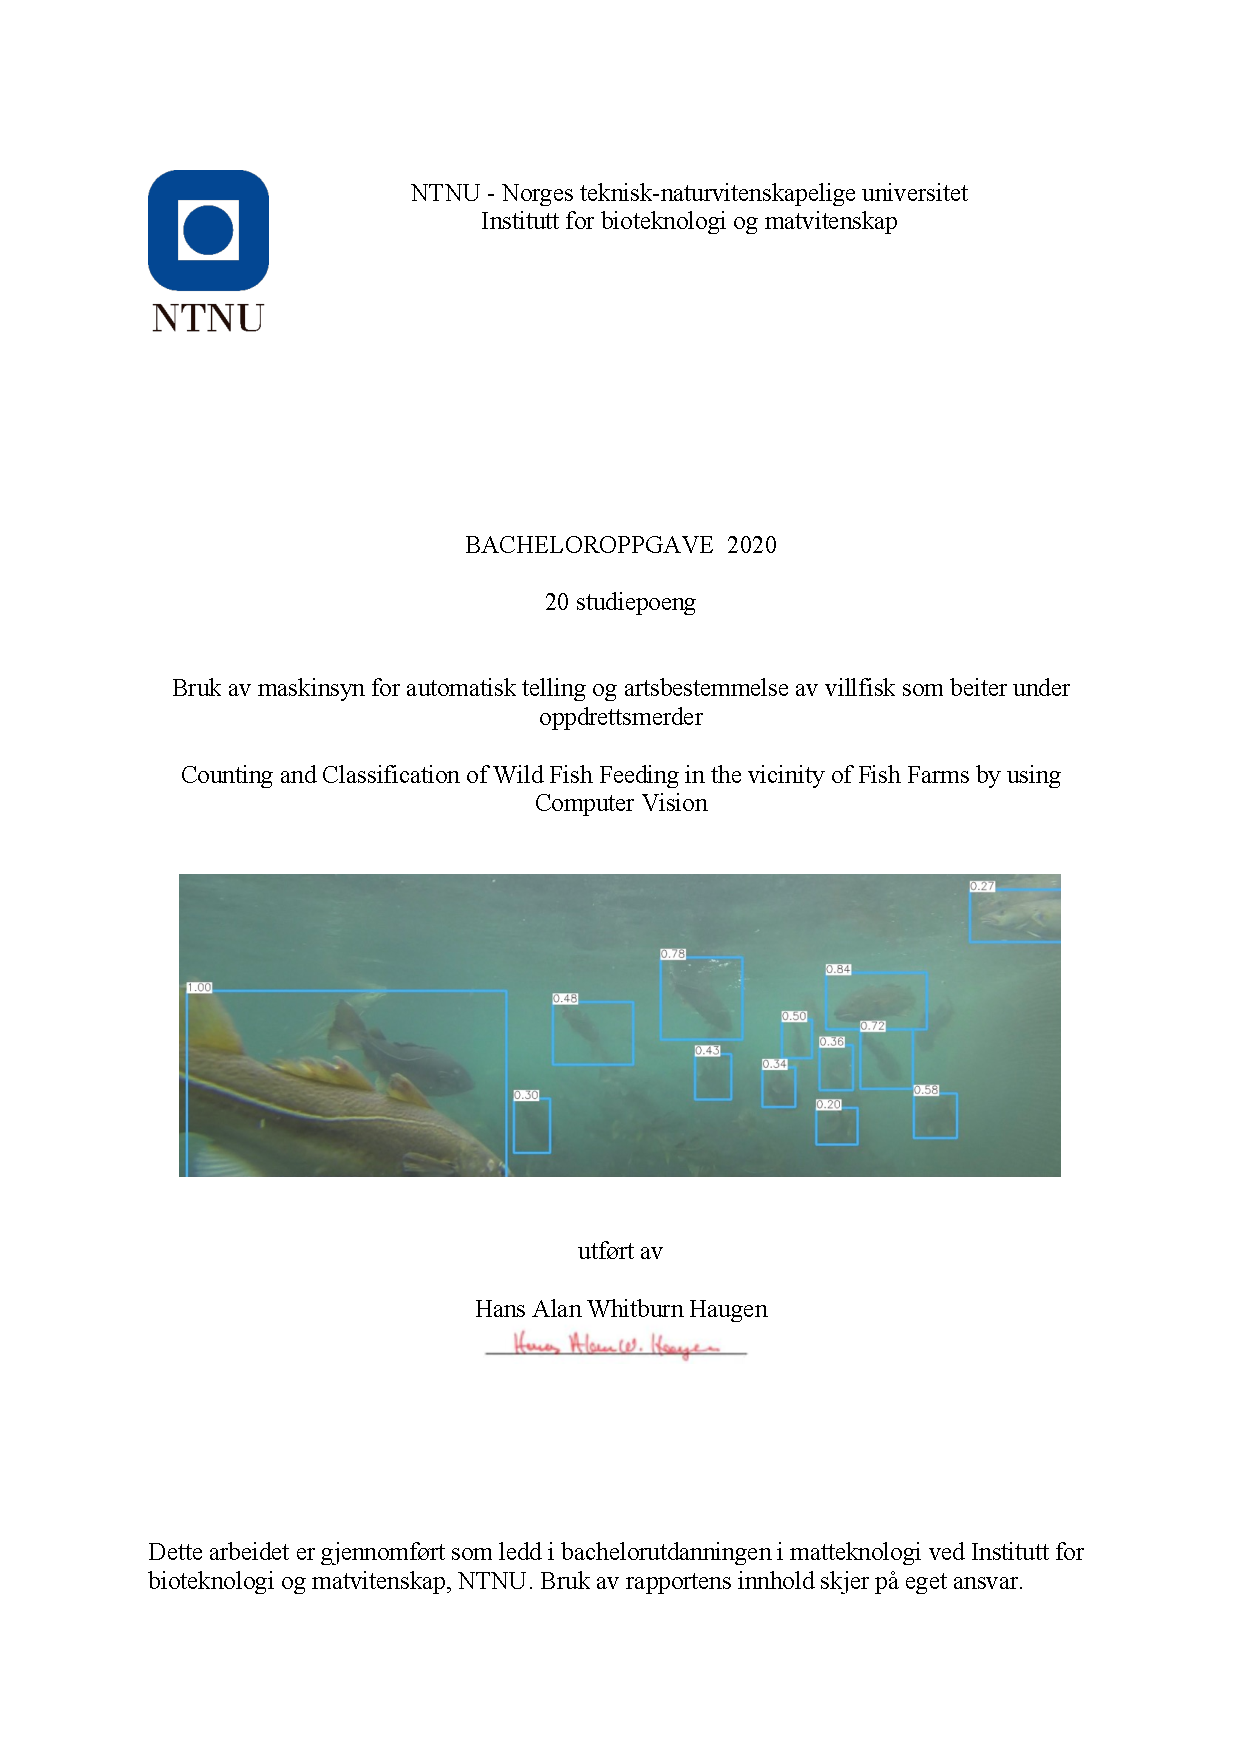
\includepdf[fitpaper=true, pages=-]{forsidemal.pdf}

\newpage
\section*{Sammendrag}

%Lengre oppgaver, som bachelor- og masteroppgaver, skal ha et sammendrag. Det er viktig at sammendraget er informativt, siden det skal kunne leses av lesere som ikke er eksperter på området.

%Sammendraget skal være kort, helst ikke over én A4-side, og skal gi et overblikk over hovedinnholdet. Du skal fortelle leseren:

%hva du har undersøkt

Fôrsprengt fisk har blitt vanlig i Lyngen kommune i Troms. ``Pellets-fisk” ble vanlig etter at de begynte med oppdrett i fjorden. Fisken er full av fôr og stinker. Den er unaturlig og tjukk.

``Pellets-fisk'' er villfisk som har spist oppdrettsfôr som inneholder medisin. Denne fisken blir omsatt. Et eksempel er når lakselusmiddelet emamectin ble gitt til oppdrettsfisk i tre uker i 2017 i denne fjorden i Lyngen. Oppdrettsfisken var i karantene i denne perioden, og blir ansett som giftig. I samme periode leverte fiskere villfisk fra denne fjorden til et mottak i Troms. Den var full av pellets. Det sto ut av munnen på både sei og torsk.

Det er et ønske å kartlegge omfanget av problemet, og fiskere vil ha svar på om pellets-fisken kan være farlig. Det er et ønske å kartlegge hvor mange villfisk som trekker til oppdrettsanlegg, og under hvilke forhold. Sjømatdivisjonen og Akvadivisjonen ved Nofima har en strategisk internsatsing å samle kunnskap om sameksistens mellom ulike marine næringer og interesser, deriblant hvordan man kan unngå konflikter mellom ulike interesser.

Dette prosjektet har gått ut på å lage programvare for Nofima som kan skape en oversikt over mengden fisk av typen torsk og sei som beiter rundt oppdrettsanlegg, og som viser fordelingen av fiskeartene til forskjellige tider på døgnet.

%hvordan du gjorde det

Maskinlæring er når datamaskiner lærer fra data. I 2012 vant AlexNet Stanford University sin årlige ImageNet bildeklassifiseringskonkurranse. Teamet til Alex anvendte deep learning og det har revolusjonert maskinsyn og kunstig intelligens. Flere modeller har blitt laget siden AlexNet, og bildeklassefisering, objektdeteksjon og segmentering har blitt mye mer nøyaktig nå som de anvender dype kunstige neurale nettverk. Facebook introduserte RetinaNet i 2017, og i 2018 kom YOLOv3. Det er disse teknologiene som har blitt anvendt til å lage en modell som kan kjenne igjen torsk og sei med ...(resultater) .

%hva du fant ut

Prosjektet viser at maskinsyn kan anvendes til å løse oppgaver innenfor akvakultur. Teknologien som presenteres i dette dokumentet kan anvendes til å finne omfanget av torsk og sei som beiter rundt oppdrettsanlegg, og kan muligens anvendes til å detektere rømninger fra merder samt utvikles videre til å detektere lakselus på fisk i merdene.

%Ved å lese sammendraget skal leserne kunne avgjøre om de er interessert i å lese resten av teksten.
\newpage
\section*{Forkortelser og faguttrykk}

\begin{description}

\item[Maskinsyn] Computer Vision has become ubiquitous in our society, with applications in search, image understanding, apps, mapping, medicine, drones, and self-driving cars. Core to many of these applications are visual recognition tasks such as image classification, localization and detection. Recent developments in neural network (aka “deep learning”) approaches have greatly advanced the performance of these state-of-the-art visual recognition systems. This course is a deep dive into details of the deep learning architectures with a focus on learning end-to-end models for these tasks, particularly image classification. During the 10-week course, students will learn to implement, train and debug their own neural networks and gain a detailed understanding of cutting-edge research in computer vision. The final assignment will involve training a multi-million parameter convolutional neural network and applying it on the largest image classification dataset (ImageNet). We will focus on teaching how to set up the problem of image recognition, the learning algorithms (e.g. backpropagation), practical engineering tricks for training and fine-tuning the networks and guide the students through hands-on assignments and a final course project. Much of the background and materials of this course will be drawn from the ImageNet Challenge.
\item{Backpropagation}
\item{ImageNet}
\item{COCO}
\item{Deep Learning}
\item[ML] Machine Learning
\item[CPU] Central Processing Unit
\item[GPU] Graphical Processing Unit
\item[YOLO] You Only Look Once
\item[FPS] Frames Per Second
\item[State-of-the-art] 
\item[Real-time] Sanntid
\item[mAP] 
\item[Nøyaktighet] 
\item[Presisjon] 
\item[Modell] 
\item[Algoritme]


\end{description}
\newpage
\section*{Takk}

Jeg ønsker å takke min veileder Eirin Bar. Oppgaven ble påbegynt 9. mars og foregikk frem til i dag, jeg hadde ikke gjennomført oppgaven uten veiledningen jeg fikk. Koronaviruspandemien av 2020 førte til at arbeidet i sin helhet ble gjort i Trondheim.

Jeg ønsker å takke Karsten Heia og spesielt Stein-Kato Lindberg fra Nofima. Det var KVASS-prosjektet\footnote{\url{https://nofima.no/prosjekt/kvass/}} til Nofima som gjorde at jeg kontaktet dem og spurte om jeg kunne gjøre bacheloroppgaven i samarbeid med dem. Det har vært en drøm å jobbe på en bacheloroppgave som handler om maskinsyn. Stein-Kato foreslo at jeg tok del i sameksistens prosjektet, og har bidratt med data, hyggelige tilbakemeldinger og råd.

I tillegg ønsker jeg også å takke Satya Mallick, Vikas Gupta, Anastasia Murzova, Anna Petrovicheva, Grigory Serebryakov, Pavel Semkin, Prakash Chandra, Sergei Belousov, Tatiana Khanova og Valeriia Koriukina for utmerkede kurs ved \url{courses.opencv.org}.

\begin{flushright} 

\includegraphics{figures/underskrift}\\ \ Trondheim \ \today
\end{flushright} 

%It is with great pride I hereby present my bachelor thesis. During this three month long process, I have gained a lot of knowledge of this research and it has been beneficial to my development in furthering my career and my studies in the future. I would like to express absolute gratitude to my beloved supervisor, Ms. Eirin Bar for her kind words, encouragement and persistent support in my understanding of this research. God bless her!

%I would like to express my appreciation to all Rock bands in the 80s to both iconic rock band for inspiring me to do this thesis. Lastly, this research would not have been completed without the support and motivation from my beloved family, friends, colleagues, lecturers, classmates who has been with me through thick and thin during this marvelous adventure in completing our bachelor degree. Above all, to the Great Almighty, for his countless blessings.
\newpage

\tableofcontents
\clearpage
\pagenumbering{arabic}
\setcounter{page}{1}

\section{Innledning}

%I innledningen skal du plassere deg i fagfeltet og vise at du har kjennskap til tidligere forskning. Innledningen skal gjøre rede for hva vi vet og hva vi ikke vet om feltet.

%Dette gjør du ved å presentere:

%et problem eller et fenomen du skal studere

\begin{figure}[h!]
\begin{center} 
\includegraphics[scale=0.05]{../data/train/atlantic_cod/fish_2690}
\includegraphics[scale=0.05]{../data/train/atlantic_cod/fish_6040}
\includegraphics[scale=0.05]{../data/train/atlantic_cod/fish_8540}
\includegraphics[scale=0.05]{../data/train/atlantic_cod/fish_10440}
\includegraphics[scale=0.05]{../data/train/atlantic_cod/fish_4940}
\includegraphics[scale=0.05]{../data/train/atlantic_cod/fish_5740}
\caption{\small \sl Figuren viser eksempelbilder fra en video av en lagringsmerd med torsk. Disse bildene er en del av datasettet anvendt for deteksjon av torsk og sei. \label{fig:data}} 
\end{center} 
\end{figure} 

Her presenteres automatisk fiskedeteksjon av torsk og sei i bilder tatt med undervannskameraer. Modellen er trent opp på fisk fra merder brukt til fiskeoppdrett og lagring. Se figur \ref{fig:data}.

Dette arbeidet er viktig for å forstå omfanget av torsk og sei som trekker til oppdrettsanlegg og spiser oppdrettsfôr fra under merdene. Forskere, samt fiskere og oppdrettsnæringen, ønsker å samle informasjon om villfisk som spiser oppdrettsfôr, fôret kan til forskjellige tider inneholde medisinrester.

Manuell analyse av data fra undervannskameraer er tidskrevende, dessuten kan det kreve ekspertkunnskap om forskjellige fiskearter. Dette gjør det veldig vanskelig å gjennomføre et større datainnsamlingsprosjekt. Til tross for vanskelighetene så er slike analyser viktige. Kunnskap om de marine økosystemene, og effekten oppdrettsnæringen har på mattrygghet og kvalitet av villfisk, berører fiskere og befolkningen som spiser norsk fisk. Dessuten kan teknologien brukes for å unngå overfôring, noe som bidrar til at oppdrettsbedrifter sparer penger. Derfor er verktøy som gjør automatisk videoanalyse nødvendig, og bør utvikles for å støtte forskere i arbeidet deres.

Dette prosjektet er gjort i samarbeid med Nofima som en del av Sameksistensprosjektet \cite{Robertsen 2020}. Dataprogrammet som har blitt utviklet for denne oppgaven kan ta imot undervannsvideo med høy oppløsning og telle antall norsk torsk, $Gadus$ $morhua$, og sei, $Pollachius$ $virens$, fortløpende. Se figur \ref{fig:inference}.

\begin{figure}
\begin{center} 
%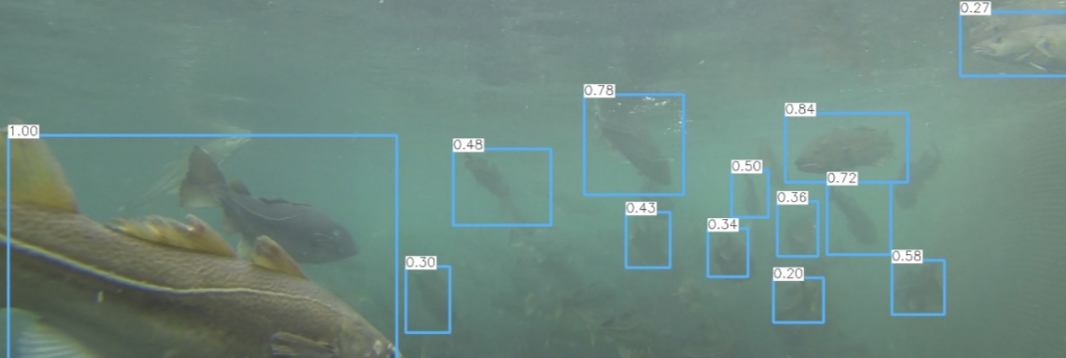
\includegraphics[scale=0.6]{figures/cover}
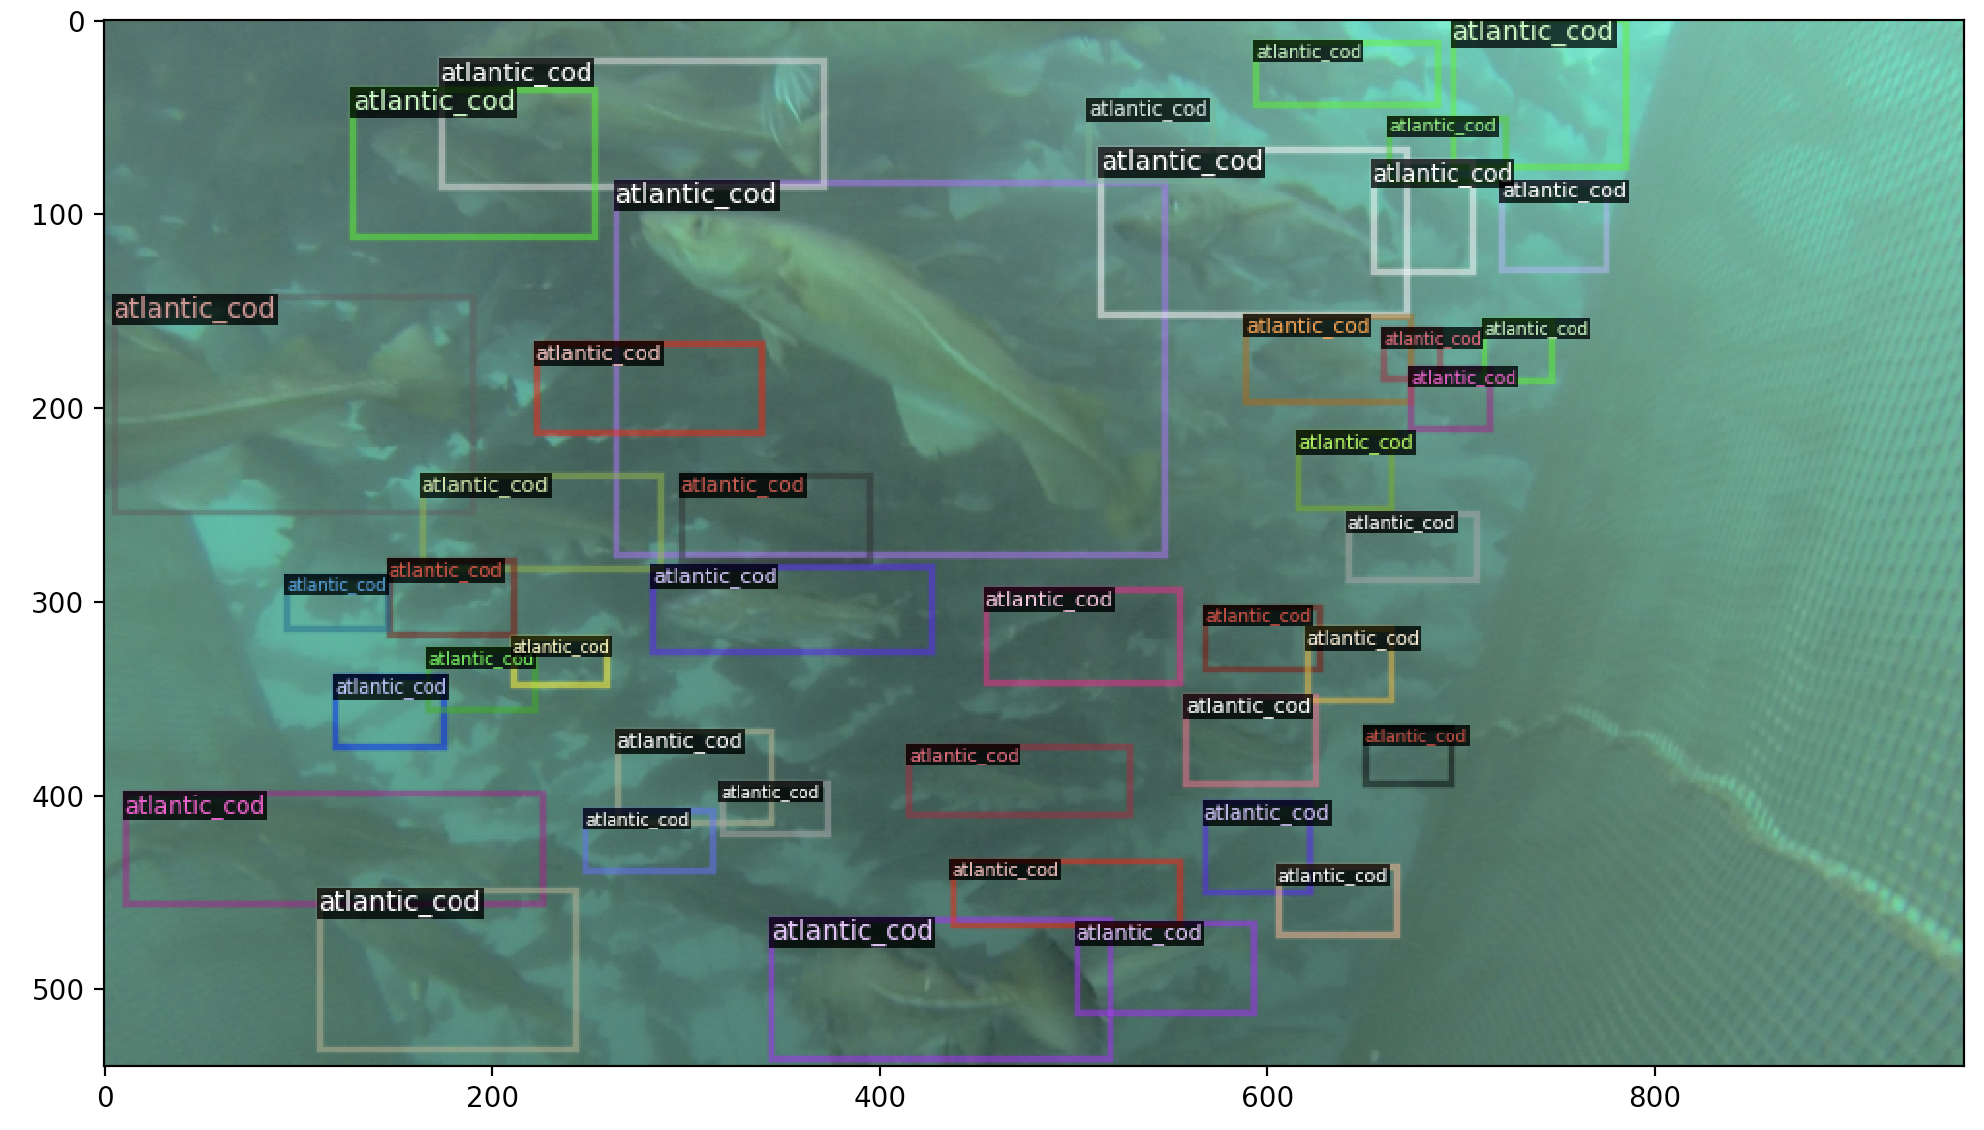
\includegraphics[scale=0.35]{figures/retinanet_cod_2}
\caption{\small \sl Figuren viser inferens med en RetinaNet model. Råbilde er fra en video av en lagringsmerd med torsk. Modellen ble trent som en del av dette bachelorprosjektet. \label{fig:inference}} 
\end{center} 
\end{figure} 

%bakgrunnen for valg av tema
%problemstillingen eller hypotesene du skal undersøke
%På slutten av introduksjonen kan du også si noe om hvordan du har tenkt å strukturere resten av oppgaven, som en kort leserguide.

%Et tips er å begynne å skrive på innledningen tidlig, slik at den kan gi retning for det videre arbeidet ditt. Så går du heller over innledningen igjen på slutten for å skrive den helt ferdig. Da får du en innledning som har god sammenheng med resten av teksten.

\subsection{Bakgrunn}

\begin{figure} 
\begin{center} 
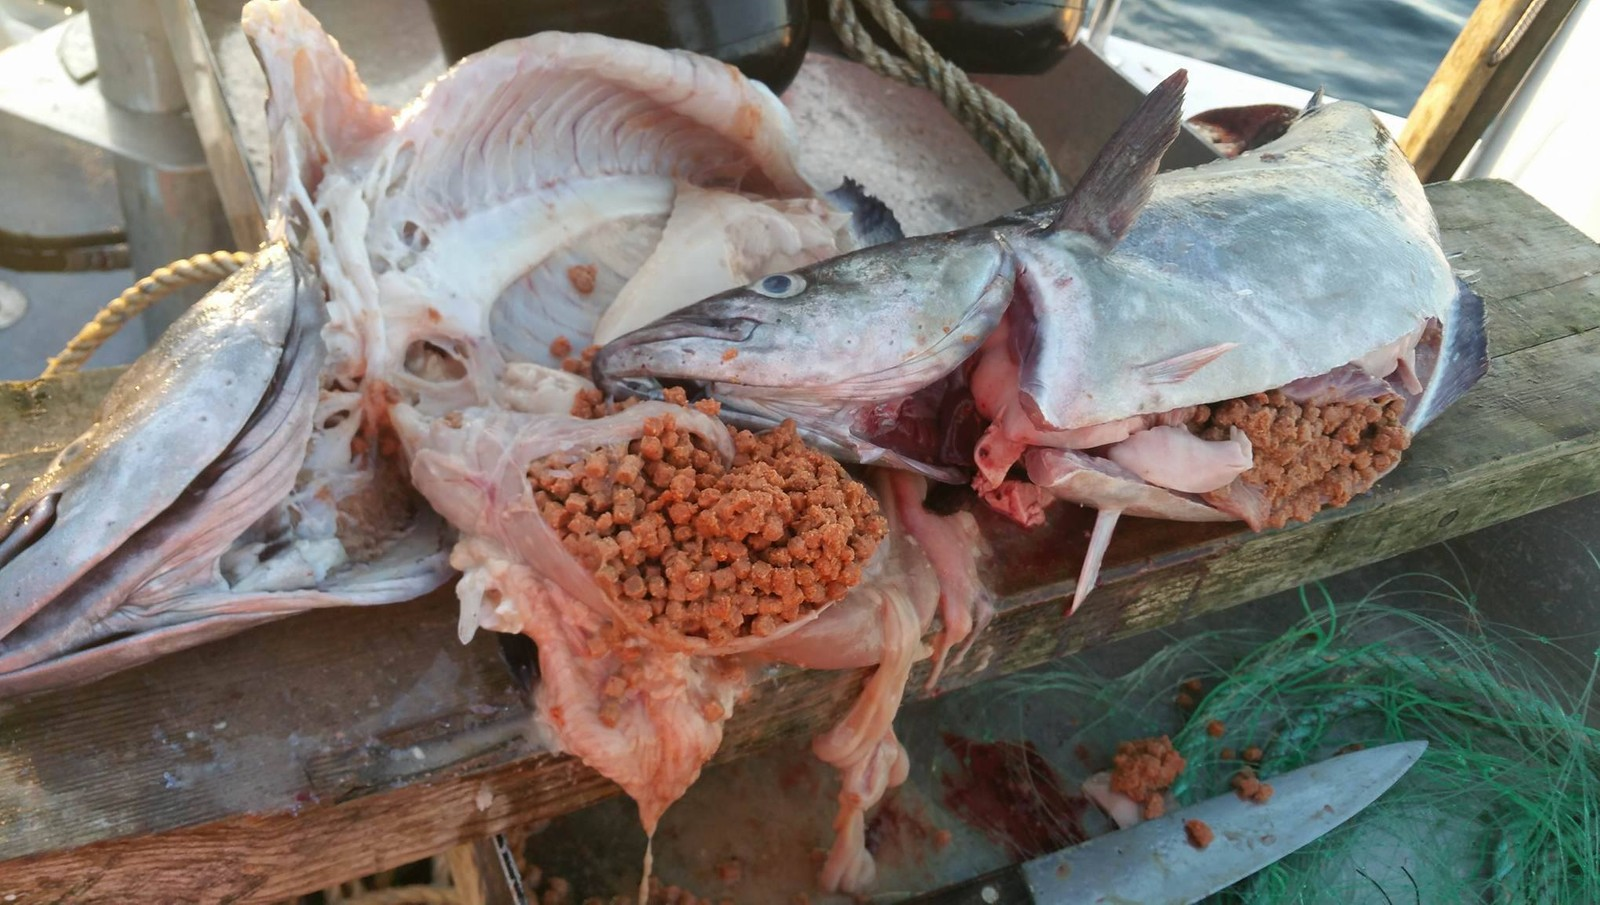
\includegraphics[scale=0.2]{figures/oppdrettfor}
\caption{\small \sl Figuren viser et eksempel av ``pellets-fisken''. Det lukter ekkelt og det er forferdelig å sløye en fôrsprengt fisk, ifølge flere fiskere som har vært i kontakt med NRK \cite{Trana m.fl. 2019}. Seien har vært under merdene, da blir den full av pellets. Fôrsprengt fisk er unaturlig, hode blir for liten og kroppen for stor. Dette har pågått i mange år. Likevel blir fisken omsatt, fiskere får levert slik fisk til enkelte fiskebruk. \cite{Angell og Ekanger 2017} \label{fig:oppdrettfor}} 
\end{center} 
\end{figure} 

\begin{figure}
\begin{center} 
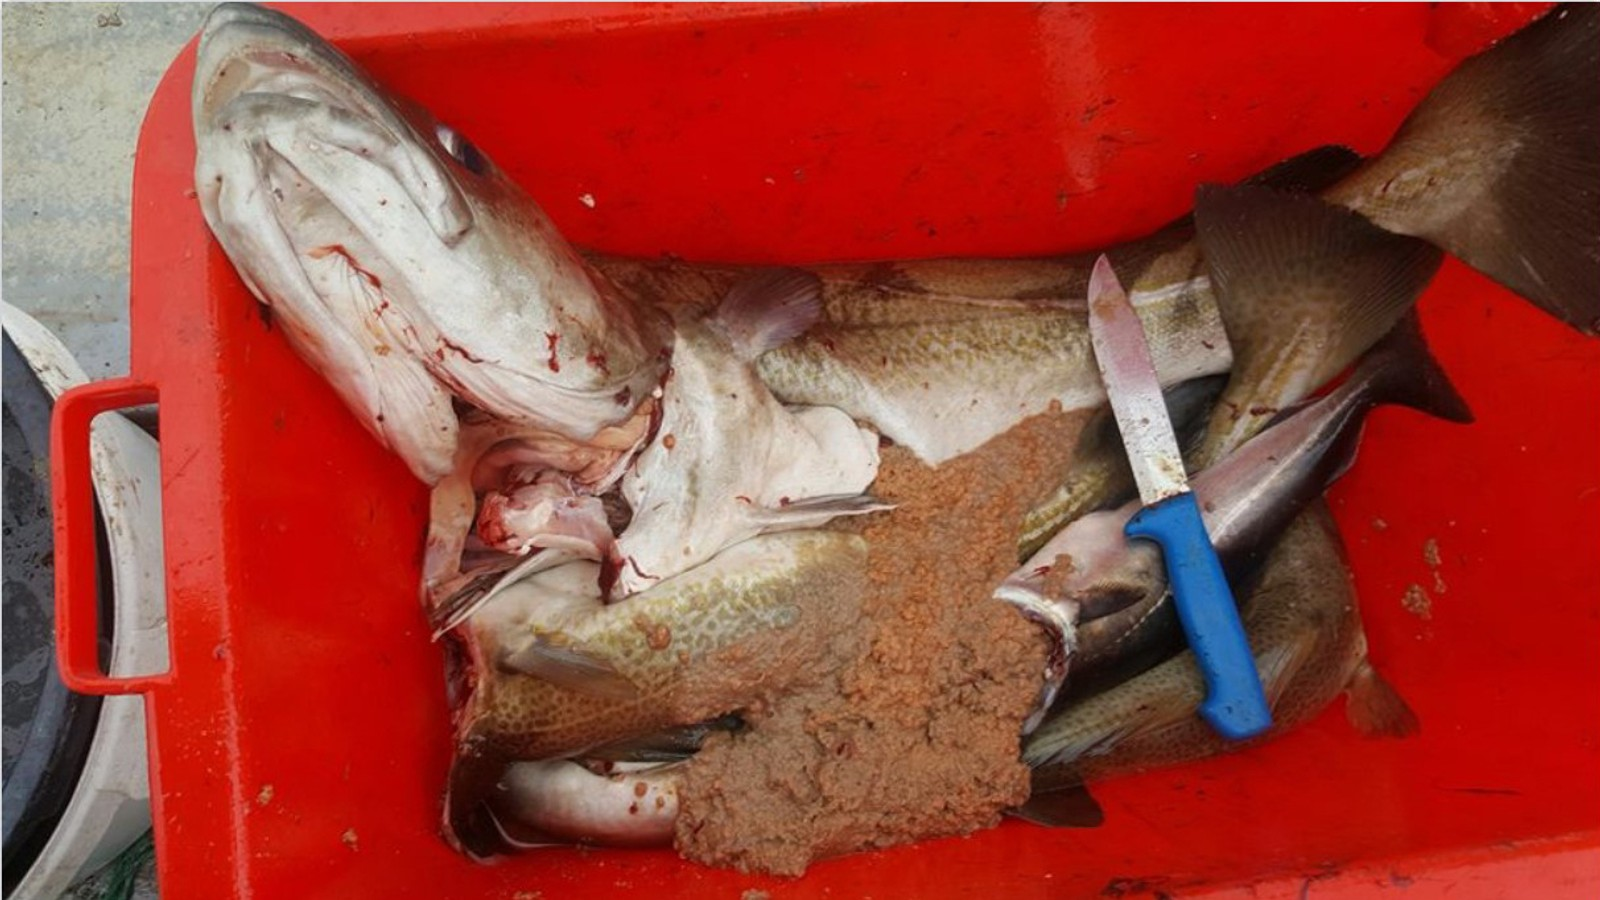
\includegraphics[scale=0.2]{figures/forsprengt}
\caption{\small \sl Figuren viser et eksempel av fôrsprengt fisk. Det lukter ekkelt og det er forferdelig å sløye en fôrsprengt fisk, ifølge flere fiskere som har vært i kontakt med NRK. Foto: Arnold Jensen. \cite{Trana m.fl. 2019} \label{fig:forsprengt}} 
\end{center} 
\end{figure} 

Kystfiskere hevder villfisken får i seg så mye laksefôr at fiskeplassene blir ødelagt. Fisker Tor Inge Larsen i Brønnøysund sa til NRK i 2018 at han fortviler over det han mener er dårligere kvalitet hos fisken han fanger. Han sa han kan knapt huske sist han fikk en sei om bord i båten uten at den hadde pellets fra lakseoppdrett i magen. Han hevder fiskerne har blitt frastjålet fiskeområder på høylys dag, og mener fiskefeltene nært Brønnøysund på Sør-Helgeland i Nordland har fått betydelig lavere kvalitet på grunn av oppdrettsanleggene. \cite{Olsen m.fl. 2018}

%Hvis jeg kan foreslå en mulig forbedring så kan første del av avsnitt 1.1 skrives litt mer sammenfattet, for eksempel med et par avsnitt om hvilke grupper som er negative til «pelletsfisk», og et par avsnitt om hvem som er positive eller likegyldig til det. Her kan du også vise til en spørreundersøkelse som er gjort på sameksistensprosjektet. Den er ikke publisert enda, men forskerne har skrevet en bloggartikkel om den https://blogg.forskning.no/fra-fjord-til-bord/hvem-bryr-seg-om-pelletssei/1648846.

Men ikke alle er negative til ``pelletsfisk''. Nofima gjorde en undersøkelse i 2020 som viser hvilke grupper som er negative, positive eller likegyldig til fisken. Nofima forskerne Anette Hustad og Ragnhild Svalheim oppdaget at de fleste er nøytrale til påstander om at pelletssei smaker eller lukter annerledes enn annen sei. De konstaterer at matopplevelser er påvirket av følelser. ``Å synes noe er uappetittlig, er en personlig, subjektiv følelse og den er nok ganske uavhengig av hva den objektive forskningen sier''. \cite{Hustad og Svalheim 2020}

Andre forskere har også vært uenige om hvorvidt pellets fra lakseoppdrett påvirker kvaliteten av villfisk som spiser den. Det er forsket relativt lite på hvordan oppdrett påvirker villfisk, men seniorrådgiver Bjørn-Steinar Sæther fra Nofima ga ut en artikkel i 2017 der han viste at seien som hadde spist oppdrettsfôr får en litt bløtere og noe mer spaltet muskel enn annen sei. Ellers var kvaliteten fortsatt stort sett innenfor kategorien god kvalitet. \cite{Saether 2017}

%Det kan også være greit å legge mer vekt på at oppdrettsnæringen er interessert i å kartlegge hvor mye fôr som spises av villfisk. Det er viktig for dem å ha kontroll på fôrmengden som går til spille siden det er en stor kostnad som har økt mye de siste årene (se f. eks. https://www.fhf.no/nyheter/nyhetsarkiv/kostnadene-for-norsk-lakseoppdrett-fortsetter-aa-oeke-ogsaa-i-2019/). Man kan derfor si at dette prosjektet vil være positivt for både fiskere og oppdrettere.

Oppdrettsnæringen er også interessert i å kartlegge hvor mye fôr som spises av villfisk. I 2019 avsluttet FHF, Fiskeri- og havbruksnæringens forskningsfinansiering, et prosjekt ledet av Audun Iversen fra Nofima der de så på kostnadsutvikling og forståelse av drivkrefter i norsk lakseoppdrett. For oppdrettsnæringen er å ha kontroll på fôrmengde som går til spille viktig, fôrpellets er en stor kostnad som har økt mye de siste årene. De ønsker ikke å fôre oppdrettsfisken mer enn nødvendig, om problemet løses så vil det bli mindre oppdrettsfôr til villfisken. \cite{Baevre-Jensen 2019}

%Johnny Eliassen som er bosatt på Reinøya i Troms, Karlsøy kommune, fortalte til NRK at han hadde tidligere engasjert seg i saken for å hindre at kystområdet ble lokasjon for oppdrettsanlegg. Det ble allikevel åpnet et oppdrettsanlegg mai 2017 i fjorden på Reinøya, og det hevder de lokale fiskerne at de har merket. De har fisket ``pelletstorsk'',  torsk med magen full av pellets, selv over en kilometer unna anlegget. Oppdrettere reklamerer oppdrettsfisk som den absolutte beste fisken. Eliassen kunne ikke tenke seg er at det virkelig er tilfelle, for lukten og konsistensen på fisken gjør den uspiselig i hans øyne. \cite{Jakobsen 2017}

Kommunikasjonsdirektør Are Kvistad i Sjømat Norge er litt overrasket over utspillet fra fiskeren på Helgeland. Han mener laksepellets ikke utgjør noen fare for villfisk. ``Det er et fiskefôr som blir sjekket av myndighetene, og er et trygt og næringsrikt fôr som også er trygt for villfisk'', sa Kvistad til NRK i 2018. Kvistad mente det også er i oppdretternes interesse, både økonomisk og utslippsmessig, å redusere fôringen av oppdrettslaksen slik at den kun får den maten den trenger. \cite{Olsen m.fl. 2018}

%Vinteren 2018 rømte 52 000 laks fra Marine Harvests oppdrettsanlegg i Nærøy kommune i Trøndelag. Ifølge Namdalsavisa inneholdt laksen medisiner mot innvollsorm. Mattilsynet gikk ut og sa at det var trygt å spise fisken, men at den ikke kunne omsettes videre. \cite{nrk 2018}

%Den rømte laksen hadde blitt gitt medisinfôr med praziquantel og skulle være i karantene i 14 dager. For fiskere, slik som Arnold Jensen, er denne informasjonen skremmende. Jensen er medlem av Naturvernforbundets fiske- og oppdrettsutvalg. Han ønsker at mattryggheten til villfisk som beiter ved oppdrettsanleggene skal kontrolleres. Se figur \ref{fig:oppdrettfor} og \ref{fig:forsprengt}. \cite{Christensen 2019}

I 2019 kom ``pellets-fisken'' i medienes søkelys igjen, denne gangen var det fiskere i Lyngen kommune i Troms som slo alarm. Villfisk som hadde spist oppdrettsfôr som inneholdt medisin ble omsatt av fiskere i fjorden. Oppdrettsfisken var i karantene i denne perioden. Fiskerne ønsket svar på om villfisken kan være farlig for forbrukere. \cite{Trana m.fl. 2019}

\begin{figure} 
\begin{center} 
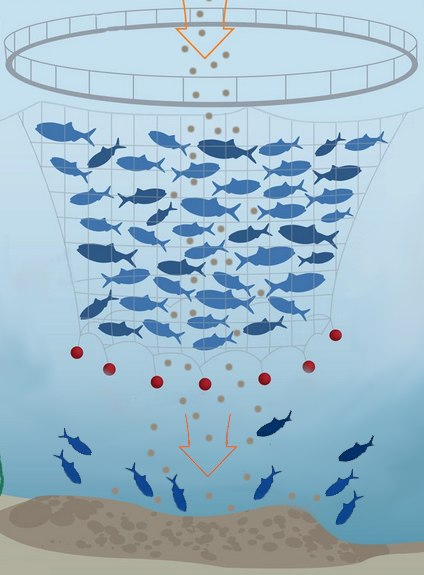
\includegraphics[scale=0.7]{figures/merder-fisk}
\caption{\small \sl Figuren viser et oppdrettsanlegg \cite{Spruill 2011 s. 12}. Fôret oppdrettsfisken mates med spises også av villfisk. Oppdrettsbransjen er i konflikt med fiskere som mener oppdrettsnæringen ødelegger fiskeplasser i fjordene med anlegg og reduserer kvaliteten til villfisk som spiser fôrpellets under merdene. \cite{Olsen m.fl. 2018} \label{fig:anlegg}} 
\end{center} 
\end{figure} 

%\begin{figure} 
%\begin{center} 
%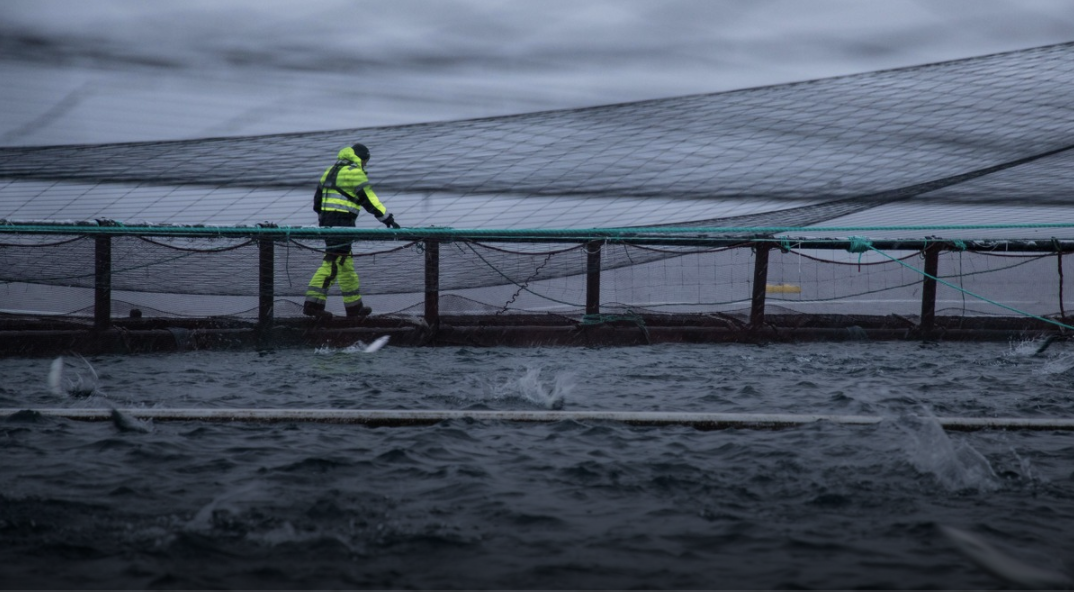
\includegraphics[scale=0.7]{figures/oppdrett}
%\caption{\small \sl Figuren viser et oppdrettsanlegg. Fôret oppdrettsfisken mates med spises også av villfisk. Oppdrettsbransjen er i konflikt med fiskere som mener oppdrettsnæringen ødelegger fiskeplasser i fjordene med anlegg og reduserer kvaliteten til villfisk som spiser fôrpellets under merdene. \cite{Olsen m.fl. 2018} \label{fig:anlegg}} 
%\end{center} 
%\end{figure} 

Sjømatdivisjonen og Akvadivisjonen ved Nofima har en strategisk internsatsing som går ut på å samle kunnskap om sameksistens mellom ulike marine næringer og interesser, deriblant om hvordan man kan unngå konflikter mellom ulike interesser. Se figur \ref{fig:anlegg}. \cite{Robertsen 2020}

En av problemstillingene er sameksistens mellom fiskeri- og oppdrettsnæringene, og hvordan oppdrettsanlegg påvirker de nærliggende fiskeplassene. I den forbindelse er det interessant å kartlegge omfanget av hvitfisk som beiter på fôr fra oppdrettsanlegg. Dette er en problemstilling som har vært i fokus hos media etter at flere fiskere har fanget fôrsprengt torsk og sei i fjorder hvor det finnes oppdrettsanlegg. Det hevdes at denne fisken er av betydelig dårligere kvalitet og den kan ha fått i seg medisiner gjennom fôret som gjør at den kan være farlig å spise. \cite{Olsen 2019}

Det behøves kunnskap om hvor mange villfisk som trekker til oppdrettsanlegg, og under hvilke forhold, slik at man kan komme nærmere en løsning som kan dempe konflikten mellom disse to næringene. 

Målet med dette prosjektet var å utvikle et system som kan telle antall villfisk av ulike arter basert på en videostrøm fra et undervannskamera. Det er ønskelig å kunne vise resultatet som en fordeling av observasjoner over tid for hver art. 

\subsection{Kunstig intelligens}

\begin{figure} 
\begin{center} 
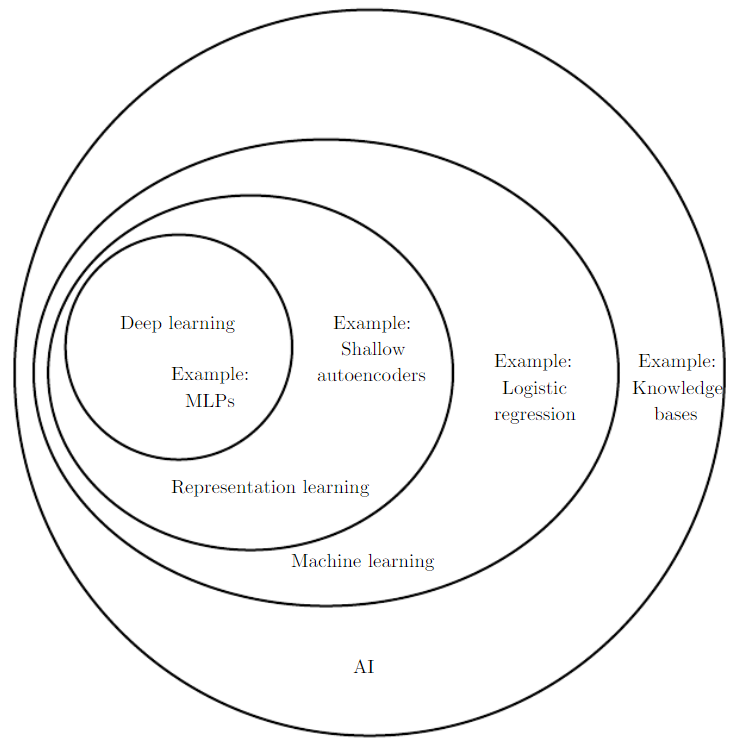
\includegraphics[scale=0.7]{figures/ai}
\caption{\small \sl Figuren viser et Venn diagram som viser at deep learning er en form for representativ læring, og det er igjen en form for maskinlæring. Maskinlæring er anvendt i mange, men ikke alle, de forskjellige metodene innenfor kunstig intelligens. Hver del av Venn diagrammet gir et eksempel av anvendelsen til teknologien. \cite{Goodfellow m.fl. 2016 s. 9} \label{fig:ai}} 
\end{center} 
\end{figure} 

Tilbake på 1840-tallet, da programmering av datamaskiner ble oppfunnet, så spurte matematikere av den tiden seg selv om slike maskiner kunne bli intelligente, selv over hundre år før en datamaskin faktisk hadde blitt bygget (Lovelace 1842). I dag så har kunstig intelligens (KI) blitt et stort forskningsfelt med mange praktiske anvendelser og aktive forskningsprosjekter. Intelligent programvare automatiserer trivielt og repetitivt arbeid, forstår tale og kjenner igjen objekter i bilder, kan diagnosere pasienter innenfor medisin og hjelper forskere med grunnforskning. KI kan finne mønstre i store datamengder som det er vanskelig for mennesker å få øye på. \cite{Goodfellow m.fl. 2016 s. 1}

Dette prosjektet beskriver maskiner som kan gi en tidsoversikt over torsk og sei fra en videostrøm. Den lærer konseptene en torsk eller sei består av, den lærer fra data. Maskinlæring, å la en maskin lære fra data, er kun en av metodene innenfor kunstig intelligens. Se figur \ref{fig:ai}. Kunstig intelligens har vært igjennom to ``vintre'', men de siste åtte årene har vært en ny gullalder for kunstig intelligens etter introduksjonen av AlexNet i 2012. \cite{Canziani m.fl. 2017 s. 1}

I begynnelsen så løste kunstig intelligens problemer, med fremragende hastighet, som var intellektuelt vanskelige for mennesker å løse, men relativt trivielle for datamaskiner. Problemene kunne beskrives formelt, med matematiske regler. Utfordringen med kunstig intelligens viste seg å være å løse problemer som var enkle for mennesker å utføre, men vanskelige for mennesker å beskrive formelt. Dette er problemer som vi løser intuitivt, som føles automatiske ut, slik som å forstå ordene til andre mennesker, ansiktene deres, og å kjenne igjen det en har sett tidligere i bilder. \cite{Goodfellow m.fl. 2016 s. 1}

Denne oppgaven handler om å finne løsninger på intuitive problemer. Løsningen er å la datamaskiner lære fra erfaringer og forstå verden ved å forstå konsepter, som kan igjen bli forstått med enda enklere konsepter. Denne samlingen av kunnskap fra erfaring som datamaskinene gjør seg selv, uten at et menneske formelt beskriver kunnskapen til maskinen, kan beskrives med en graf. Se figur \ref{fig:deep}. Ettersom denne grafen kan bestå av mange lag, den er dyp, så kalles denne formen for maskinlæring ``deep learning'' \cite{Goodfellow m.fl. 2016 s. 1}.

%"Deep Learning" is a general term that usually refers to the use of neural networks with multiple layers that synthesize the way the human brain learns and makes decisions. A convolutional neural network is a kind of neural network that extracts features from matrices of numeric values (often images) by convolving multiple filters over the matrix values to apply weights and identify patterns, such as edges, corners, and so on in an image. The numeric representations of these patterns are then passed to a fully-connected neural network layer to map the features to specific classes. https://notebooks.azure.com/graememalcolmoutlook/projects/mlprimers/html/05a%20-%20Image%20Classification%20with%20a%20CNN%20(PyTorch).ipynb

\begin{figure} 
\begin{center} 
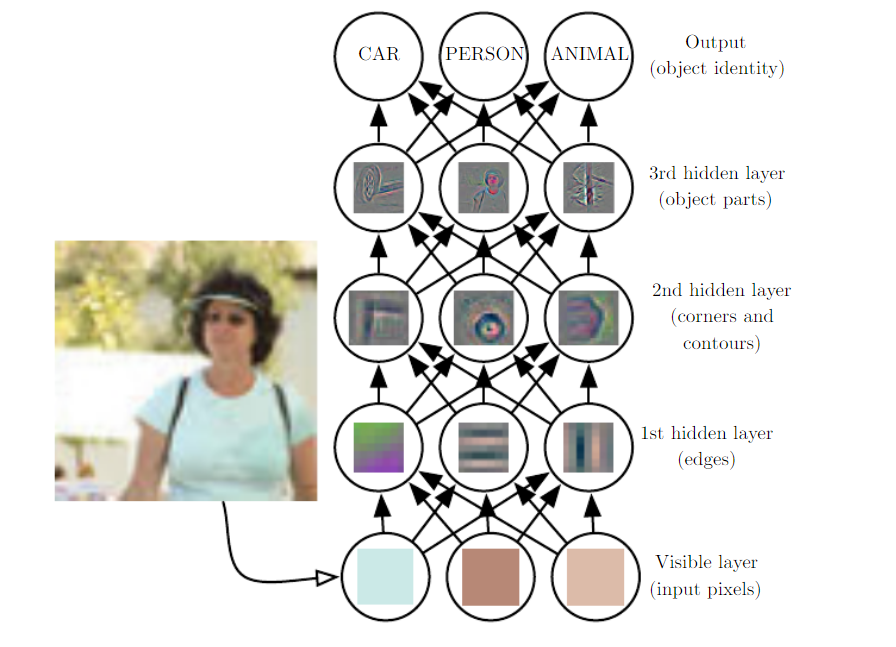
\includegraphics[scale=0.65]{figures/deep}
\caption{\small \sl Figuren viser en deep learning modell. Det er vanskelig for en datamaskin å forstå hva en matrise av sensorisk rådata er, slik som dette bildet representert som en samling pikselverdier, en matrise. Å lage en funksjon som tar inn piksler og gir ut en objektidentitet er svært komplisert. Å utlede en slik funksjon virker nærmest umulig om en takler problemet direkte. Deep learning løser vanskelighetene ved dele opp den kompliserte funksjonenen til en samling sammenkoblede funksjoner. Disse funksjonene kalles ofte for kunstige nevroner, kerneler, perceptrons eller filtere. Utmatningene fra kernelene i ett lag blir innmatningene til neste lag i modellen. Innmatningen til modellen, slik som et bilde, kalles for det synlige laget, ettersom den består av informasjon som vi mennesker kan forstå. Dette laget er etterfulgt av en serie med skjulte lag, ``hidden layers'', hvert lag henter ut mer og mer abstrakte konsepter, ``features'', fra bildet. Disse lagene kalles for ``hidden'' ettersom verdiene i disse lagene ikke finnes i innmatningen til nettverket; modellen må selv bestemme hvilke konsepter som er nyttige for å beskrive sammenhengen i det synlige laget. Hvert lag danner forskjellig innsikt. Det første laget kan for eksempel lett gjenkjenne kantene i et bilde ved å sammenligne kontraster i bildet. Denne informasjonen sendes til det neste laget, et lag som finner kanter. Gitt det andre skjulte lagets beskrivelse av bildet, et bilde beskrevet med kanter, så kan objektdeteksjon bli mulig ved å sammenligne en samling kanter, konturer, med deler av kjente objekter. \cite{Goodfellow m.fl. 2016 s. 6} \label{fig:deep}} 
\end{center} 
\end{figure} 

%The difficulties faced by systems relying on hard-coded knowledge suggestthat AI systems need the ability to acquire their own knowledge, by extracting2
%CHAPTER 1. INTRODUCTIONpatterns from raw data. This capability is known asmachine learning. Theintroduction of machine learning enabled computers to tackle problems involvingknowledge of the real world and make decisions that appear subjective. A simplemachine learning algorithm calledlogistic regressioncan determine whether torecommend cesarean delivery (Mor-Yosef et al., 1990). A simple machine learningalgorithm called naive Bayes can separate legitimate e-mail from spam e-mail \cite{Goodfellow m.fl. 2020 s. 3}

%The performance of these simple machine learning algorithms depends heavilyon therepresentationof the data they are given. For example, when logisticregression is used to recommend cesarean delivery, the AI system does not examinethe patient directly. Instead, the doctor tells the system several pieces of relevantinformation, such as the presence or absence of a uterine scar. Each piece ofinformation included in the representation of the patient is known as afeature.Logistic regression learns how each of these features of the patient correlates withvarious outcomes. However, it cannot influence how features are defined in anyway. If logistic regression were given an MRI scan of the patient, rather thanthe doctor’s formalized report, it would not be able to make useful predictions.Individual pixels in an MRI scan have negligible correlation with any complicationsthat might occur during delivery. \cite{Goodfellow m.fl. 2020 s. 3}

%This dependence on representations is a general phenomenon that appearsthroughout computer science and even daily life. In computer science, operationssuch as searching a collection of data can proceed exponentially faster if the collec-tion is structured and indexed intelligently. People can easily perform arithmeticon Arabic numerals but find arithmetic on Roman numerals much more timeconsuming. It is not surprising that the choice of representation has an enormouseffect on the performance of machine learning algorithms. For a simple visualexample, see figure 1.1.

%Many artificial intelligence tasks can be solved by designing the right set offeatures to extract for that task, then providing these features to a simple machinelearning algorithm. For example, a useful feature for speaker identification fromsound is an estimate of the size of the speaker’s vocal tract. This feature gives astrong clue as to whether the speaker is a man, woman, or child.

%For many tasks, however, it is difficult to know what features should beextracted. For example, suppose that we would like to write a program to detectcars in photographs. We know that cars have wheels, so we might like to use thepresence of a wheel as a feature. Unfortunately, it is difficult to describe exactlywhat a wheel looks like in terms of pixel values. A wheel has a simple geometricshape, but its image may be complicated by shadows falling on the wheel, the sunglaring off the metal parts of the wheel, the fender of the car or an object in the foreground obscuring part of the wheel, and so on.

%One solution to this problem is to use machine learning to discover not onlythe mapping from representation to output but also the representation itself.This approach is known asrepresentation learning. Learned representationsoften result in much better performance than can be obtained with hand-designedrepresentations. They also enable AI systems to rapidly adapt to new tasks, withminimal human intervention. A representation learning algorithm can discover agood set of features for a simple task in minutes, or for a complex task in hours tomonths. Manually designing features for a complex task requires a great deal ofhuman time and effort; it can take decades for an entire community of researchers.

%The quintessential example of a representation learning algorithm is theau-toencoder. An autoencoder is the combination of anencoderfunction, whichconverts the input data into a different representation, and adecoderfunction,which converts the new representation back into the original format. Autoencodersare trained to preserve as much information as possible when an input is runthrough the encoder and then the decoder, but they are also trained to make thenew representation have various nice properties. Different kinds of autoencodersaim to achieve different kinds of properties.

%A major source of difficulty in many real-world artificial intelligence applicationsis that many of the factors of variation influence every single piece of data we areable to observe. The individual pixels in an image of a red car might be very closeto black at night. The shape of the car’s silhouette depends on the viewing angle.Most applications require us to disentangle the factors of variation and discard theones that we do not care about.

%Deep learningsolves this central problem in representation learning by intro-ducing representations that are expressed in terms of other, simpler representations.Deep learning enables the computer to build complex concepts out of simpler con-cepts. Figure 1.2 shows how a deep learning system can represent the concept ofan image of a person by combining simpler concepts, such as corners and contours,which are in turn defined in terms of edges.

%The quintessential example of a deep learning model is the feedforward deepnetwork, ormultilayer perceptron(MLP). A multilayer perceptron is just amathematical function mapping some set of input values to output values. Thefunction is formed by composing many simpler functions. We can think of eachapplication of a different mathematical function as providing a new representationof the input.

%Programvaren implementeres i C++ ved hjelp av OpenCV-biblioteket. Det kan også være aktuelt å lage et grafisk grensesnitt hvor tellingene fra hver art kan vises i sanntid, men dette er avhengig av om prosjektets omfang tillater det. \cite{opencv.org 2020}

%\subsection{Maskinsyn}

%\begin{figure} 
%\begin{center} 
%
\includegraphics[scale=0.7]{figures/digits}
%\caption{\small \sl Figuren viser tallene 504192. \cite{Nielsen 2019} \label{fig:digits}} 
%\end{center} 
%\end{figure} 

%Menneskets evne til å se er en av de mest fasinerende mirakelene i naturen. Folk flest kan uten anstrengelse gjenkjenne tallene 504192 i figur \ref{fig:digits}. At dette er lett er et under, og ikke minst misledende. In each hemisphere of our brain, humans have a primary visual cortex, also known as V1, containing 140 million neurons, with tens of billions of connections between them. And yet human vision involves not just V1, but an entire series of visual cortices - V2, V3, V4, and V5 - doing progressively more complex image processing. We carry in our heads a supercomputer, tuned by evolution over hundreds of millions of years, and superbly adapted to understand the visual world. Recognizing handwritten digits isn't easy. Rather, we humans are stupendously, astoundingly good at making sense of what our eyes show us. But nearly all that work is done unconsciously. And so we don't usually appreciate how tough a problem our visual systems solve.

%The difficulty of visual pattern recognition becomes apparent if you attempt to write a computer program to recognize digits like those above. What seems easy when we do it ourselves suddenly becomes extremely difficult. Simple intuitions about how we recognize shapes - "a 9 has a loop at the top, and a vertical stroke in the bottom right" - turn out to be not so simple to express algorithmically. When you try to make such rules precise, you quickly get lost in a morass of exceptions and caveats and special cases. It seems hopeless.

%Neural networks approach the problem in a different way. The idea is to take a large number of handwritten digits, known as training examples

\subsection{Tidligere arbeid}

Noen forskere har allerede rukket å anvende ``deep learning'' til å klassifisere fisk fra undervannsvideo. I 2016 presenterte CVG Jena Fulda teamet resultater av klassifisering av fisk på SeaCLEF datasettet. De anvendte ``convolutional'' nevrale nettverk, nettverk for bildeklassifisering, og klarte å gjøre objektdeteksjon samt å klassifisere forskjellige fiskearter. De testet en teknikk som var typisk for deteksjon av objekter i undervannsbilder på den tiden, bakgrunns subtraksjon, og brukte en Support Vector Machine (SVM) classifier for deteksjon, og en klasse-SVM for artsklassifiseringen. På den tiden så var objektdeteksjon fortsatt dårlig forstått. Begge SVM-ene brukte forhåndstrente konsepter fra AlexNet. De oppnådde en presisjon på 66 \% og en normalisert telleverdi på 58 \% på test datasettet SeaCLEF. De fant ut at å bruke bakgrunns subtraksjon fungerte dårligere enn ``object proposal classification'' (OPC) for deteksjon av fisk. \cite{Rodner m.fl. 2016}

%En interessant referanse som kan tas med under tidligere arbeid er Deep Vision-systemet som har vært testet av Havforskningsinstituttet: https://www.tu.no/artikler/na-kan-maskinen-skille-mellom-makrell-og-sild/464208?utm_source=newsletter-tudaily&utm_medium=email&utm_campaign=newsletter-2019-05-06.

Også i Norge så har det blitt gjort forsøk på maskinsyn og maskinlæring innenfor havforskning. Havforskningsinstituttet testet ut Deep Vision, et kamerasystem fra Scantrol Deep Vision AS, i 2017, 2018 og senest igjen i 2019. Kamerasystemet ble festet ved inngangen til en tråle for å måle mengde og artsbestemme fisk uten å hente den om bord og ta livet av den. Poenget med maskinlæringen var å automatisere artsbestemmelsen. Artsbestemmelsen ble gjort tidligere ved at forskere tolker hvert bilde kameraene tar manuelt. Modellen til Scantrol Deep Vision kunne gjenkjenne artene sild, kolmule, makrell og lysprikkfisk. Forsøkene viste at omtrent 90 prosent av fisken ble riktig identifisert av systemet. \cite{Fenstad 2019}

Det norske kompaniet Skala Maskon har også sett på maskinsyn, de har utviklet en vaksineringsmaskin som bruker maskinsyn for å finne punktet hvor vaksinen skal settes på hver fisk. De bruker programvare fra Scorpion Vision. Skala Maskons fullautomatiske vaksinemaskin drives av en enkelt operatør og kan vaksinere og sortere opp til 40 000 smolt i timen. Maskinene kan vaksinere singel, dobbel, trippel og intramuskulære doser samtidig. \cite{Falstad 2016}

Siddiqui sitt team presenterte i 2017 klassifisering av forskjellige fiskearter i undervannsvideoer der de brukte en modell med vekter fra forhåndstrente dype nettverk. Det er et eksempel på såkalt ``transfer learning''. Dette automatiske systemet kunne med høy nøyaktighet detektere, tracke og klassifisere fisk og andre marine arter i undervannsvideoer uten menneskelig overvåkning. De oppdaget at typiske maskinsynteknikker fungerer dårlig på undervannsbilder. Bakgrunnen er kompleks og både fasongen og teksturen på de forskjellige fiskeartene kan være svært like. Datadrevne programmer, slik som nevrale nettverk, krever enorme mengder kategorisert data, ellers har de en tendens til å overtilpasse treningsdataen og feiler når den blir gitt testdata som den ikke har sett før, det vil si data som ble utelatt ved treningen. I artikkelen deres  ``Automatic fish species classification in underwater videos'' presenteres state-of-the-art maskinsynsmetoder for fine-grained klassifisering av fiskearter basert på deep learning teknikker. Konvolveringsnettverk, nettverkene som anvendes til bildeklassifisering, ble forhåndstrent på et mye større og mer generelt datasett. Ved å forhåndstrene nettverket på et generelt datasett så kan man bruke mindre treningsdata. SVM ble brukt til å trene nettverket og de oppnådde en nøyaktighet på 94.3 \%. De tropiske fiskeartene ble tatt fra undervannsvideoer fra kysten av vest-Australia. Forskerne mener automatiske klassifiseringssystemer kan brukes til å identifisere fisk fra undervannsvideoer, og at det er et billig alternativ til manuell identifikasjon av fisk. \cite{Siddiqui m.fl. 2017}

I 2018 presenterte Xu og Matzner forskning på deteksjon, tracking og klassifisering av fisk i undervannsvideoer. Undervannsvideoer anvendes til å studere økosystemene i havene og i elver, først og fremst for å drive med miljøforskning. Å observere mengden av liv, samt vanene til fiskene i forskjellige miljø, er eksempler på miljøforskning. Optisk video gir detaljert informasjon som mennesker kan forstå, mennesker kan naturlig forstå verden visuelt. Manuell analyse av video tar tid. Å automatisere arbeidet er nødvendig om en har store datamengder, og en ønsker å få arbeidet fullført på en gitt tid på en effektiv måte. Dette kan være nødvendig om en skal gjøre gode avgjørelser som påvirker de marine økosystemene. Maskinsyn og maskinlæring har vist seg å være effektive metoder for å automatisere overvåking. Undervannsbilder er kjent for å være spesielt utfordrende å håndtere. Mengden lys under vann varierer over tid, og mengden lys påvirkes også av avstand fra lyskilder. Det er lite kontrast under vann og bakgrunnen er ofte svært avansert, den består av blant annet flytende vegetasjon. Videre påvirkes bildene av turbiditet. \cite{Xu og Matzner 2018}

%Skala Maskon (https://www.skalamaskon.no/) har utviklet en vaksineringsmaskin som bruker maskinsyn for å finne punktet hvor vaksinen skal settes på hver fisk. De bruker programvare fra Scorpion Vision (http://www.scorpionvision.com/).

Salman sitt team viste i 2019 at de kunne estimere biomasse automatisk ved å bruke undervannsvideoer og dype nevrale nettverk.  Et slikt system må takle varierende lysstyrke, vinkelen fiskene sees fra, forskjellige havbunnsstrukturer, bevegelser i vegetasjon i bakgrunnen og forskjellige former og teksturer mellom fiskearter. De anvendte en Region-Based Convolutional Neural Network, et R-CNN, som er en state-of-the-art maskinlæringsteknikk, et alternativ til YOLO. Teknologien anvendes til objektdeteksjon, den gir informasjon om hvor i et bilde forskjellige objekter er samt hvor mange det er av de forskjellige objektene. De trente et nettverk og anvendte bakgrunnssubtraksjon og optical flow, sammen med råbilde ga dette områder der fisk skulle detekteres. De brukte to datasett, et fra Fish4Knowledge sitt Complex Scenes-datasett, den består av undervannsvideoer, og LifeCLEF 2015-datasettet. De oppnådde en deteksjonsnøyaktighet (F-Score) på 87.44 \% på Complex Scenes datasettet og 80.02 \% på LifeCLEF datasettet. Resultatene var så gode at de anbefaler teknikkene som de har anvendt for fiskedeteksjon til andre med lignende problemer. \cite{Salman m.fl. 2019} % TODO: Explain OPTICAL FLOW !!

\begin{figure}
\begin{center} 
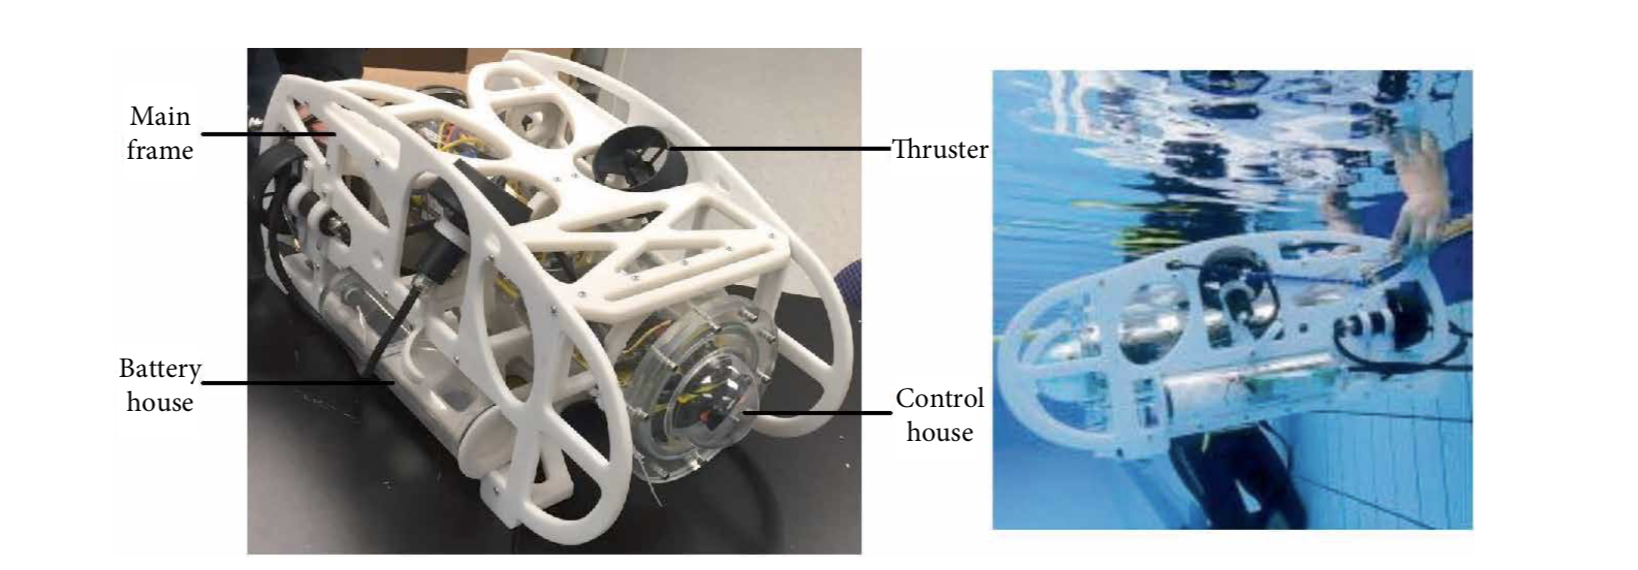
\includegraphics[scale=0.45]{figures/auv}
\caption{\small \sl Figuren viser roboten til Cui sitt team. Den kan detektere fisk og skal brukes til havforskning. \cite{Cui m.fl. 2020} \label{fig:auv}} 
\end{center} 
\end{figure} 

I 2020 så skrev Cui sitt team ``Fish Detection Using Deep Learning''. De jobber på en robot som kan utforske havet, se figur \ref{fig:auv}. I artikkelen deres dokumenterer de hvordan en lager en modell, et nevralt nettverk, som kan utføre fiskedeteksjon. De anvendte ``data augmentation'' teknikker. De brukte også Dropout algoritmen for å hindre at modellen ble overtilpasset, kjent som ``overfitting'' problemet. De endret også på loss funksjonen ettersom nettverket ble trent. Ved å bruke disse teknikkene så klarte de å redusere treningstiden og training loss. Systemet de lagde var optimalisert for et innebygd system, altså en svakere datamaskin, en AUV robot. \cite{Cui m.fl. 2020}

%\subsection{Perceptron}

%\subsection{Sigmoid neurons}
%%I teorikapitlet skal du plassere din studie inn i et overordnet teoretisk rammeverk. Formålet med dette kapitlet er å gjøre rede for de spesifikke teoriene og begrepene du anvender senere i avhandlingen. Du bør også begrunne hvorfor de er viktige for din studie. Du skal vise at du har forstått teorien du skal anvende. Pass på å bare skrive om det du bruker i analysen eller i tolkningen av datamaterialet.

%Det er verdt å merke seg at ikke alle oppgaver har en egen teoridel. Benytter du deg av IMRoD-modellen, har du presentert tidligere forskning i introduksjonen.

\section{Teori}

Machine Learning: Learning from data

Data is king.

Data collection, annotation, preporation etc.

Data > Algorithm > Training > Evaluation > Deployment > Predictions

	Gather data from every legal source possible (public data sets, purchase data, collect data, synthesize data (super poweful))

	Manually check data
	Look for biases
	Look for insights
	Clean up

	Iterative: Partition data 60 (training)/20 (testing accuracy training)/20 (test)

Model / Algorithm

	Image classification
	Object detection
	Segmentation

	Constraints

	Experimentation (test multiple viable models)

Training

	Data augmentation
	Training parameter (optimizer, rate etc.)
	Visualizsation (check if it is going correctly)

Evaluation

	Test. Check model size, speed and ACCURACY

Deployment

	Optimizations, deploy, feedback (know when it went badly, check failed images)

\subsection{Build your own}

Build your own:

1) Pick a state-of-the-art architecture

2) Make sure there is an open-source implementation

3) Make sure you get weights for this network trained on ImageNet


Experiment

1) Minimal architectural change
	Fine tune

2) If not enough: Tweak architecture
	More network blocks, new types of layers etc.

3) Search (Google's neural architecture search)

\subsection{resnet}

\begin{comment}
ResNet(
  (conv1): Conv2d(3, 64, kernel_size=(7, 7), stride=(2, 2), padding=(3, 3), bias=False)
  (bn1): BatchNorm2d(64, eps=1e-05, momentum=0.1, affine=True, track_running_stats=True)
  (relu): ReLU(inplace=True)
  (maxpool): MaxPool2d(kernel_size=3, stride=2, padding=1, dilation=1, ceil_mode=False)
  (layer1): Sequential(
    (0): Bottleneck(
      (conv1): Conv2d(64, 64, kernel_size=(1, 1), stride=(1, 1), bias=False)
      (bn1): BatchNorm2d(64, eps=1e-05, momentum=0.1, affine=True, track_running_stats=True)
      (conv2): Conv2d(64, 64, kernel_size=(3, 3), stride=(1, 1), padding=(1, 1), bias=False)
      (bn2): BatchNorm2d(64, eps=1e-05, momentum=0.1, affine=True, track_running_stats=True)
      (conv3): Conv2d(64, 256, kernel_size=(1, 1), stride=(1, 1), bias=False)
      (bn3): BatchNorm2d(256, eps=1e-05, momentum=0.1, affine=True, track_running_stats=True)
      (relu): ReLU(inplace=True)
      (downsample): Sequential(
        (0): Conv2d(64, 256, kernel_size=(1, 1), stride=(1, 1), bias=False)
        (1): BatchNorm2d(256, eps=1e-05, momentum=0.1, affine=True, track_running_stats=True)
      )
    )
    (1): Bottleneck(
      (conv1): Conv2d(256, 64, kernel_size=(1, 1), stride=(1, 1), bias=False)
      (bn1): BatchNorm2d(64, eps=1e-05, momentum=0.1, affine=True, track_running_stats=True)
      (conv2): Conv2d(64, 64, kernel_size=(3, 3), stride=(1, 1), padding=(1, 1), bias=False)
      (bn2): BatchNorm2d(64, eps=1e-05, momentum=0.1, affine=True, track_running_stats=True)
      (conv3): Conv2d(64, 256, kernel_size=(1, 1), stride=(1, 1), bias=False)
      (bn3): BatchNorm2d(256, eps=1e-05, momentum=0.1, affine=True, track_running_stats=True)
      (relu): ReLU(inplace=True)
    )
    (2): Bottleneck(
      (conv1): Conv2d(256, 64, kernel_size=(1, 1), stride=(1, 1), bias=False)
      (bn1): BatchNorm2d(64, eps=1e-05, momentum=0.1, affine=True, track_running_stats=True)
      (conv2): Conv2d(64, 64, kernel_size=(3, 3), stride=(1, 1), padding=(1, 1), bias=False)
      (bn2): BatchNorm2d(64, eps=1e-05, momentum=0.1, affine=True, track_running_stats=True)
      (conv3): Conv2d(64, 256, kernel_size=(1, 1), stride=(1, 1), bias=False)
      (bn3): BatchNorm2d(256, eps=1e-05, momentum=0.1, affine=True, track_running_stats=True)
      (relu): ReLU(inplace=True)
    )
  )
  (layer2): Sequential(
    (0): Bottleneck(
      (conv1): Conv2d(256, 128, kernel_size=(1, 1), stride=(1, 1), bias=False)
      (bn1): BatchNorm2d(128, eps=1e-05, momentum=0.1, affine=True, track_running_stats=True)
      (conv2): Conv2d(128, 128, kernel_size=(3, 3), stride=(2, 2), padding=(1, 1), bias=False)
      (bn2): BatchNorm2d(128, eps=1e-05, momentum=0.1, affine=True, track_running_stats=True)
      (conv3): Conv2d(128, 512, kernel_size=(1, 1), stride=(1, 1), bias=False)
      (bn3): BatchNorm2d(512, eps=1e-05, momentum=0.1, affine=True, track_running_stats=True)
      (relu): ReLU(inplace=True)
      (downsample): Sequential(
        (0): Conv2d(256, 512, kernel_size=(1, 1), stride=(2, 2), bias=False)
        (1): BatchNorm2d(512, eps=1e-05, momentum=0.1, affine=True, track_running_stats=True)
      )
    )
    (1): Bottleneck(
      (conv1): Conv2d(512, 128, kernel_size=(1, 1), stride=(1, 1), bias=False)
      (bn1): BatchNorm2d(128, eps=1e-05, momentum=0.1, affine=True, track_running_stats=True)
      (conv2): Conv2d(128, 128, kernel_size=(3, 3), stride=(1, 1), padding=(1, 1), bias=False)
      (bn2): BatchNorm2d(128, eps=1e-05, momentum=0.1, affine=True, track_running_stats=True)
      (conv3): Conv2d(128, 512, kernel_size=(1, 1), stride=(1, 1), bias=False)
      (bn3): BatchNorm2d(512, eps=1e-05, momentum=0.1, affine=True, track_running_stats=True)
      (relu): ReLU(inplace=True)
    )
    (2): Bottleneck(
      (conv1): Conv2d(512, 128, kernel_size=(1, 1), stride=(1, 1), bias=False)
      (bn1): BatchNorm2d(128, eps=1e-05, momentum=0.1, affine=True, track_running_stats=True)
      (conv2): Conv2d(128, 128, kernel_size=(3, 3), stride=(1, 1), padding=(1, 1), bias=False)
      (bn2): BatchNorm2d(128, eps=1e-05, momentum=0.1, affine=True, track_running_stats=True)
      (conv3): Conv2d(128, 512, kernel_size=(1, 1), stride=(1, 1), bias=False)
      (bn3): BatchNorm2d(512, eps=1e-05, momentum=0.1, affine=True, track_running_stats=True)
      (relu): ReLU(inplace=True)
    )
    (3): Bottleneck(
      (conv1): Conv2d(512, 128, kernel_size=(1, 1), stride=(1, 1), bias=False)
      (bn1): BatchNorm2d(128, eps=1e-05, momentum=0.1, affine=True, track_running_stats=True)
      (conv2): Conv2d(128, 128, kernel_size=(3, 3), stride=(1, 1), padding=(1, 1), bias=False)
      (bn2): BatchNorm2d(128, eps=1e-05, momentum=0.1, affine=True, track_running_stats=True)
      (conv3): Conv2d(128, 512, kernel_size=(1, 1), stride=(1, 1), bias=False)
      (bn3): BatchNorm2d(512, eps=1e-05, momentum=0.1, affine=True, track_running_stats=True)
      (relu): ReLU(inplace=True)
    )
  )
  (layer3): Sequential(
    (0): Bottleneck(
      (conv1): Conv2d(512, 256, kernel_size=(1, 1), stride=(1, 1), bias=False)
      (bn1): BatchNorm2d(256, eps=1e-05, momentum=0.1, affine=True, track_running_stats=True)
      (conv2): Conv2d(256, 256, kernel_size=(3, 3), stride=(2, 2), padding=(1, 1), bias=False)
      (bn2): BatchNorm2d(256, eps=1e-05, momentum=0.1, affine=True, track_running_stats=True)
      (conv3): Conv2d(256, 1024, kernel_size=(1, 1), stride=(1, 1), bias=False)
      (bn3): BatchNorm2d(1024, eps=1e-05, momentum=0.1, affine=True, track_running_stats=True)
      (relu): ReLU(inplace=True)
      (downsample): Sequential(
        (0): Conv2d(512, 1024, kernel_size=(1, 1), stride=(2, 2), bias=False)
        (1): BatchNorm2d(1024, eps=1e-05, momentum=0.1, affine=True, track_running_stats=True)
      )
    )
    (1): Bottleneck(
      (conv1): Conv2d(1024, 256, kernel_size=(1, 1), stride=(1, 1), bias=False)
      (bn1): BatchNorm2d(256, eps=1e-05, momentum=0.1, affine=True, track_running_stats=True)
      (conv2): Conv2d(256, 256, kernel_size=(3, 3), stride=(1, 1), padding=(1, 1), bias=False)
      (bn2): BatchNorm2d(256, eps=1e-05, momentum=0.1, affine=True, track_running_stats=True)
      (conv3): Conv2d(256, 1024, kernel_size=(1, 1), stride=(1, 1), bias=False)
      (bn3): BatchNorm2d(1024, eps=1e-05, momentum=0.1, affine=True, track_running_stats=True)
      (relu): ReLU(inplace=True)
    )
    (2): Bottleneck(
      (conv1): Conv2d(1024, 256, kernel_size=(1, 1), stride=(1, 1), bias=False)
      (bn1): BatchNorm2d(256, eps=1e-05, momentum=0.1, affine=True, track_running_stats=True)
      (conv2): Conv2d(256, 256, kernel_size=(3, 3), stride=(1, 1), padding=(1, 1), bias=False)
      (bn2): BatchNorm2d(256, eps=1e-05, momentum=0.1, affine=True, track_running_stats=True)
      (conv3): Conv2d(256, 1024, kernel_size=(1, 1), stride=(1, 1), bias=False)
      (bn3): BatchNorm2d(1024, eps=1e-05, momentum=0.1, affine=True, track_running_stats=True)
      (relu): ReLU(inplace=True)
    )
    (3): Bottleneck(
      (conv1): Conv2d(1024, 256, kernel_size=(1, 1), stride=(1, 1), bias=False)
      (bn1): BatchNorm2d(256, eps=1e-05, momentum=0.1, affine=True, track_running_stats=True)
      (conv2): Conv2d(256, 256, kernel_size=(3, 3), stride=(1, 1), padding=(1, 1), bias=False)
      (bn2): BatchNorm2d(256, eps=1e-05, momentum=0.1, affine=True, track_running_stats=True)
      (conv3): Conv2d(256, 1024, kernel_size=(1, 1), stride=(1, 1), bias=False)
      (bn3): BatchNorm2d(1024, eps=1e-05, momentum=0.1, affine=True, track_running_stats=True)
      (relu): ReLU(inplace=True)
    )
    (4): Bottleneck(
      (conv1): Conv2d(1024, 256, kernel_size=(1, 1), stride=(1, 1), bias=False)
      (bn1): BatchNorm2d(256, eps=1e-05, momentum=0.1, affine=True, track_running_stats=True)
      (conv2): Conv2d(256, 256, kernel_size=(3, 3), stride=(1, 1), padding=(1, 1), bias=False)
      (bn2): BatchNorm2d(256, eps=1e-05, momentum=0.1, affine=True, track_running_stats=True)
      (conv3): Conv2d(256, 1024, kernel_size=(1, 1), stride=(1, 1), bias=False)
      (bn3): BatchNorm2d(1024, eps=1e-05, momentum=0.1, affine=True, track_running_stats=True)
      (relu): ReLU(inplace=True)
    )
    (5): Bottleneck(
      (conv1): Conv2d(1024, 256, kernel_size=(1, 1), stride=(1, 1), bias=False)
      (bn1): BatchNorm2d(256, eps=1e-05, momentum=0.1, affine=True, track_running_stats=True)
      (conv2): Conv2d(256, 256, kernel_size=(3, 3), stride=(1, 1), padding=(1, 1), bias=False)
      (bn2): BatchNorm2d(256, eps=1e-05, momentum=0.1, affine=True, track_running_stats=True)
      (conv3): Conv2d(256, 1024, kernel_size=(1, 1), stride=(1, 1), bias=False)
      (bn3): BatchNorm2d(1024, eps=1e-05, momentum=0.1, affine=True, track_running_stats=True)
      (relu): ReLU(inplace=True)
    )
  )
  (layer4): Sequential(
    (0): Bottleneck(
      (conv1): Conv2d(1024, 512, kernel_size=(1, 1), stride=(1, 1), bias=False)
      (bn1): BatchNorm2d(512, eps=1e-05, momentum=0.1, affine=True, track_running_stats=True)
      (conv2): Conv2d(512, 512, kernel_size=(3, 3), stride=(2, 2), padding=(1, 1), bias=False)
      (bn2): BatchNorm2d(512, eps=1e-05, momentum=0.1, affine=True, track_running_stats=True)
      (conv3): Conv2d(512, 2048, kernel_size=(1, 1), stride=(1, 1), bias=False)
      (bn3): BatchNorm2d(2048, eps=1e-05, momentum=0.1, affine=True, track_running_stats=True)
      (relu): ReLU(inplace=True)
      (downsample): Sequential(
        (0): Conv2d(1024, 2048, kernel_size=(1, 1), stride=(2, 2), bias=False)
        (1): BatchNorm2d(2048, eps=1e-05, momentum=0.1, affine=True, track_running_stats=True)
      )
    )
    (1): Bottleneck(
      (conv1): Conv2d(2048, 512, kernel_size=(1, 1), stride=(1, 1), bias=False)
      (bn1): BatchNorm2d(512, eps=1e-05, momentum=0.1, affine=True, track_running_stats=True)
      (conv2): Conv2d(512, 512, kernel_size=(3, 3), stride=(1, 1), padding=(1, 1), bias=False)
      (bn2): BatchNorm2d(512, eps=1e-05, momentum=0.1, affine=True, track_running_stats=True)
      (conv3): Conv2d(512, 2048, kernel_size=(1, 1), stride=(1, 1), bias=False)
      (bn3): BatchNorm2d(2048, eps=1e-05, momentum=0.1, affine=True, track_running_stats=True)
      (relu): ReLU(inplace=True)
    )
    (2): Bottleneck(
      (conv1): Conv2d(2048, 512, kernel_size=(1, 1), stride=(1, 1), bias=False)
      (bn1): BatchNorm2d(512, eps=1e-05, momentum=0.1, affine=True, track_running_stats=True)
      (conv2): Conv2d(512, 512, kernel_size=(3, 3), stride=(1, 1), padding=(1, 1), bias=False)
      (bn2): BatchNorm2d(512, eps=1e-05, momentum=0.1, affine=True, track_running_stats=True)
      (conv3): Conv2d(512, 2048, kernel_size=(1, 1), stride=(1, 1), bias=False)
      (bn3): BatchNorm2d(2048, eps=1e-05, momentum=0.1, affine=True, track_running_stats=True)
      (relu): ReLU(inplace=True)
    )
  )
  (avgpool): AdaptiveAvgPool2d(output_size=(1, 1))
  (fc): Linear(in_features=2048, out_features=1000, bias=True)
)
\end{comment}
\subsection{Andrej Karpathy}

Andrej Karpathy (5,1 \%)

% Generellt

% Maskinsyn i matindustri

% Mitt arbeid

Sjømatdivisjonen og Akvadivisjonen ved Nofima har en strategisk internsatsing\footnote{\url{https://nofima.no/prosjekt/sameksistens/}} som går ut på å samle kunnskap om sameksistens mellom ulike marine næringer og interesser, deriblant om hvordan man kan unngå konflikter mellom ulike interesser. 

En av problemstillingene er sameksistens mellom fiskeri- og oppdrettsnæringene, og hvordan oppdrettsanlegg påvirker de nærliggende fiskeplassene. I den forbindelse er det interessant å kartlegge omfanget av hvitfisk som beiter på fôr fra oppdrettsanlegg. Dette er en problemstilling som har vært i fokus hos media\footnote{For eksempel \url{https://fiskeribladet.no/nyheter/?artikkel=69867} (hentet 12.02.2020)} etter at flere fiskere har fanget fôrsprengt torsk og sei i fjorder hvor det finnes oppdrettsanlegg. Det hevdes at denne fisken er av betydelig dårligere kvalitet og den kan ha fått i seg medisiner gjennom fôret som gjør at den kan være farlig å spise. 

Det behøves kunnskap om hvor mange villfisk som trekker til oppdrettsanlegg, og under hvilke forhold, slik at man kan komme nærmere en løsning som kan dempe konflikten mellom disse to næringene. 

\subsection{Mål}

Målet med dette prosjektet er å utvikle et system som kan telle antall villfisk av ulike arter basert på en videostrøm fra et undervannskamera. Det er ønskelig å kunne vise resultatet som en fordeling av observasjoner over tid for hver art. 
Til dette prosjektet er det anskaffet et undervannskamera av typen Steinsvik Orbit-3300 som styres via et MB-3000 kontrollpanel. Dette systemet er utviklet for inspeksjon av fisk i merd og tar opp data i form av en analog videostrøm. Denne kan sendes gjennom en analog-digital-omformer til en datamaskin hvor dataene til slutt vil kunne prosesseres i sanntid. 

\subsection{Delmål}

\subsubsection{Programvare skrevet i C++}

Prosjektet består i hovedsak av å utvikle en programvare som kan gjøre følgende ved hjelp av maskinlæring: 

\begin{enumerate}
\item Segmentere fisk fra bakgrunn
\item Klassifisere hver fisk etter art
\item Spore hver fisk gjennom hvert bilde i videostrømmen inntil fisken forlater kameraets synsfelt
\end{enumerate}

Programvaren implementeres i C++ ved hjelp av OpenCV-biblioteket\footnote{https://opencv.org/}. Det kan også være aktuelt å lage et grafisk grensesnitt hvor tellingene fra hver art kan vises i sanntid, men dette er avhengig av om prosjektets omfang tillater det. 

%\subsubsection{Praktisk del ved Havbruksstasjonen i Tromsø}

%Det er planlagt en praktisk del hvor kameraet skal plasseres ut på oppdrettsanlegg og samle data som kan prosesseres i ettertid for å teste programvaren. Dette blir mest sannsynlig på Havbruksstasjonen i Tromsø. Å finne beste plasseringen av kameraet i forhold til merdene er en viktig del av dette arbeidet med tanke på synsfelt og lysforhold. 

\subsubsection{Maskinsyn i matindustrien}

Nofima is a research organisation in the food industry

What about the salads and bama

The mathematics course had both calculus and optimization

You can explain about the tedious counting the salad leaves etc

Your data camera may do this

I can justify how computer vision is important in the food industry, and might revolutionize many industries

I can say this is a problem Nofima has, and wanted it solved with computer vision, as it is not only done before it is also cheaper than getting someone to manually count fish.

Say how you came to realise the importance doing practice at Bama, how you tried then to rig up a camera

There are already several players

You have marine robotics

And you have StingRay

The same with marine robotics

They use OpenCV and Qt

Mention that too lakselus very severe problem

I could also mention solving problems in an interesting way is the difference between drudgery and fun

And most problems are solved since they are interesting to someone

\section{Teori}

\subsubsection{Introduksjon til kunstig intelligens}

Dette er den offisielt første dagen av bacheloroppgaven. Den ble markert med en presentasjon av Sunniva Hoel, der hun presenterte blant annet innsida.ntnu.no/oppgaveskriving og tidligere bacheloroppgaver. Jeg fant en av dem, en litteraturgjennomgang som omhandlet matsvinn, på ntnuopen.ntnu.no.

Jeg avtalte med Stein-Kato på Nofima å møte ham tidlig mandag neste uke. Jeg skal være i Tromsø i to uker og jobbe på oppgaven, i uke 12 og 13.

Jeg har blitt ferdig med det første OpenCV kurset. Jeg har et kurs igjen, som handler om PyTorch, et deep convolutional neural network bibliotek. I løpet av det forrige kurset, lagde jeg en QR-kode leser, jeg lærte om ansiktsgjenkjenning (HAAR algoritmen) og folkemengdegjenkjenning (HOG algoritmen), jeg lagde chroma-keying (greenscreen) og kvisefjerningsprogammer, jeg implementerte algoritmer for noen morfologiske operasjoner som er typisk i maskinsyn fra scratch, jeg implementerte to forskjellige algoritmer som kameraer bruker til autofokus-egenskapen, jeg justerte fargelagene på bilder fra Sergey Prokudin-Gorsky, en klassisk fotograf fra tidlig 1900-tallet, og skal denne uken gjøre ferdig et prosjekt som handler om objektdeteksjon og tracking.

Jeg hadde problemer i går å få tracking, da spesifikt YOLOv3 tracking, til å virke med openCV på windows. I dag fant jeg ut at Visual Studio 2017 (vc15) støttes ikke helt av openCV lenger, og fikk tracking til å virke med Visual Studio 2019 (vc16).

I dag så gjorde jeg ferdig object deteksjon og object tracking prosjektet. Den bruker et dnn som heter YOLOv3, det er en modell som er trent til å gjenkjenne 80 forskjellige objekter. Blant dem er mennesker, bøker, vinglass osv. Det er fascinerende hvor enkelt det er å ta ibruk YOLO, og hvor godt den virker, selv om den ikke er perfekt. For tracking så brukte jeg KFC, en tracker som er implementert i openCV.

OpenCV er kun en inference engine, dvs. den kan kun gjøre "forward passes", eller eksekvere modeller, den kan ikke trene dem. For trening så må jeg ta ibruk PyTorch, som er det neste prosjektet. Ettersom YOLO ikke vet hva en fisk er, og i hvert fall ikke hva en torsk eller sei er, så må jeg trene en dnn selv. Det krever at jeg har mange bilder av fiskene. ImageNet er brukt at dataforskere til å trene netverk, men jeg finner ikke saith eller atlantic cod der. Så jeg får ta noen bilder selv i morgen av fisk fra frysedisken, og håpe at jeg får gode filmer og bilder i Tromsø av sei og torsk.

Jeg skal trene en supervised classification convolution network. Det vil si at jeg vil lære den opp ved å vise mange bilder av det jeg ønsker at den skal kjenne igjen, og noen eksempler på hva som ikke er det den skal vite om. Kunstige neurale nettverk lærer litt som barn. Det er viktig å vise så mange eksempler som mulig, og om en sier at noe er feil så må man være veldig sikker på at det faktisk er feil. Nettverket skal ha 3 outputs. Torsk, sei og ukjent.

Jeg så etter torsk og sei i dag i Trondheim. De selger kun fisk uten hode.

Prosjektet med YOLOv3 modellen må forbedres. Jeg lærte om kaggle.com, den har datasett for dataforskere. Den ser ikke ut til å ha fiskene heller.

Her er planen som alle Machine Learning oppgaver følger, "The ML Pipeline". Den består av følgende

\paragraph{Samling av data:} Kan gjøres på 4 måter.

A) Fra offentlige datasett med lovlige lisenser (kaggle.com, ImageNet osv.)
B) Kjøpe data
C) Samle data (Nofima Tromsø)
D) Syntesere data (Slik som 3D torsken som vi har)

\paragraph{Sjekke data}

A) Manuelt se igjennom dataen (lurt å se alle frames/bilder)
B) Se etter bias i bildene (f. eks, om bildene av fiskene inkluderer menneskehender, da kan modellen se etter ting på hendene på folk istedet for egenskapene til fisken)
C) Se etter innsikt (kan lære mye av å bare se på dataen)
D) Fiks opp dataen

\paragraph{Randomiser dataen}

\paragraph{Partisjoner dataen}

60 \% til trening av modellen
20 \% til å forbedre modellen (validation)
20 \% til testing (data modellen har aldri sett før)

Ettersom mennesker er late så er det mer vanlig med denne fordelingen:

80 \% trening
20 \% validation (test set)

\paragraph{Velg en algoritme eller modell}

Det finnes 3 typer problemer

Image classification
Object detection
Segmentation

\paragraph{Tenk på krav}

Presisjon
Hastighet
Plattform (mobil, windows, unix, GPU-server, osv.)

\paragraph{Eksperimenter}

Velg en modell, men prøv mange

\paragraph{Valg}

Velg en arkitektur og gjør prosjektet ferdig

I går så ble koronavirus offisielt betegnet som et pandemi av WHO, og Norge ble i dag "stengt". NTNU fraråder reise og campus er stengt for studenter. Stein-Kato har blitt satt i karantene da han har vært i Skottland denne uken. Jeg har avlyst turen til Tromsø. Jeg kommer til å fortsette å trene mine modeller på datasett som er tilgjengelige med PyTorch.

Jeg testet YOLOv3 på en syntetisk 3D torsk som vi har laget, YOLO har aldri sett en fisk før, og trodde det var en fugl. Nå får jeg mer tid på å lære PyTorch, det er egentlig veldig bra at jeg vet mer før jeg lager mitt eget datasett, så vet jeg bedre hva jeg burde gjøre når jeg er i Tromsø.

I dag så skulle jeg egentlig begynne reisen opp til Tromsø, men det ble avlyst pga. koronaviruset. Istedet så har jeg jobbet videre på PyTorch og objekt deteksjon og tracking programmet. Jeg har implementert ReLU, softmax og et kunstig neuron i Python, for å lære mer om hvordan PyTorch virker.

PyTorch er først og fremst rettet mot Python, og forskere og utviklere som foretrekker Python. De har laget et grensesnitt for C++ også. For å forstå PyTorch kreves det en forståelse av kalkulus, også kjent som funksjonsdrøfting, og lineær algebra. Vi hadde om kalkulus i kurset i første året, jeg kan noe lineær algebra fra forkurset, og universitetet jeg gikk på i Skottland.

Et kunstig neuron som anvendes i et neuralt nettverk ligner på ligningen til en linje.

\begin{equation}
y = ax + b
\end{equation}

Men den må være for flere dimensjoner.

\begin{equation}
y = w_i x + b
\end{equation}

Og X, som er input, kan også bestå av flere dimensjoner. Så en kan like gjerne representere w, weights (lagret i modellen) og input (x) med matriser. b er bias, og må lagres som en vektor.

\begin{equation}
y = WX + B
\end{equation}

Og that's it. I python blir dette

\begin{verbatim}
np.dot(W, X) + B
\end{verbatim}

Veldig enkelt.

\begin{figure} 
\begin{center} 
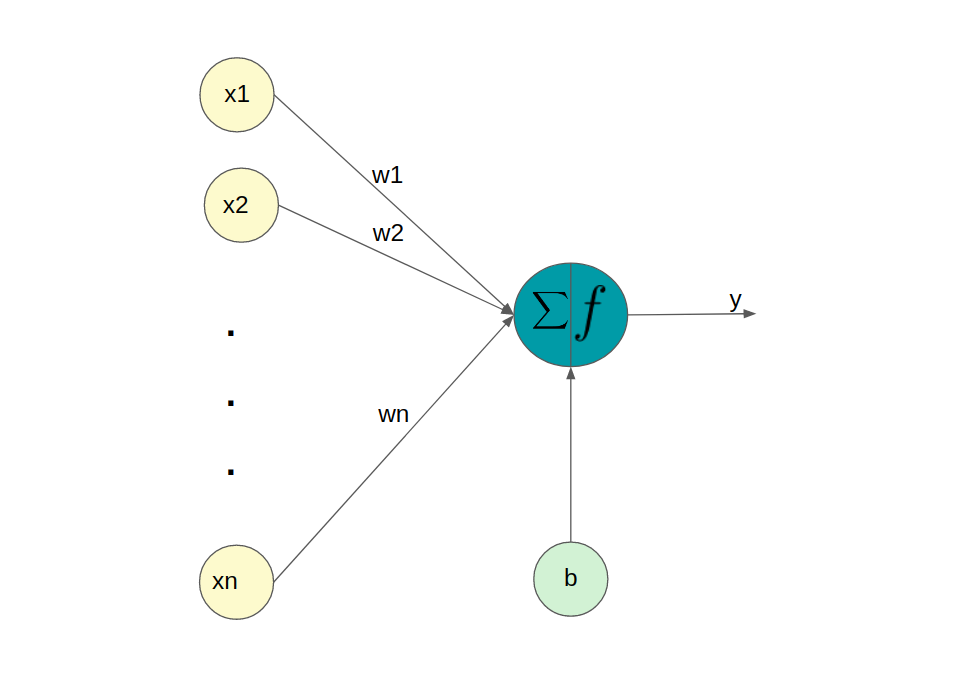
\includegraphics{figures/perceptron}
\caption{\small \sl Perceptron.\label{fig:perceptron}} 
\end{center} 
\end{figure} 

Jeg har implementert stochastic gradient descent i Python + PyTorch. Jeg har også laget nye implementasjoner av softmax, rectifier og kunstige neuroner i PyTorch.

Fordelen med PyTorch er at den er maskinvareakselerert. Det vi si at GPU-en gjør beregningene, ikke bare CPU-en.

GPU-er kommer fra dataspillindustrien. Alle datamaskiner i dag er heterogene, det vil si at de har både en CPU, en generell datahjerne, og en GPU, en grafikkdatahjerne. GPU-er er mange tusen ganger raskere enn en CPU, men kun for oppgaver som er "massively parallel". Både medisin, neurale nettverk, maskinsyn CAD, 3D animasjonsfilmproduksjon, spillutvikling og virtual reality drar nytte fra GPU-er.

Det er viktig i kunstig intelligens å vite hvor et datapunkt hører hjemme. Dette gjøres med kalkulus. Mange av problemene i kunstig intelligens, og maskinsyn, er optimaliseringsproblemer. Stokastic Gradient Descent (SGD) handler om å finne en linje som passer en modell. Det er matematisk optimalisering.

Jeg fikk vite om boken deeplearningboook.org , en gratis og svært god bok om deep learning. Elon Musk sier om boken: "Written by three experts in the field, Deep Learning is the only comprehensive book on the subject." (CEO SpaceX og Tesla)

Jeg har lært mye om deep learning i dag. Jeg har blitt tipset om http://cs231n.stanford.edu/ og http://playground.tensorflow.org/.

Som sagt så er de fleste maskinlæringsproblemer optimaliseringsproblemer. Det handler å finne ut hvor forskjellige datapunkter hører hjemme.

Det finnes flere forskjellige typer problemer. Katogerisering (gi navn på data inn) og regresjon (gi et tall ut fra data inn) er typiske.

Gamle neurale nettverk var perceptrons med lineære aktiveringsfunksjoner der en måtte gjøre features engineering per prosjekt for at modellen skulle virke. En kan leke med dette på tensorflow sin playground, aktiver inputs utover x1 og x2, fjern alle "hidden layers" og sett activation til linear. Test med forskjellig data. Den vil takle dataen som er i to godt avskilte skyer uten at en må tukle med features. Denne gamle måten å trene nettverkene (å finne parametere til activation featuren, for så å lage gode weights for modellen) krevde at en hadde god intuisjon om dataen en ønsket å trene nettverket på. Deep Learning med en ikke-lineær aktiveringsfunksjon gjør at den samme arkitekturen virker for alle problemer, uten feature engineering. Dette kan også lekes med, lag en eller to "hidden layers", fjern alle features untatt x1 og x2, og velg en ikke-lineær aktiveringsfunksjon. Vips, den takler alle data uten noen engineering/tweakkng, gitt nok neuroner. Tensorflow er Google sin rival til PyTorch, PyTorch er laget av Facebook.

PyTorch er delvis implementert i CUDA. Dette er en GPGPU-API som fungerer kun på Nvidia GPU-er. Jeg er mer interessert i Khronos sin OpenCL-standard, som er støttet av AMD, Nvidia, Intel, samt ARM og mange mobile GPU produsenter. Jeg får bruke PC-en i stua, som har en Nvidia-GPU, når jeg trener nettverket med PyTorch.

\begin{figure} 
\begin{center} 
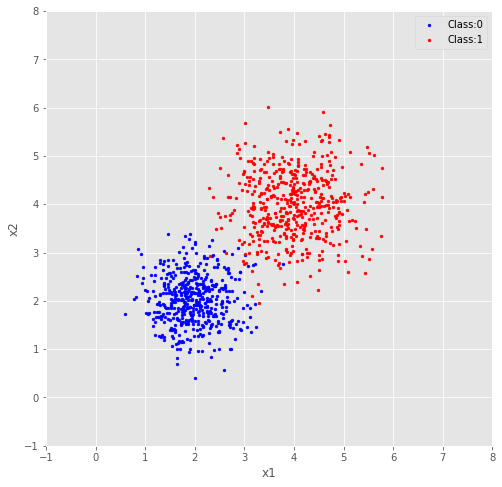
\includegraphics{figures/datapunkter}
\caption{\small \sl Eksempel av datapunkter. De består av to forskjellige klasser, vist i rødt og blått.\label{fig:datapoints}} 
\end{center} 
\end{figure} 

Se figur \ref{datapoints}. 

\begin{figure} 
\begin{center} 
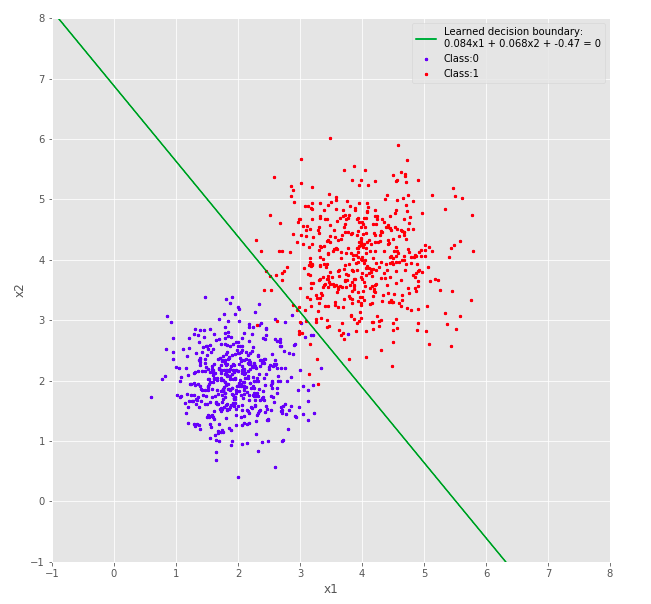
\includegraphics{figures/decision_boundary}
\caption{\small \sl Figuren over viser decision boundary. Det er dette ML handler om, å lage denne funksjonen som skiller dataen i to grupper, her binært til gruppe 0 og 1.\label{fig:datapoints}} 
\end{center} 
\end{figure} 

Jeg har begynt å trene opp en cnn. Jeg har en viss oversikt over deep learning nå. Det var i 2012 deep learning ble stort med AlexNet, de vant ImageNet med stor margin ved å finne på en ny måte å gjøre maskinlæring, det var deep learning.

Jeg har samlet en del whitepapers som jeg skal bruke i rapporten.

PyTorch har mange modeller. De har blitt veldig gode siden 2012, da måtte teamet til Geoffrey Hinton lage hele nettverket selv i CUDA. Nå er det veldig lett å lage programmer som kjenner igjen bilder med PyTorch. PyTorch gjør det også lett å laste ned test-data, og laste inn datasett, til å teste og trene modellen en velger.

Det er visstnok ikke lov ("de vil se stygt på deg") å si at et kunstig neuron er som et biologisk neuron. Det er litt som å si at et fly er som en fugl. Kunstige neuroner er lignende biologiske neuroner på samme måte som fly er inspirert av fugler. 

\begin{figure} 
\begin{center} 
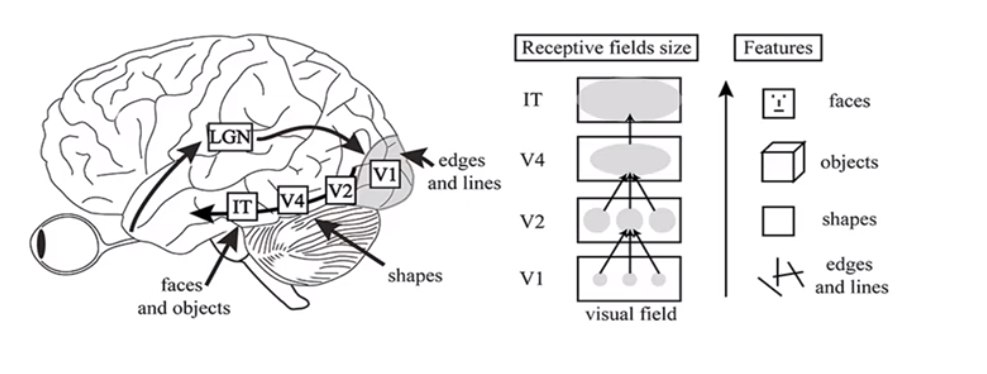
\includegraphics{figures/biological_inspiration_cnn}
\caption{\small \sl Den biologiske inspirasjonen for cnn.\label{fig:datapoints}} 
\end{center} 
\end{figure} 

\begin{figure} 
\begin{center} 
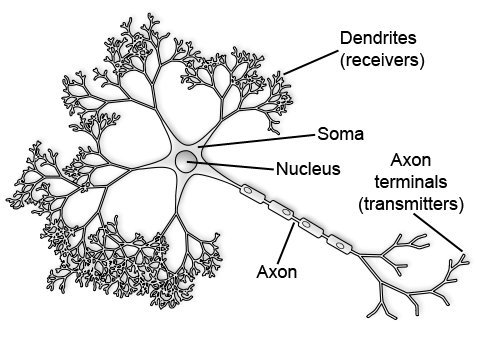
\includegraphics{figures/neuron_figure}
\caption{\small \sl Neuron\label{fig:datapoints}}
% https://commons.wikimedia.org/wiki/File:Neuron_figure.png
% Nicolas.Rougier 
\end{center} 
\end{figure} 

I dag trente jeg en ny modell og forbedret den jeg jobbet på Fredag. Denne modellen er trent med data fra PC-en min, av en panda, katt og hund. Det jeg gjorde i dag var bare en test på pipelinen og på at dataen lastes inn riktig. Jeg testet dermed kun 1 % av bildene i datasettet. Jeg fikk allikevel gode resultater. Da kan jeg gå videre.

Jeg fant mange gode whitepapers på deteksjon og tracking av fisk. Å google "fish detection" gir mange resultater fra mange forskjellige prosjekter. Det blir veldig nyttig for senere.

Treningen jeg skal gjøre er å lage en modell som ser forskjellen på torsk og sei. Jeg skal også lage et program som tracker og teller fisken. Å telle fisken er trivielt etter deteksjon. Dette er fine-grained detection. Jeg fant en whitepaper som tar opp spesifikt å detektere fisk av forskjellige fiskearter. Kanskje jeg låner ideer fra dem. Kan også prøve å trene deres datasett også for å få litt mer erfaring.

https://www.kaggle.com/ashishsaxena2209/animal-image-datasetdog-cat-and-panda

\url{https://www.researchgate.net/publication/317558591_Automatic_fish_species_classification_in_underwater_videos_Exploiting_pretrained_deep_neural_network_models_to_compensate_for_limited_labelled_data}

Steg 1 - Forstå problemet
Steg 2A - Få tak i data
Steg 2B - Utforsk og forstå dataen
Steg 2C - Lag et utvalg av dataen fra datasettet
Steg 3 - Gjør klar dataen
Steg 4 - Tren en enkel modell på datautvalget og test pipelinen før trening av et komplett nettverk påbegynnes
Steg 5 - Tren med et komplett datasett
Steg 6 - Iterativt forbedre modellen

I dag jobbet jeg på modellen. Jeg har testet den på datasei og datatorsk. Den klarer å se forskjellen på dem med 100 \% nøyaktighet. Jeg har enda ikke gjort ferdig modellen. Jeg må fortsatt trene hele modellen, så langt så har jeg gjort steg 1-4, jeg har steg 5-6 igjen. Den neste delen av oppgaven blir å bruke modellen til objekt deteksjon og tracking i en film, slik jeg gjorde med YOLOv3 modellen tidligere.

Jeg skal lage et nytt datasett med ekte torsk og sei.

\begin{figure} 
\begin{center} 
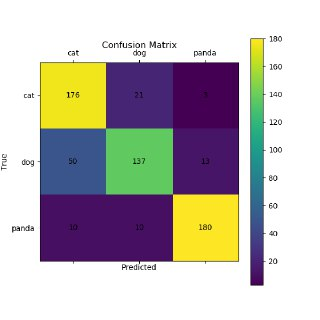
\includegraphics{figures/confusion_matrix}
\caption{\small \sl Forvirringsmatrise. n*n. Den vil vise falske positive, sanne positive, falske negative og sanne negative for hver klasse. Om denne cnn-en var for å detektere brystkreft, og positivt sykdom betyr at en kvinne har brystkreft, så hadde falske positive vært ganske dårlig, og falske negative vært katastrofalt. En modell som, for eksempel, sier negativ hele tiden vil være 95 \% riktig, da bryskreft skjer sjeldent (i 5 \% av tilfellene, i dette tilfellet). Bias er farlig, det er viktig å balansere dataen sendt til en modell. Like mye data per klasse. \label{fig:datapoints}}
\end{center} 
\end{figure} 

I dag implementerte jeg step-wise learning decay til modellen i et forsøk på å få bedre nøyaktighet. En modell skal ha høy learning rate i begynnelsen, så skal den bli mindre for å nå bunnen av læringskurven.

Videre, å detektere fisk med maskinsyn har blitt gjort før. Det er mye bra som er skrevet om dette.

Vi diskuterte hva som har gjort deep learning så populært den siste tiden. Her er nye fremskritt de siste 10 årene som har gjort deep learning populært (LeNet vs AlexNet, Andrej Karpathy 2020)

\begin{figure} 
\begin{center} 
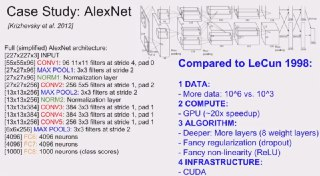
\includegraphics{figures/alexnet}
\caption{\small \sl Vi diskuterte hva som har gjort deep learning så populært den siste tiden. Her er nye fremskritt de siste 10 årene som har gjort deep learning populært (LeNet vs AlexNet, Andrej Karpathy 2020) \label{fig:datapoints}}
\end{center} 
\end{figure} 

Jeg har fått til YOLOv3 nå. Den går mye raskere enn RetinaNet, og kan gå i sanntid med en Nvidia GPU, slik som en 2070 gtx (regner jeg med).

Jeg har brukt dagen på å se på tracking. Den må tracke flere objekter, det betyr flere trackere. En tracker krever ganske mye fra CPU-en. Det gjør programmet saktere. Men de kan multithreades. Jeg har enda ikke klart å gjøre alle fiskene som blir detektert til noe som trackes. Tracking skal være raskere enn objektdeteksjon. Jeg kan gjøre deteksjon sjeldnere enn tracking, slik at programmet går raskere. Men det må fortsatt testes. Deteksjon må uansett skje med jevne mellomrom, da nye kommer stadig inn i i bildet.

Jeg har laget flere masks for segmentering, som blir et siste eksperiment, etter YOLOv3 er trent opp på sei og tracking er blitt eksperimentert med.

Jeg snakket med Nofima i dag. Jeg forklarte arbeidet som jeg har gjort. Vi ble enige om å se litt mer på tracking, jeg forklarte at deteksjon uten tracking vil nok virke like bra.

I dag lastet jeg opp realeases av app på github. Stein-Kato har tilgang til prosjektet nå. Jeg håper han får brukt arbeidet.

Jeg har begynt å se på segmentering. Jeg håper å bli med på to kaggle konkurranser i løpet av måneden. Jeg har begynt å tenke mer på rapporten, skrivingen får nesten begynne for fullt nå, så stiller jeg bedre forberedt til BO-seminaret den 30. April.

\subsubsection{Maskinlæring}

Machine Learning: Learning from data

Data is king.

Data collection, annotation, preporation etc.

Data > Algorithm > Training > Evaluation > Deployment > Predictions

	Gather data from every legal source possible (public data sets, purchase data, collect data, synthesize data (super poweful))

	Manually check data
	Look for biases
	Look for insights
	Clean up

	Iterative: Partition data 60 (training)/20 (testing accuracy training)/20 (test)

Model / Algorithm

	Image classification
	Object detection 
	Segmentation

	Constraints

	Experimentation (test multiple viable models)

Training

	Data augmentation
	Training parameter (optimizer, rate etc.)
	Visualizsation (check if it is going correctly)

Evaluation
	
	Test. Check model size, speed and ACCURACY

Deployment

	Optimizations, deploy, feedback (know when it went badly, check failed images)	

\subsubsection{Neural networks}

Classification (Supervised learning)

	Seperating data into groups

	Binary classification (two groups) (Sigmoid activation is used)

	Multiclass classification (Activation: Softmax) (Loss function: Cross entropy loss)

	Regression (Activation: Linear) (Loss function: MSE loss)

	Decision boundary seperates the groups by the decision function

	Training is learning the decision function

	Deciding decision function is called training

	Data is on a plane (2D) or a hyperplane (higher dimensions)

	Input layer > Hidden layer (can be many layers) > output

	Each layer (node) in a nn is a neuron or perceptron

	Perceptron: Calculate weighted sum of inputs and add bias. Then apply activation function (non-linear)

	Every layer looks for a pattern found in the previous layer. If it is found, it "fires up"

	An example of an activation function is ReLU (Rectified Linear Unit)

	Another example is the sigmoid function, and tanh

	An activation function creates non-linearity

	The number of hidden layers is called the networks depth (depth = 2 is typical for simple problems)

Loss functions

	Classification outputs a category (class)

	Regression outputs numerical values (or a vector of numerical values)

	Many problems are optimizatino problems in ML, either to minimize or maximaze a value of a function

	These functions are called the objective function

	When finding the minimum, it is called a loss, or cost, function

	e = y - \^y (error is ground thruth minus model output)

	An error, L, can be considered either a square (MSE, most common) or an absolute number (MAE, when data has many outliers)

Single layer perceptron kan løse lineære problemer

Ved å gjøre "feature engineering" så kan ikke-lineære problemer løses

Deep learning gjør at en kan løse lineære problemer om en bruker ikke-lineær aktivering. ReLU konvergerer raskt.

\subsubsection{Maskinsyn med OpenCV}
\subsubsection{Video med undervannskamera fra merdene}
\subsubsection{Analysere video}
\subsubsection{Deep Learning med OpenCV}
\subsubsection{PyTorch}
\subsubsection{Segmentere ut fisk}
\subsubsection{Object Detection med OpenCV}
\subsubsection{Object Tracking med OpenCV}
\subsubsection{Klassifisere hver fisk etter art}
\subsubsection{Registrere antall individer av hver art fortløpende}
\subsection{Praktisk gjennomføring}
\subsubsection{Programvareutvikling med maskinlæring implementert i C++}
\subsubsection{Videostrøm fra merdene}
\subsection{Resultater}
\subsection{Diskusjon}
\subsection{Konklusjon}
\subsection{Referanseliste}

% Materialer og metoder 2/5
%I dette kapitlet skal du skrive om hvordan du har gått frem metodisk, og vise hvordan valg av design og metode egner seg til å svare på problemstillingen din.

%Kapitlet må kunne gi svar på disse spørsmålene:

%Hvordan samlet du inn datamaterialet?
%Hvordan behandlet du dataene du samlet inn?
%Hvorfor valgte du disse metodene?
%Hva er styrkene og svakehetene ved disse metodene?
%Du skal også si noe om hvorfor du har gjort din undersøkelse på den måten du gjorde – og da peke på styrker og svakheter. I tillegg skal du drøfte etiske aspekter ved prosjektet. På den måten viser du at du har kommet frem til resultatene på en pålitelig og troverdig måte, men også at du er reflektert og kritisk overfor arbeidet du har gjort.

%Husk også at du her, slik som i teorikapitlet, bare skal skrive om det metodiske som er relevant for din studie.
\section{Metode}

\begin{figure}[h!]
\begin{center} 
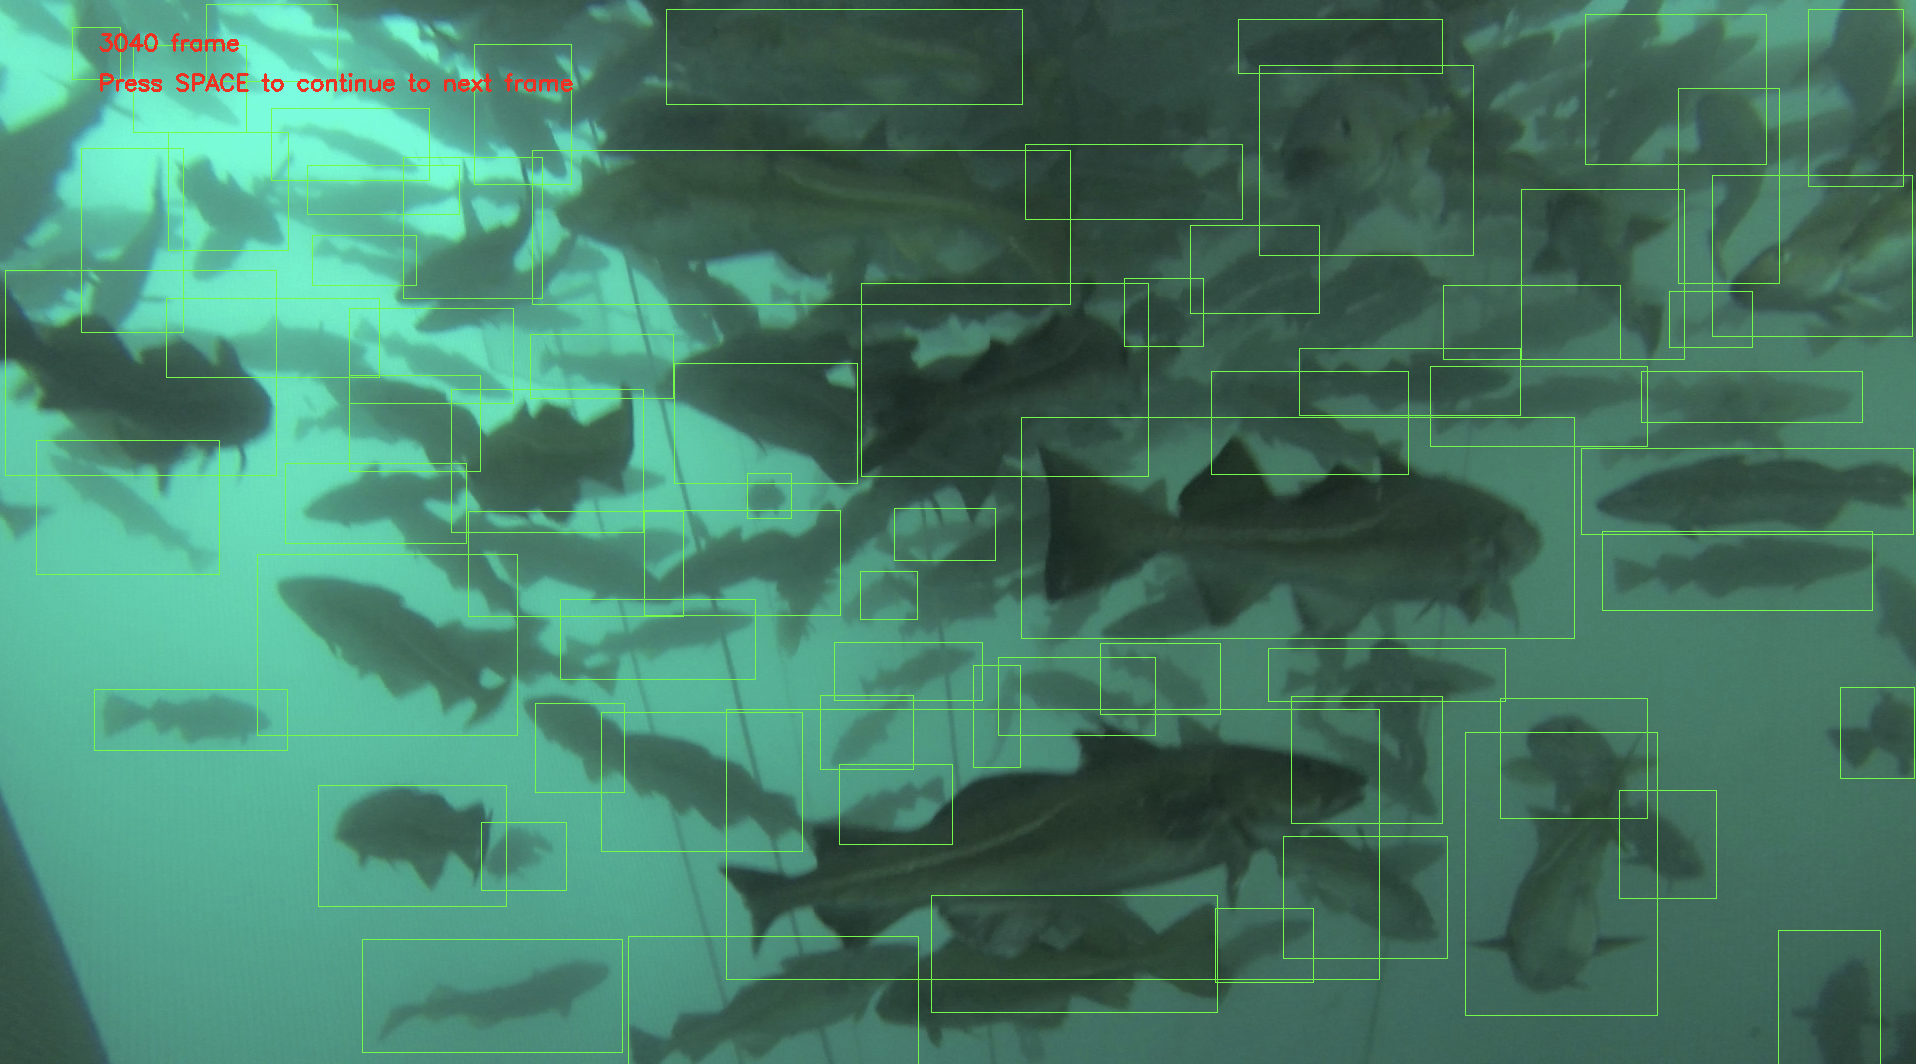
\includegraphics[scale=0.35]{figures/dataset_tool_2}
\caption{\small \sl Figuren viser et dataprogram som ble utviklet for å lage label data basert på opptakene fra Nofima. Dataprogrammet laster inn hvert femtiende bilde fra en video av en lagringsmerd av torsk. Denne videoen er 7 minutter lang. På figuren vises bilde nummer 3040. En modell som kan detektere objekter krever å bli trent på bilder av det den skal kjenne igjen, bilder med label data. Label data består av klassenummer, og `xmin', `ymin', `xmax', og `ymax' posisjoner, som skaper et rektangel rundt objektene som finnes i bildet, for hvert objekt som finnes i treningsdataen. Med dette dataprogrammet så er å lage slik informasjon fra et bilde enkelt, brukeren trenger kun å lage et rektangel rundt hver torsk. Klassenummeret for torsk, her 0, og posisjonene av rektangelet, `xmin', `ymin', `xmax', og `ymax', kjent som objektets ground truth bounding box, lagres til en tekstfil. Rådataen, bilde uten rektanglene eller den røde teksten som er øverst i venstre hjørne, lagres også automatisk til en mappe. \label{fig:dataset_tool}} 
\end{center} 
\end{figure} 

%Dette kapitlet er obligatorisk for alle forsøksoppgaver. Det bør innledes med et flytskjema/oversikt og en beskrivelse som letter leserens forståelse av hva som er gjort. Dette gjelder både for rene analyseoppgaver og for produktutviklingsoppgaver. 

%Beskrivelsen av materialer og metoder skal være tilstrekkelig detaljert slik at andre kan vurdere arbeidet og om ønskelig gjenta forsøkene. Samtidig må man unngå å fylle opp rapporten med unødige detaljer. Dersom det er brukt en velkjent metode, er det nok å bruke metodens offisielle navn og henvise til offisiell kilde. Hvis det var nødvendig med modifikasjoner eller andre tilpasninger i forhold til metoden, må dette beskrives. Eventuell teori om metoden, hører hjemme i teoridelen. Beskriv det dere har gjort og ikke det dere skulle ha gjort. 

%Hensikten med kapitlet Materialer og metoder er at andre skal kunne utføre det samme arbeidet på samme måte. Da må alle nødvendige opplysninger være med.

Trening av kunstige nevrale nettverk gjøres i seks steg. Det ble trent opp to modeller, en RetinaNet modell og en YOLOv4 modell. RetinaNet hadde forhåndstrente vekter fra en modell trent på COCO datasettet til Microsoft, og YOLOv4 hadde fohåndstrente vekter fra en modell trent på ImageNet datasettet, modellene ble ikke trent fra scratch. %You should design a model which achieves 85 \% validation accuracy on the given dataset.

Microsoft Azure plattformen ble anvendt til å trene modellene. Microsoft tilbyr Nvidia Titan GPU-er i skyen. Å anvende GPU-er når en trener kunstige nevrale nettverk gjør at treningen tar mindre tid.

Det tok ca. 2 dager å trene YOLOv4 modellen på nettskyen Azure med maskinstørrelsen Standard NC6 Promo (6 vcpu-er, 56 GiB dataminne). Trening av RetinaNet tok mye mindre tid, men inferens av RetinaNet tok over seks timer for 7 minutter video. YOLOv4 kan gjøre inferens på noen millisekunder per bilde, der RetinaNet bruker titals sekunder selv på kraftig maskinvare.% Se figur retinanet vs YOLOv4 resultater

Kildekoden for prosjektet kan lastes ned fra: \\ \url{https://github.com/alanhaugen/TMAT3004-Bacheloroppgave}.

\subsection{Å forstå problemet}

Før en begynner så er det viktig å være sikker på at man forstår problemet en skal løse. I denne oppgaven så skulle mengden av to fisk, torsk og sei, telles med maskinsyn. Det er to klasser. For å løse denne oppgaven kreves bilder av hver fisk med korrekt label-data og et rimelig stort nettverk som kan forstå og trenes på bilder.

Objektdeteksjon handler om to ting. Områder av bilde som kan inneholde en klasse må genereres, og så må disse delene av et bilde klassifiseres basert på det visuelle innholdet i bildeområdet, et bildeområde kalles for en patch innenfor maskinsyn. Områdene der det kan være objekter kalles for ankre. Med andre ord, målet for modellen er å se på en del av et bilde og finne ut hvilket objekt som finnes i dette området. Nettverket kan kun finne de objektene som den har blitt trent til å gjenkjenne.

\subsection{Få tak i data}

Det neste steget var å få tak i data. Datasettet som ble laget for dette prosjektet bestod av bilder fra en lagringsmerd av torsk, og bilder av sei fra Havbruksstasjonen i Tromsø. Se figur \ref{fig:data} og \ref{fig:nofima}. Opptakene av fiskene ble laget av Nofima og ble omgjort til bilder. Label data lagt inn manuelt. Se figur \ref{fig:dataset_tool}. Dataen av torsk var fargebilder, så de bestod av tre kanaler, og hadde størrelsen 1920 $\times$ 1080. %You need to achieve 85 \% accuracy for validation data to successfully complete this assignment. Check it out here.

\begin{figure}[h!]
\begin{center} 
\includegraphics[scale=0.05,angle=-90,origin=c]{figures/camera_1}
\includegraphics[scale=0.05,angle=-90,origin=c]{figures/camera_2}
\includegraphics[scale=0.05]{figures/camera_3}
\caption{\small \sl Figuren viser kamerautstyret som ble anvendt til å lage seidataen. Nofima anskaffet et undervannskamera av typen Steinsvik Orbit-3300 som styres via et MB-3000 kontrollpanel. \label{fig:nofima}} 
\end{center} 
\end{figure} 

Datasettet bestod av 208 bilder av torsk, med til sammen 4582 instanser av torsk i bildene. Det var (--) bilder av sei med (--) instanser av fisken i bildene. Bildene av torsk og sei ble satt i hver sin mappe. De ble splittet etter forholdet 80/20, 80 \% av dataen var for trening, og 20 \% for validering.

\subsubsection{Utforsk og forstå dataen}

Det er viktig å se på dataen før en begynner å trene et nettverk. Det er viktig å se etter bias i bildene. Det er lurt å gå igjennom hvert eneste bilde, og se om det er noe en kan lære. Torsk og sei bildene kunne bli augmented, de kunne blant annet bli snudd horisontalt. Det gir dobbelt så mye treningsdata. Vær obs på at ikke alle treningssett tillater dette, for eksempel et datasett med lego.

Det var to klasser i datasettet, torsk og sei. Se figur \ref{fig:tree} og tabell \ref{tab:classes}.

\begin{figure}[h!]
\Tree[.data [.labels ] [.train [.atlantic\_cod ]
               [.saithe ]]
          [.validation [.atlantic\_cod ]
                [.saithe ]]]
\caption{\small \sl Figuren viser et tre av mappestrukturen til datasettet. \label{fig:tree}} 
\end{figure} 

\begin{table}[h!]
\bigskip
\centering
\caption{Klassenavn og navneenkoding for datasettet}
\label{tab:classes} 
\begin{tabular}[t]{lcc}
\toprule
Klassekode & Klassenavn    & Norsk klassenavn \\
\midrule
0          & atlantic\_cod & torsk            \\
1          & saithe        & sei         \\
\bottomrule	
\end{tabular}
\end{table}

`Labels` mappen inneholdt bounding box data for bildene. Det var en eller flere linjer per `.txt` fil. Hver linje representerer en bounding box. Representasjonen er i `xmin', `ymin', `xmax', og `ymax' formatet. Se tabell \ref{tab:bbox}.

Filene som ble brukt til trening og validering ble definert i \url{data/fish_train.txt} og \url{data/fish_test.txt}. Se tabell \ref{tab:fish}.

\begin{table}[b]
\bigskip
\centering
\caption{Label data for bilde \url{data/train/atlantic_cod/fish_9440.png}, lagt i fil \url{data/labels/fish_9440.txt}}
\label{tab:bbox} 
\begin{tabular}[t]{lcccc}
\toprule
Klassekode    & xmin      & ymin    & xmax     & ymax \\
\midrule
0 & 238 & 643 & 582 & 882 \\
0 & 80   & 858 & 368 & 1071 \\
\bottomrule	
\end{tabular}
\end{table}

\begin{table}[b]
\bigskip
\centering
\caption{Eksempel på filnavn i \url{data/fish_train.txt} og \url{data/fish_test.txt}}
\label{tab:fish} 
\begin{tabular}[t]{c}
\toprule
Filnavn i \url{fish_test.txt} \\
\midrule
\url{validation/atlantic_cod/fish_590.png} \\
\url{validation/atlantic_cod/fish_640.png} \\
\vdots \\
\bottomrule	
\end{tabular}
\end{table}

\subsection{Gjør klar dataen}

Da dataen hadde blitt organisert, og label data nøye konstruert, så ble nettverkene konfigurert og treningen ble satt i gang. Dataen ble matet inn i treningsprogrammet, inn i deep learning rammeverkene.

Det ble trent opp to nettverk. Den ene, RetinaNet, er en del av detectron2 fra Facebook. Den ble trent og konfigurert med PyTorch. Den andre modellen var YOLOv4, den trenes med deep learning rammeverket darknet. Konfigurasjon gjøres ved å endre på tekstfiler og kommandolinjeparameterene til rammeverket.

\subsubsection{Dataaugmentering}

Dataen må først normaliseres på en standard måte, for eksempel ved å subtrahere gjennomsnittet over dataen, for så å skalere alle bildene slik at de får samme størrelse. Det er også mulig å gjøre flere andre endringer. Støy kan legges til bildene, samt å snu dem horisontalt eller vertikalt for å skape nye bilder å trene nettverket på.

Det ble ikke gjort endringer på standardmåten detectron2 og darknet gjør dataaugmentering.

\subsubsection{YOLOv4 label data og bildeformat}

YOLOv4 har et annet label-format sammenlignet med RetinaNet, dessuten krever den bilder i jpeg formatet, med filudvidelsen .jpg. Label-dataen legges sammen med bildene. Konvertering fra RetinaNet sitt format til YOLOv4 ble gjort med et awk-skript. Formatet til YOLOv4 er:

\begin{verbatim}
[klassenavn] [objekt midtpunkt i X] [objekt midtpunkt i Y]
	[objekt vidde i X] [objekt høyde i Y]
\end{verbatim}

Et nyttig verktøy til å konvertere bilder er John Cristy sin Image Magick. Her er hvordan bildene ble konvertert fra Adobe sitt png format til jpeg:

\begin{verbatim}
mogrify -format jpg *.png
\end{verbatim}

\subsection{Tren nettverket på et lite utvalg av dataen som en test før en trener et fullt nettverk}

Nettverket ble først trent opp på et utvalg av treningsdataen, for å teste nettverket. 208 bilder med 4582 instanser av torsk ble grunnlaget for de første RetinaNet og YOLOv4 modellene. Dette steget gjøres som en sanity check før en begynner på trening som kan ta mange timer.

RetinaNet modellen ble trent med en learning rate på 0,001 over 500 iterasjoner. Modellen brukte vekter fra COCO, den ble lastet ned fra the model zoo, den heter \url{COCO-Detection/retinanet_R_50_FPN_3x.yam}. RetinaNet sin score threshold ble satt til 0,5. Batch size var 4.

\subsubsection{RetinaNet konfigurasjon og trening}

RetinaNet er implementert i detectron2, som bruker deep learning rammeverket PyTorch. Grensesnittet er programmeringsspråket Python. Detectron2 er utgitt under en Apache 2.0 lisens, det vil si at den kan brukes til hva enn en vil på en hvilken som helst måte, gratis, så lenge man aksepterer at facebook ikke blir ansvarlig for arbeidet som gjøres, og så lenge man ikke krediterer arbeidet en gjør til facebook \cite{The Apache Software Foundation 2004}. Detectron2 installeringsinstrukser er tilgjengelig her: \url{https://detectron2.readthedocs.io/}

Først må bibliotekene lastes inn. Se python koden under.

\begin{lstlisting}[language=Python, caption=Her lastes bibliotekene inn i train.py for detectron2]
import torch
import detectron2
#import onnx
#from detectron2 import export
from detectron2.utils.logger import setup_logger
setup_logger()

# import some common libraries
import numpy as np
import cv2
import random
import os
import matplotlib.pyplot as plt

# model_zoo has a lots of pre-trained model
from detectron2 import model_zoo


# DefaultTrainer is a class for training object detector
from detectron2.engine import DefaultTrainer
# DefaultPredictor is class for inference
from detectron2.engine import DefaultPredictor

# detectron2 has its configuration format
from detectron2.config import get_cfg
# detectron2 has implemented Visualizer of object detection
from detectron2.utils.visualizer import Visualizer

# from DatasetCatalog, detectron2 gets dataset and from MetadatCatalog it
# gets metadata of the dataset
from detectron2.data import DatasetCatalog, MetadataCatalog

# BoxMode support bounding boxes in different format
from detectron2.structures import BoxMode

# COCOEvaluator based on COCO evaluation metric, inference_on_dataset is used for
# evaluation for a given metric
from detectron2.evaluation import COCOEvaluator, inference_on_dataset

# build_detection_test_loader, used to create test loader for evaluation
from detectron2.data import build_detection_test_loader

\end{lstlisting}

Konfigurasjonen defineres i neste kodesnutt.

%\begin{lstlisting}[language=Python, caption=Treningen og testingen, samt operativssystemet konfigureres]
\begin{lstlisting}[language=Python, caption=Konfigurasjon i train.py]
data_root = 'data'
train_txt = 'fish_train.txt'
test_txt  = 'fish_test.txt'

train_data_name = 'fish_train'
test_data_name  = 'fish_test'

thing_classes = ['atlantic_cod', 'saithe']

output_dir = 'outputs'

def count_lines(fname):
    with open(fname) as f:
        for i, l in enumerate(f):
            pass
    return i + 1

train_img_count = count_lines(os.path.join(data_root, train_txt))

# Register train and test data
# dataset can be registered only once with one name

# register train data
DatasetCatalog.register(name=train_data_name,
                        func=lambda: get_fish_dicts(data_root, train_txt))
train_metadata = MetadataCatalog.get(train_data_name).set(thing_classes=thing_classes)

# register test data
DatasetCatalog.register(name=test_data_name,
                        func=lambda: get_fish_dicts(data_root, test_txt))
test_metadata = MetadataCatalog.get(test_data_name).set(thing_classes=thing_classes)

# default configuration
cfg = get_cfg()

# update configuration with RetinaNet configuration
cfg.merge_from_file(model_zoo.get_config_file("COCO-Detection/retinanet_R_50_FPN_3x.yaml"))
cfg.MODEL.ROI_HEADS.SCORE_THRESH_TEST = 0.5

# We have registered the train and test data set with name fish_train and fish_test.
# Let's replace the detectron2 default train dataset with our train dataset.
cfg.DATASETS.TRAIN = (train_data_name,)

# No metric implemented for the test dataset, we will have to update
# cfg.DATASET.TEST with empty tuple
cfg.DATASETS.TEST = ()

# data loader configuration
cfg.DATALOADER.NUM_WORKERS = 4

# Update model URL in detectron2 config file
cfg.MODEL.WEIGHTS = model_zoo.get_checkpoint_url("COCO-Detection/retinanet_R_50_FPN_3x.yaml")
model_final_f10217.pkl"
\end{lstlisting}

Konfigurasjonen av batch size, data path og learning rate er de viktigste variablene, det er det neste som settes her. 

\begin{lstlisting}[language=Python, caption=Solver konfigurasjon i train.py]
# batch size
cfg.SOLVER.IMS_PER_BATCH = 4

# choose a good learning rate
cfg.SOLVER.BASE_LR = 0.001

# We need to specify the number of iteration for training in
# detectron2, not the number of epochs.
# lets convert number of epoch to number or iteration (max iteration)

epoch = 1000
max_iter = int(epoch * train_img_count / cfg.SOLVER.IMS_PER_BATCH)
max_iter = 500

cfg.SOLVER.MAX_ITER = max_iter

# number of output class
cfg.MODEL.RETINANET.NUM_CLASSES = len(thing_classes)

# update create ouptput directory
cfg.OUTPUT_DIR = output_dir
os.makedirs(cfg.OUTPUT_DIR, exist_ok=True)

\end{lstlisting}

Neste kodesnutt er trening, resultatene finnes på tensorboard: \\
\url{https://tensorboard.dev/experiment/aZzjBUzKTAy19KPsDZPJ2g}

\begin{lstlisting}[language=Python, caption=Treningskode i train.py]
# Create a trainer instance with the configuration.
trainer = DefaultTrainer(cfg) 

# if rseume=False, because we don't have trained model yet. It will
# download model from model url and load it
trainer.resume_or_load(resume=False)

# start training
trainer.train()

\end{lstlisting}

%You need to set up the training pipeline with a batchsize of 4 and run the experiment for 100 epochs. Make these changes in the Configrations given below.

\subsubsection{YOLOv4 trening}

Alexey Bochkovskiy sin fork av darknet ble anvendt, det er en versjon av Joseph Redmon sin Darknet: Open Source Neural Networks in C med Windows og Linux støtte. Den støtter nyere versjoner av OpenCV og det som var den nyeste versjonen av YOLO da denne rapporten ble skrevet, YOLOv4, som ble utgitt 23. April \cite{Bochkovskiy m.fl. 2020}. En god guide til darknet og YOLO finnes på githuben til Alexey. \cite{Bochkovskiy 2020}

cuDDN ble installert etter Nvidia sine instrukser. \url{https://docs.nvidia.com/deeplearning/sdk/cudnn-install/index.html#installlinux-tar}

YOLOv4 ble trent med vekter fra en forhåndstrent modell. Først må darknet installeres. Se under.

\begin{verbatim}
git clone https://github.com/AlexeyAB/darknet
cd darknet
\end{verbatim}

Omgjør linjene GPU=0, CUDNN=0, og OPENCV=0 og til GPU=1, CUDNN=1 og OPENCV=1 i Makefile.

\begin{lstlisting}[language={}, caption=De første linjene i Makefile]
GPU=1
CUDNN=1
CUDNN_HALF=0
OPENCV=1
AVX=0
OPENMP=0
LIBSO=0
ZED_CAMERA=0 # ZED SDK 3.0 and above
ZED_CAMERA_v2_8=0 # ZED SDK 2.X
\end{lstlisting}

Kompiler rammeverket.

\begin{verbatim}
make
\end{verbatim}

Dette vil kompilere darknet for GPU-en med OpenCV støtte.

%For å aktivere GPU-støtte, som vil gjøre treningen mye raskere om en har en Nvidia GPU med nok minne, settes GPU = 1 i Makefile-en, deretter rekompileres rammeverket. Rammeverket rekompileres ved å skrive make clean etterfulgt av make.

For å få gode resultater så ble forhåndstrente vekter for de convolutional lagene lastet ned. Den forhåndstrente darknet modellen (162 MiB) kan lastes ned her: \url{https://github.com/AlexeyAB/darknet/releases/download/darknet_yolo_v3_optimal/yolov4.conv.137}

\begin{verbatim}
cp yolov4.conv.137 build\darknet\x64
\end{verbatim}

Filen obj.data ble laget med følgende innhold.

\begin{lstlisting}[language={}, caption=obj.data]
classes = 1
train  = /home/awh/darknet/fish_train.txt
valid  = /home/awh/darknet/fish_test.txt
names = obj.names
backup = /yolo/backup/
\end{lstlisting}

obj.names ble laget med følgende innhold.

\begin{lstlisting}[language={}, caption=obj.names]
atlantic_cod
saithe
\end{lstlisting}

YOLOv4 må konfigureres.

\begin{verbatim}
cp cfg/yolov4-custom.cfg yolo-obj.cfg
\end{verbatim}

Det kun en klasse i testutvalget. Følgende endringer ble gjort i yolo-obj.cfg filen.

\begin{itemize}
  \item linjen batch ble satt til batch=64
  \item linjen subdivisions ble satt til subdivisions=16
  \item linjen max\_batches ble satt til max\_batches = 4000
  \item linjen steps ble satt til steps=4000,4500
  \item størrelsen av nettverket ble satt til width=416 height=416
  \item linjen classes ble satt til classes=1 for hver av de tre yolo lagene
  \item linjen filters ble satt til filters=18 i hver av de tre convolution lagene som kommer før yolo lagene
\end{itemize}

For hver linje i fish\_train.txt og fish\_test.txt så ble filendingene omgjort til .jpg.

Nettverket ble trent med følgende kommando på ubuntu linux maskinen på Azure.

\begin{verbatim}
./darknet detector train obj.data yolo-obj.cfg yolov4.conv.137 -map
\end{verbatim}

Om en bruker Windows brukes følgende kommando.

\begin{verbatim}
darknet.exe detector train obj.data yolo-obj.cfg yolov4.conv.137 -map
\end{verbatim}

Treningen kan ta flere dager. Etter treningen så ble den beste modellen lastet ned.

\begin{verbatim}
scp awh@public-ip:/yolo/backup/YOLOv4_best.weights YOLOv4.weights
\end{verbatim}

Modellen ble brukt i OpenCV programmet beskrevet i del \ref{part:opencv}. 

\subsection{Trene modellen på hele datasettet}

Det ble trent opp en ny RetinaNet og en ny YOLOv4 modell med hele datasettet. Nettverkene hadde blitt testet og fungerte slik som forventet.

Hele datasettet, inkludert seidata, ble lagt til fish\_train.txt og fish\_test.txt. Som tidligere, 80 \% av dataen var treningsdata, 20 \% valideringsdata.

\subsubsection{RetinaNet}

RetinaNet trengte ikke å bli videre konfigurert. Koden som ble skrevet tidligere ble anvendt til å trene nettverket.

\begin{verbatim}
python train.py
\end{verbatim}

\subsubsection{YOLOv4}

YOLOv4 måtte bli konfigurert for to klasser, torsk og sei. Det ble gjort følgende endringer i yolo-obj.cfg filen.

\begin{itemize}
  \item linjen classes ble satt til classes=2 for hver av de tre yolo lagene
  \item linjen filters ble satt til filters=21 i hver av de tre convolution lagene som kommer før yolo lagene
\end{itemize}

Linjen classes = 1 ble omgjort til classes = 2 i obj.data. 

Filendingene i fish\_train.txt og fish\_test.txt var .jpg, som før.

Optimizers and learning rate schedulers [You can even get good results without a learning rate shceduler]
Regularization techniques like Data Augmentation, Dropout, BatchNorm

\subsection{Forbedre modellen}

Lowering learning rate helps
Adding a convolutional layer helps
Increasing epochs helps when learning rate is low
Decreasing batch size ...

\subsection{Inferens}

RetinaNet, introdusert av facebook ansatte i 2017 i Focal Loss for Dense Object Detection på arXiv, ble ansett som den beste objektdeteksjonsmodellen da dette dokumentet ble skrevet. Det var en forbedring på R-CNN. \cite{Lin m.fl. 2017}

You only look once (YOLO) er en state-of-the-art, real-time objektdeteksjonssystem. På en Pascal Titan X, en mektig Nvidia GPU, så prosesserer den bilder ved 30 FPS og har en mAP på 57.9 \% på COCO test-dev \cite{Redmon m.fl. 2020}. På min Macbook Pro fra 2017 så drar den 1 FPS på CPU-en på datasettet presentert i denne oppgaven. Ifølge Redmon så er YOLOv4 like bra som Focal Loss, det er RetinaNet, men omtrent fire ganger raskere. Min erfaring er at den er rundt 10 ganger raskere, men mye mindre nøyaktig (må gjøre et eksperiment her). Redmon mener en kan lett endre størrelsen på YOLO modellen, den vil bli tregere men enda mer nøyaktig \cite{Redmon 2020}. Se figur \ref{fig:yolo_inference}.

\subsubsection{RetinaNet}

\begin{figure}
\begin{center} 
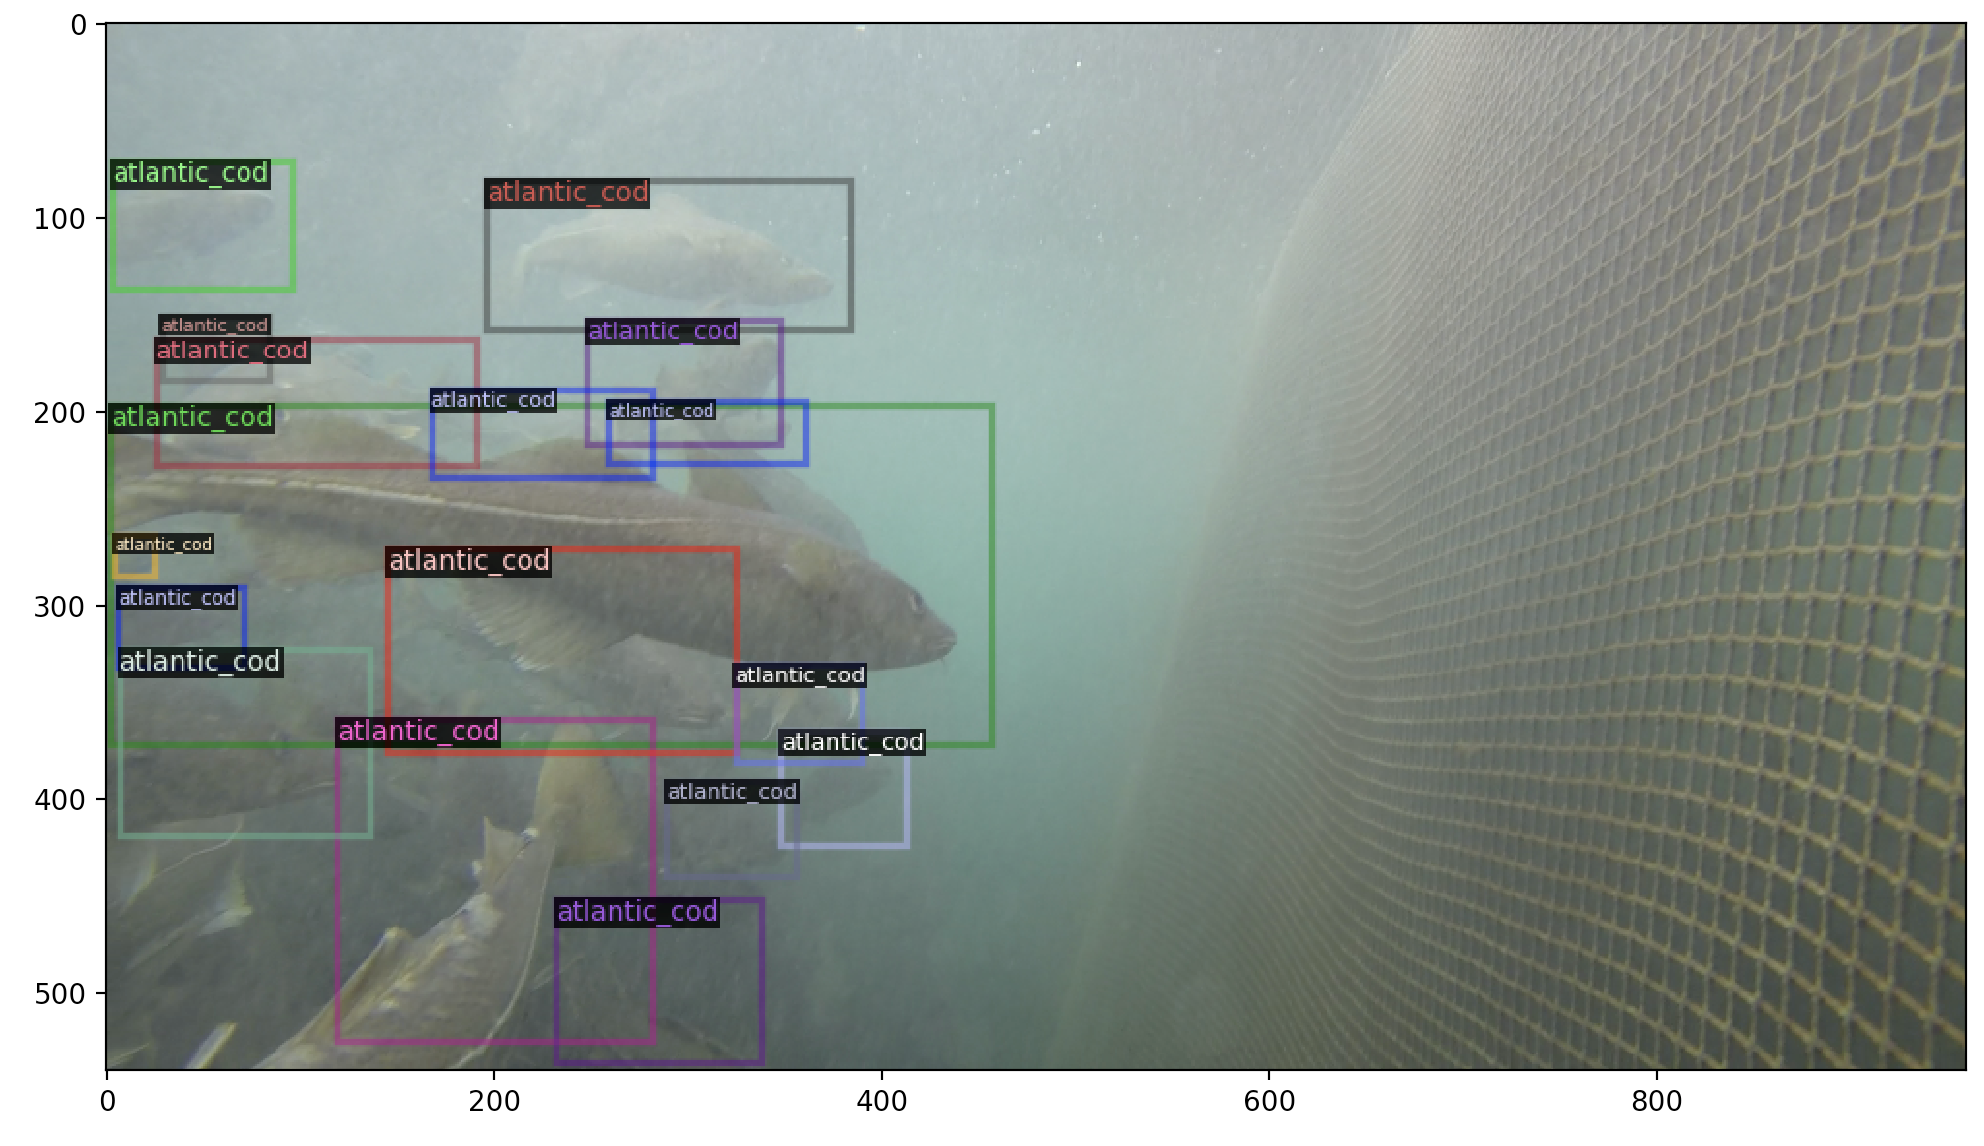
\includegraphics[scale=0.35]{figures/retinanet_cod}
\caption{\small \sl Figuren viser objektdeteksjon av torsk i lagringsmerd med RetinaNet. \label{fig:retinenet_inference}} 
\end{center} 
\end{figure} 

Ettersom OpenCV kunne ikke laste inn en PyTorch modell da denne oppgaven ble skrevet, så ble inferens gjort med Python, og det ble ikke gjort et forsøk på å gjøre inference i sanntid på en videostrøm med RetinaNet. Se resultater i figur \ref{fig:retinenet_inference} og \ref{fig:inference}.

Koden for inferens er under.

\begin{lstlisting}[language=Python, caption=Inferens RetinaNet i inference.py]
def video_read_write(video_path):
    """
    Read video frames one-by-one, flip it, and write in the other video.
    video_path (str): path/to/video
    """
    video = cv2.VideoCapture(video_path)
    
    # Check if camera opened successfully
    if not video.isOpened(): 
        print("Error opening video file")
        return
    
    # create video writer
    width = int(video.get(cv2.CAP_PROP_FRAME_WIDTH))
    height = int(video.get(cv2.CAP_PROP_FRAME_HEIGHT))
    frames_per_second = video.get(cv2.CAP_PROP_FPS)
    num_frames = int(video.get(cv2.CAP_PROP_FRAME_COUNT))
    
    isStreamOpen = False
    while video.isOpened():
        ret, frame = video.read()
        
        if ret:
            outputs = predictor(frame)

            #print(outputs)
            v = Visualizer(frame[:, :, ::-1],
                           metadata=test_metadata, 
                           scale=0.8
            )

            instances = outputs["instances"].to("cpu")

            v = v.draw_instance_predictions(instances)

            plt.imsave('outputs/frame_intermediate.png', v.get_image())

            if isStreamOpen == False:
                img = cv2.imread('outputs/frame_intermediate.png')
                height, width, layers = img.shape
                size = (width,height)
                out = cv2.VideoWriter('out.avi',cv2.VideoWriter_fourcc(*'DIVX'),
                		      frames_per_second, size)
                isStreamOpen = True

            img = cv2.imread('outputs/frame_intermediate.png')

            cv2.putText(img, 'num instances: ' + str(len(instances)), (5,100),
            		cv2.FONT_HERSHEY_SIMPLEX, 3, (0, 255, 0), 2, cv2.LINE_AA)
            out.write(img)

            print ('num instances: ' + str(len(instances)))
        else:
            break
    
    out.release()
    video.release()
    
    return

cfg.DATASETS.TEST = (test_data_name,)

# create a predictor instance with the configuration (it has our fine-tuned model)
# this predictor does prdiction on a single image
predictor = DefaultPredictor(cfg)

# create directory for evaluation
eval_dir = os.path.join(cfg.OUTPUT_DIR, 'coco_eval')
os.makedirs(eval_dir, exist_ok=True)

# create evaluator instance with coco evaluator
evaluator = COCOEvaluator(dataset_name=test_data_name,
                          cfg=cfg,
                          distributed=False,
                          output_dir=eval_dir)

# create validation data loader
val_loader = build_detection_test_loader(cfg, test_data_name)

# start validation 
inference_on_dataset(trainer.model, val_loader, evaluator)

# Run inference on video
video_read_write('in.mp4')
\end{lstlisting}

\subsubsection{OpenCV program} \label{part:opencv}

OpenCV (Open Source Computer Vision Library) er en åpenkildekode maskinsyn og maskinlæring programvarebibliotek. OpenCV ble laget for å levere en kjent infrastruktur for maskinsynprogrammer, OpenCV teamet ønsker å gjøre maskinsensorikk mer utbredt i kommersielle produkter. OpenCV er et produkt gitt ut under BSD-lisensen, det gjør biblioteket tilgjengelig for bedrifter som ønsker å anvende kildekoden. \cite{OpenCV Team 2020}

OpenCV har C++, Python, Java og MATLAB grensesnitt og støtter Windows, Linux, Android og macOS. OpenCV Teamet forsøker først og fremst å levere sanntids maskinsyn for dataprogrammer og drar nytte av prosessorteknologi slik som MMX og SSE instruksjoner når de er tilgjengelige. CUDA og OpenCL støtte var under utvikling, men var enda ikke tilgjengelig da denne oppgaven ble skrevet. Det hadde gjort dataprogrammet mye raskere, den ville dratt nytte av GPU-en og ikke bare CPU-en på maskinen. OpenCV er skrevet i C++ og virker uten konflikter med STL datastrukturer. \cite{OpenCV Team 2020}

Det ble skrevet et C++ program som bruker OpenCV til sanntids fiskedeteksjon med YOLOv4 modellen. OpenCV hadde fortsatt dårlig støtte av ONIX formatet, caffe2 formatet, og PyTorch da denne oppgaven ble skrevet. OpenCV 3.4 ble anvendt, da den fikk nylig støtte for YOLOv4. \cite{Batanina 2020}

\begin{figure}
\begin{center} 
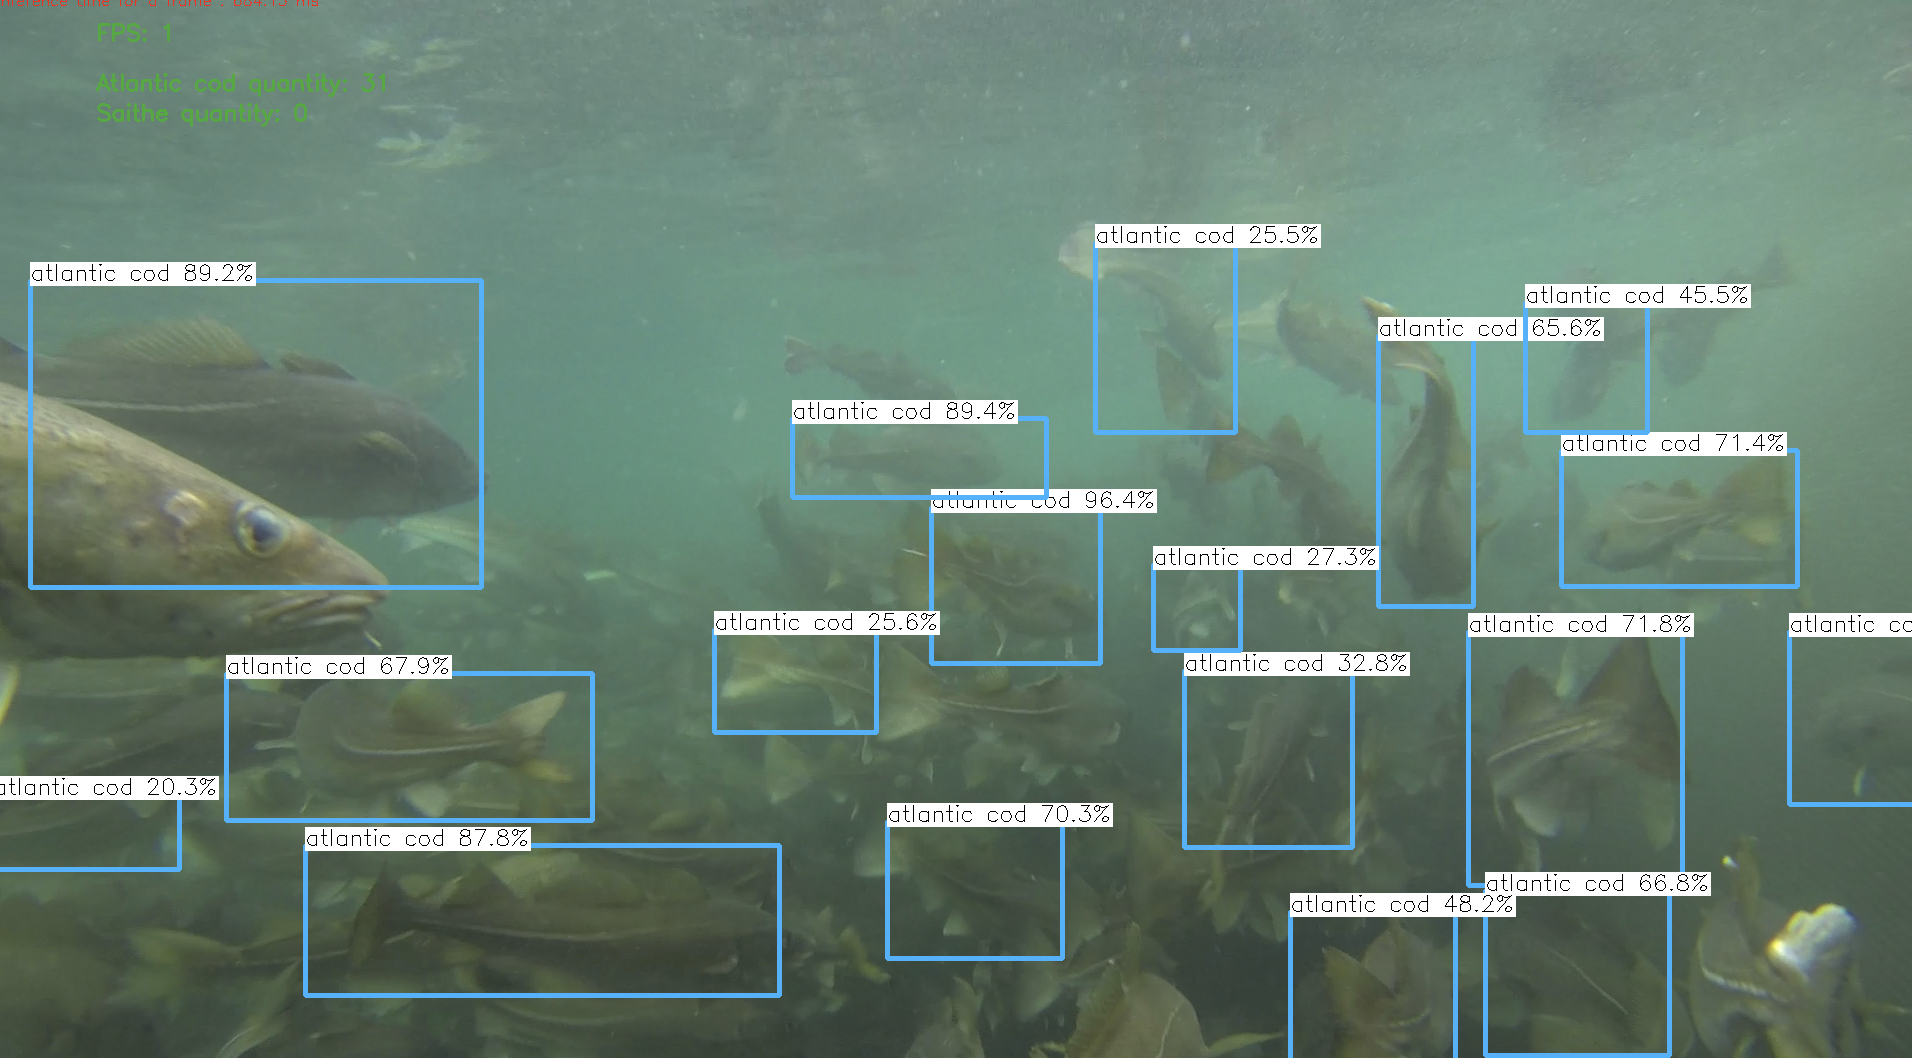
\includegraphics[scale=0.35]{figures/inference_yolo}
\caption{\small \sl Figuren viser inference med YOLOv4. Rundt fiskene så lager YOLOv4 bounding boxes der den tror det finnes fisk, og gir den en label basert på det den tror at det er. Her får alle fiskene labelen ``atlantic cod'', dette er fra en lagringsmerd med torsk. Ved siden av navnet av klassen så står det hvor sikker nettverket er på at den har funnet en torsk, presisjonen av inferensen. I grønn tekst, øverst til venstre, står det at algoritmen kan telle 31 torsk i bildet, og 0 sei. \label{fig:yolo_inference}} 
\end{center} 
\end{figure} 

Inferens med YOLOv4 ble gjort i OpenCV programmet. Programmet heter OBJECT\_DETECTOR, den laster inn en YOLOv4 konfigurasjon, en modell, og en videostrøm. Videostrømmen kan komme fra et kamera koblet til maskinen eller en fil på filsystemet. Programmet analyserer videostrømmen og logger mengden torsk og sei som blir observert. Se figur \ref{fig:yolo_inference}.

Når en lager et C++ program så må en kompilator og build-system bli valgt. For Windows så ble msvc++, som er en del av Visual Studio Community 2019, valgt. På macOS så ble clang brukt. Build-systemet cmake ble valgt. Alle disse verktøyene er tilgjengelig gratis, msvc++ er det eneste verktøyet som ikke er et åpen kildekodeprosjekt i tillegg til å være gratis. CMakeLists.txt beskriver C++ programmet. CMakelists.txt er en konfigurasjonsfil for cmake build-systemet, et av build systemene som kan brukes til å holde styr på C++ programmer. Det er nyttig å ha et IDE, en Intergrated Development Environment, når man programmerer i C++. QtCreator open source er et velutviklet IDE som kan laste inn cmake prosjekter.

OpenCV-prosjektet bruker også cmake, og er også skrevet i C++. Her installeres OpenCV fra kommandolinjen på et unix system.

\begin{verbatim}
mkdir opencv-3.4
cd opencv-3.4
git clone https://github.com/opencv/opencv
git clone https://github.com/opencv/opencv_contrib
cd opencv_contrib
git checkout 3.4
cd modules
dir=$(pwd)
cd ../../opencv
git checkout 3.4
mkdir build
cd build
cmake OPENCV_EXTRA_MODULES_PATH=$dir ..
make
make install
\end{verbatim}

\begin{figure}
\begin{center} 
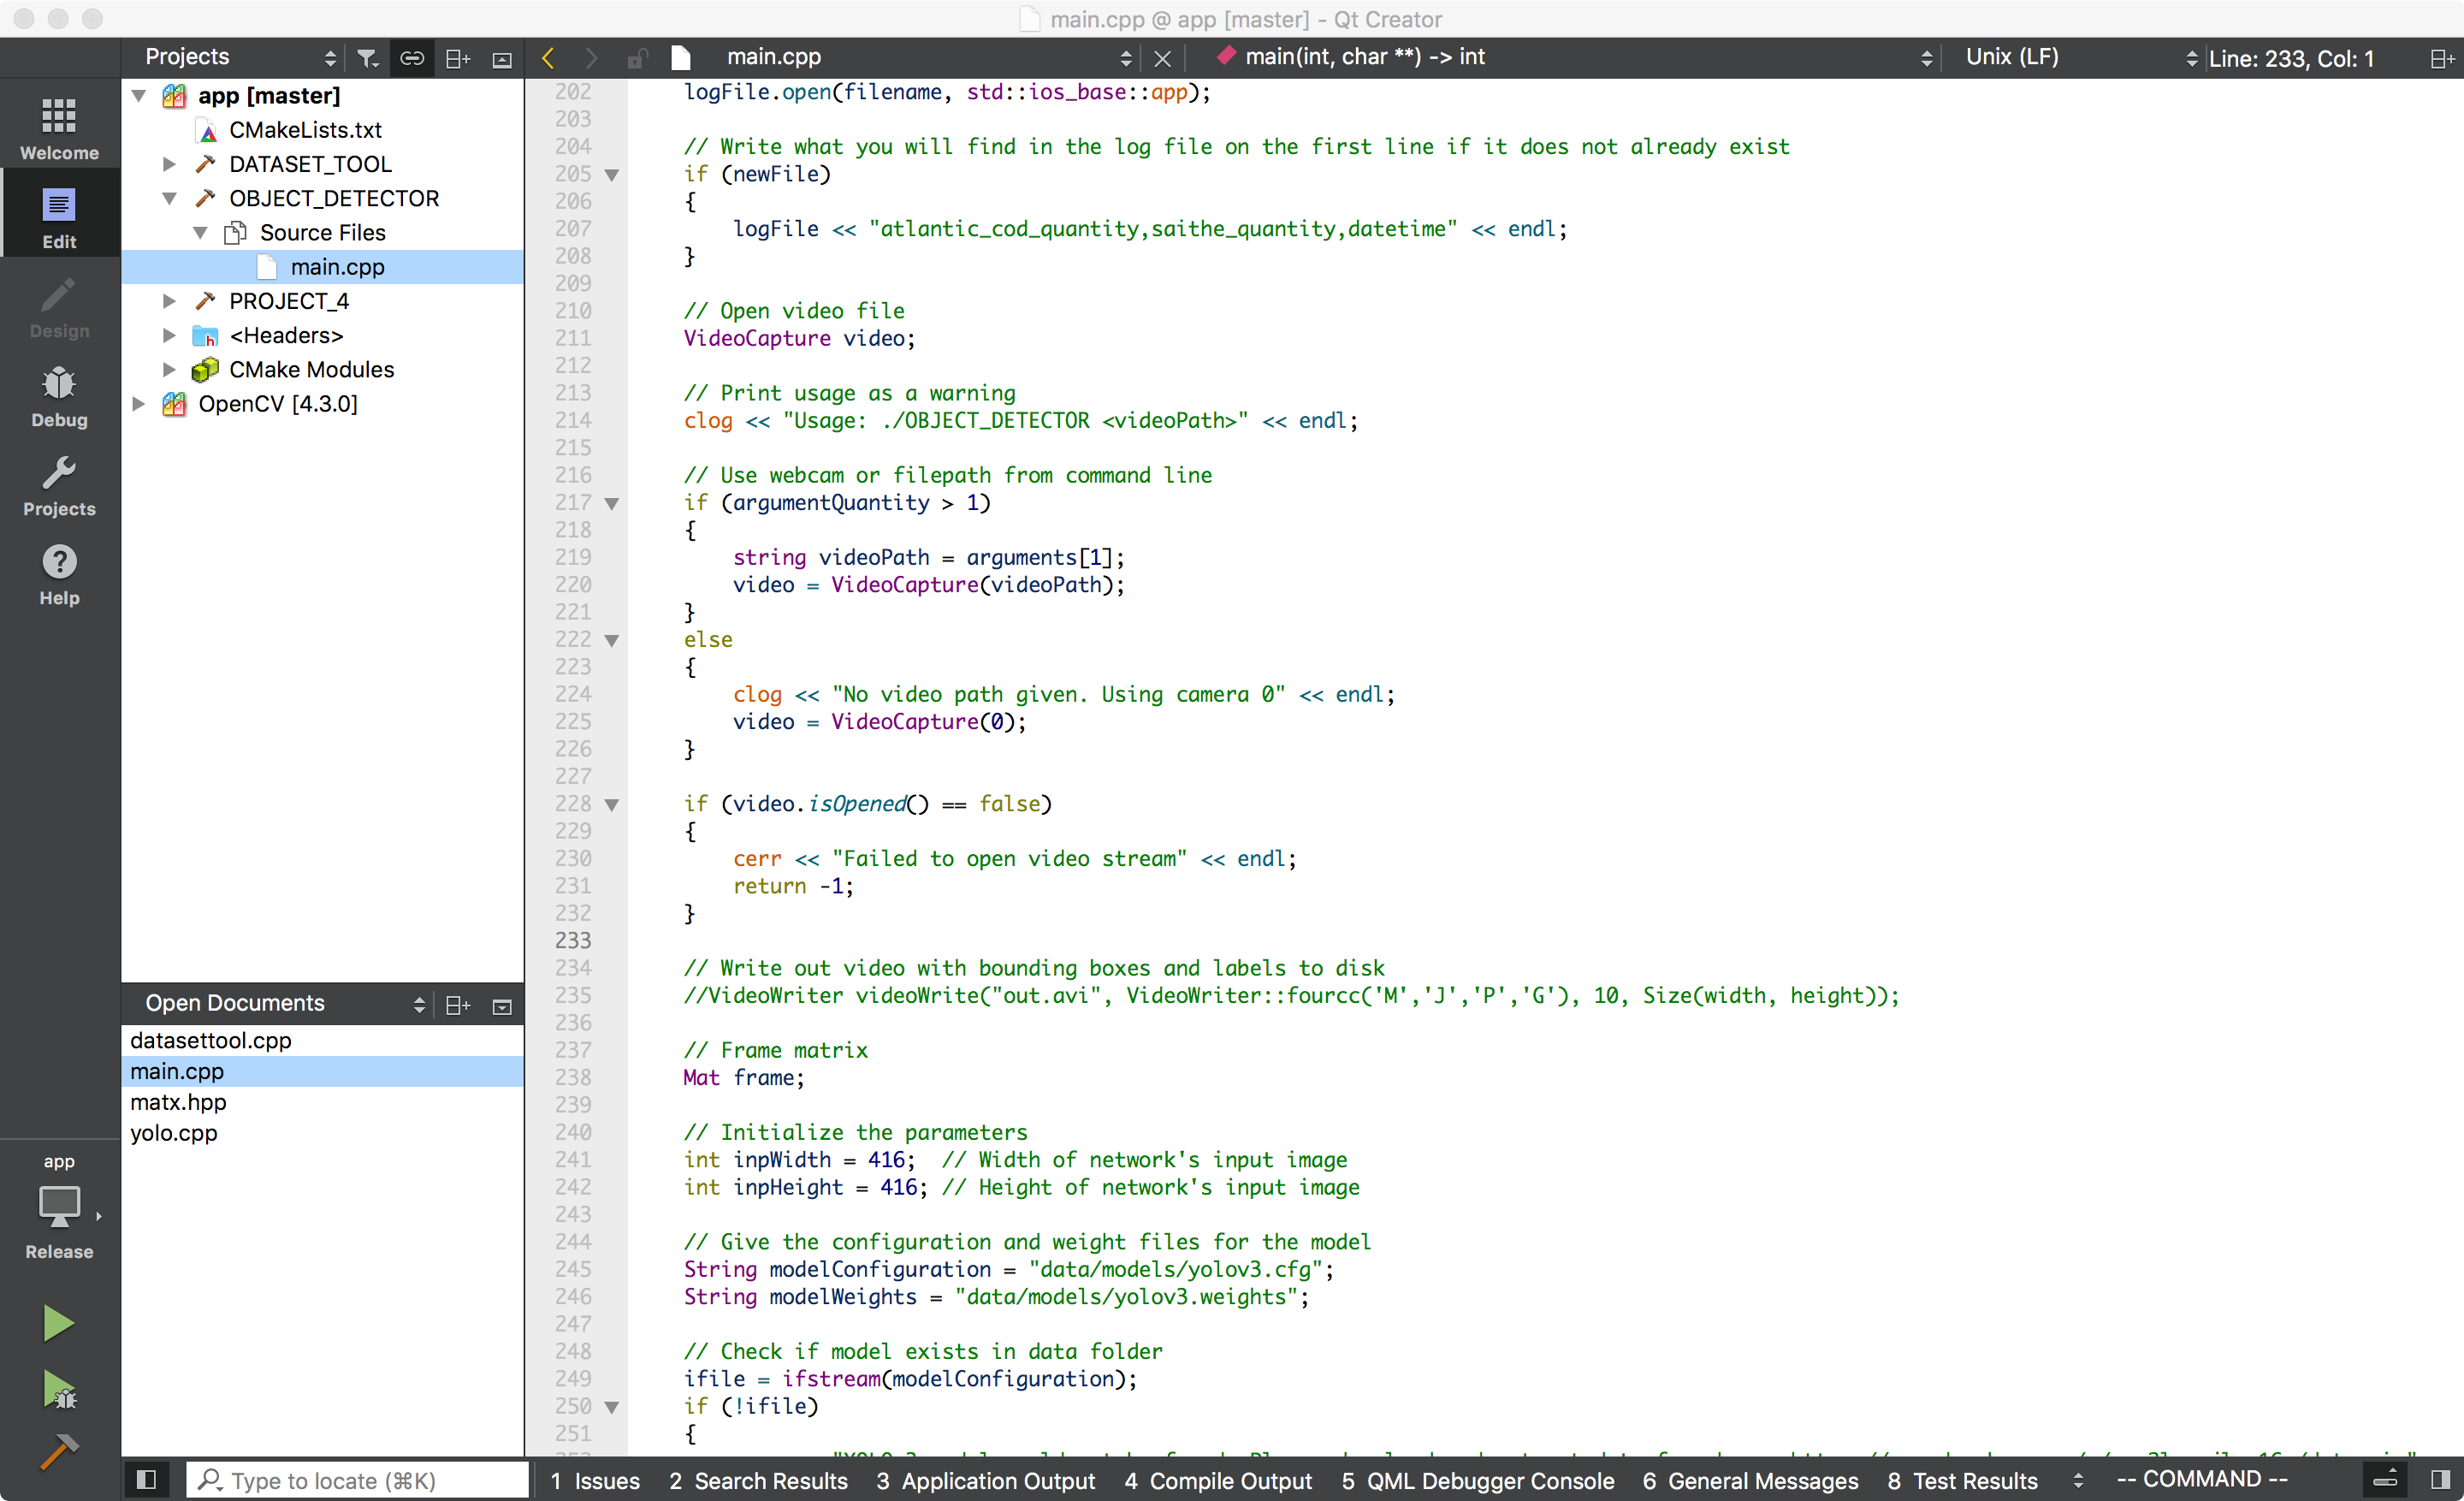
\includegraphics[scale=0.2]{figures/qtcreator}
\caption{\small \sl QtCreator. \label{fig:qtcreator}} 
\end{center} 
\end{figure} 

Det er også mulig å kompilere OpenCV med hjelp fra QtCreator. QtCreator open source ble lastet ned fra \url{https://www.qt.io/download}. CMakeLists.txt i opencv-3.4/opencv ble åpnet i QtCreator. OPENCV\_EXTRA\_MODULES\_PATH ble satt til opencv\_contrib/modules på filsystemet. Dette kan gjøres fra Projects modusen i QtCreator. Se sidepanelet i figur \ref{fig:qtcreator}.

Anaconda individual med python 2 ble brukt. Det ble laget en cmake CMakeLists.txt fil for prosjektet. Denne burde muligens endres om andre vil kompilere prosjektet, merk at anaconda ble installert til hjemmemappen til brukeren. Prosjektet består av to programmer. OBJECT\_DETECTOR gjør fiskedeteksjon. Se figur \ref{fig:yolo_inference}. DATASET\_TOOL ble brukt til å lage label data ut av videoer. Se figur \ref{fig:dataset_tool}.

\begin{lstlisting}[language=, caption=CMakeLists.txt]
cmake_minimum_required(VERSION 2.8.12)

PROJECT(app)
SET(CMAKE_CXX_STANDARD 14)

SET(Python2_ROOT_DIR ${PYTHONHOME})

find_package(Python2 COMPONENTS Development NumPy)

SET(OpenCV_DIR C:/opencv-3.4/opencv/build)

if( UNIX )
    include_directories(~/anaconda2/include/python2.7 ~/anaconda2/lib/python2.7/site-packages/numpy/core/include/ ~/anaconda2/include)
else()
    include_directories(${PYTHON_INCLUDE_DIRS} ~/Anaconda2/Lib/site-packages/numpy/core/include)
endif()

if(MSVC)
SET(CMAKE_CXX_FLAGS_RELEASE "${CMAKE_CXX_FLAGS_RELEASE} /MT")
endif()

find_package( OpenCV REQUIRED )

set(OpenCV_STATIC ON) # Easier to share binaries

include_directories( ${OpenCV_INCLUDE_DIRS} )

# If the package has been found, several variables will
# be set, you can find the full list with descriptions
# in the OpenCVConfig.cmake file.
# Print some message showing some of them
message(STATUS "OpenCV library status:")
message(STATUS "    config: ${OpenCV_DIR}")
message(STATUS "    version: ${OpenCV_VERSION}")
message(STATUS "    libraries: ${OpenCV_LIBS}")
message(STATUS "    include path: ${OpenCV_INCLUDE_DIRS}")

add_executable(OBJECT_DETECTOR main.cpp)
target_include_directories(OBJECT_DETECTOR PRIVATE ${PYTHON2_INCLUDE_DIRS} ${PYTHON2_NUMPY_INCLUDE_DIRS})
target_link_libraries(OBJECT_DETECTOR PRIVATE ${OpenCV_LIBS} Python2::Python ) # libs # "${TORCH_LIBRARIES}"

add_executable(DATASET_TOOL datasettool.cpp)
target_include_directories(DATASET_TOOL PRIVATE ${PYTHON2_INCLUDE_DIRS} ${PYTHON2_NUMPY_INCLUDE_DIRS})
target_link_libraries(DATASET_TOOL PRIVATE ${OpenCV_LIBS} Python2::Python ) # libs # "${TORCH_LIBRARIES}"
\end{lstlisting}

main.cpp er kildekoden til OBJECT\_DETECTOR. Først lastes bibliotekene inn.

\begin{lstlisting}[language=C++, caption=main.cpp]
#include <opencv2/opencv.hpp>
#include <opencv2/dnn.hpp>
//#include <opencv2/tracking.hpp>
#include <fstream>
//#include "matplotlibcpp.h"
#include <chrono>
#include <ctime>

using namespace std;
//using namespace matplotlibcpp;
using namespace cv::dnn;
using namespace cv;

// globals
float objectnessThreshold; // Objectness threshold
float confThreshold; // Confidence threshold
float nmsThreshold;  // Non-maximum suppression threshold
int inpWidth;  // Width of network's input image
int inpHeight; // Height of network's input image
vector<string> classes;

vector<Rect2d> bboxes;
int codQuantity, saitheQuantity;

string objectLabel;

const char *WINDOW_TITLE = "Press ESC to quit";
\end{lstlisting}

getOutputsNames henter ut label navn fra det ytterste laget i modellen. Se figur \ref{fig:deep}.

\begin{lstlisting}[language=C++, caption=main.cpp]
// Get the names of the output layers
auto getOutputsNames(const Net& net)
{
    static vector<String> names;
    if (names.empty())
    {
        // Get the indices of the output layers, i.e. the layers with unconnected outputs
        vector<int> outLayers = net.getUnconnectedOutLayers();

        // Get the names of all the layers in the network
        vector<String> layersNames = net.getLayerNames();

        // Get the names of the output layers in names
        names.resize(outLayers.size());
        for (size_t i = 0; i < outLayers.size(); ++i)
            names[i] = layersNames[outLayers[i] - 1];
    }
    return names;
}
\end{lstlisting}

drawPred lager en bounding box rundt objektene som detekteres av modellen.

\begin{lstlisting}[language=C++, caption=main.cpp]
// Draw the predicted bounding box
void drawPred(int classId, float conf, int left, int top, int right, int bottom, Mat& frame)
{
    // Draw a rectangle displaying the bounding box
    rectangle(frame, Point(left, top), Point(right, bottom), Scalar(255, 178, 50), 3);

    // Get the label for the class name and its confidence
    string label = format("%.1f", conf * 100);
    if (!classes.empty())
    {
        CV_Assert(classId < (int)classes.size());
        label = classes[classId] + " " + label + "\%";
    }

    // Display the label at the top of the bounding box
    int baseLine;
    Size labelSize = getTextSize(label, FONT_HERSHEY_SIMPLEX, 0.5, 1, &baseLine);
    top = max(top, labelSize.height);
    rectangle(frame, Point(left, top - round(1.5*labelSize.height)), Point(left + round(1.5*labelSize.width), top + baseLine), Scalar(255, 255, 255), FILLED);
    putText(frame, label, Point(left, top), FONT_HERSHEY_SIMPLEX, 0.75, Scalar(0,0,0),1);

    objectLabel = label;
}
\end{lstlisting}

postprocess henter alle instanser av fiskene i et bilde som er over en non-maxima suppression confidence boundary. Deretter sjekker den om objektet er en torsk eller sei, og teller mengden torsk og sei i bildet.

\begin{lstlisting}[language=C++, caption=main.cpp]
// Remove the bounding boxes with low confidence using non-maxima suppression
void postprocess(Mat& frame, const vector<Mat>& outs)
{
    vector<int> classIds;
    vector<float> confidences;
    vector<Rect> boxes;

    codQuantity = 0;
    saitheQuantity = 0;

    for (size_t i = 0; i < outs.size(); ++i)
    {
        // Scan through all the bounding boxes output from the network and keep only the
        // ones with high confidence scores. Assign the box's class label as the class
        // with the highest score for the box.
        float* data = (float*)outs[i].data;
        for (int j = 0; j < outs[i].rows; ++j, data += outs[i].cols)
        {
            Mat scores = outs[i].row(j).colRange(5, outs[i].cols);
            Point classIdPoint;
            double confidence;
            // Get the value and location of the maximum score
            minMaxLoc(scores, 0, &confidence, 0, &classIdPoint);

            if (confidence > confThreshold)
            {
                if (classes[classIdPoint.x] == "atlantic cod") {
                    codQuantity++;
                }
                else if (classes[classIdPoint.x] == "saithe")
                {
                    saitheQuantity++;
                }

                int centerX = (int)(data[0] * frame.cols);
                int centerY = (int)(data[1] * frame.rows);
                int width = (int)(data[2] * frame.cols);
                int height = (int)(data[3] * frame.rows);
                int left = centerX - width / 2;
                int top = centerY - height / 2;

                classIds.push_back(classIdPoint.x);
                confidences.push_back((float)confidence);
                boxes.push_back(Rect(left, top, width, height));

                /*if (isTracking == false)
                {
                    Rect2d bbox(centerX - (width / 2), centerY - (height / 2), width, height); // KCF works best with a tight crop
                    bboxes.push_back(bbox);

                    Ptr<Tracker> newTracker = createTrackerByName(trackerTypes[2]); // Use KCF
                    newTracker->init(frame, Rect2d(bboxes[i]));

                    trackers.push_back(newTracker);
                }*/
            }
        }
    }

    // Perform non maximum suppression to eliminate redundant overlapping boxes with
    // lower confidences
    vector<int> indices;
    NMSBoxes(boxes, confidences, confThreshold, nmsThreshold, indices);
    for (size_t i = 0; i < indices.size(); ++i)
    {
        int idx = indices[i];
        Rect box = boxes[idx];
        drawPred(classIds[idx], confidences[idx], box.x, box.y,
                 box.x + box.width, box.y + box.height, frame);
    }

    //isTracking = true;
}
\end{lstlisting}

main er programmets main-entry point. Det er her dataprogrammet starter. Den åpner en logg, log.csv, og så åpner den en videostrøm. Deretter laster den inn YOLOv4 modellen.

\begin{lstlisting}[language=C++, caption=main.cpp]
int main(int argumentQuantity, char *arguments[])
{
    // Configuration for log file
    string filename = "log.csv";
    bool newFile = true;

    // Check if log file exists
    ifstream ifile(filename);
    if (ifile)
    {
        newFile = false;
    }

    // Open log file
    ofstream logFile;
    logFile.open(filename, std::ios_base::app);

    // Write what you will find in the log file on the first line if it does not already exist
    if (newFile)
    {
        logFile << "atlantic_cod_quantity,saithe_quantity,datetime" << endl;
    }

    // Open video file
    VideoCapture video;

    // Print usage as a warning
    clog << "Usage: ./OBJECT_DETECTOR <videoPath>" << endl;

    // Use webcam or filepath from command line
    if (argumentQuantity > 1)
    {
        string videoPath = arguments[1];
        video = VideoCapture(videoPath);
    }
    else
    {
        clog << "No video path given. Using camera 0" << endl;
        video = VideoCapture(0);
    }

    if (video.isOpened() == false)
    {
        cerr << "Failed to open video stream" << endl;
        return -1;
    }

    // Write out video with bounding boxes and labels to disk
    //VideoWriter videoWrite("out.avi", VideoWriter::fourcc('M','J','P','G'), 10, Size(width, height));

    // Frame matrix
    Mat frame;

    // Initialize the parameters
    int inpWidth = 416;  // Width of network's input image
    int inpHeight = 416; // Height of network's input image

    // Give the configuration and weight files for the model
    String modelConfiguration = "data/models/yolov3.cfg";
    String modelWeights = "data/models/yolov3.weights";

    // Check if model exists in data folder
    ifile = ifstream(modelConfiguration);
    if (!ifile)
    {
        cerr << "YOLOv3 model could not be found. Please download and extract data from here: https://www.dropbox.com/s/aym2lmnzjlam16v/data.zip" << endl;
        return -1;
    }

    // Load the network
    Net net = readNetFromDarknet(modelConfiguration, modelWeights);

    // Load names of classes
    string classesFile = "data/models/obj.names";
    ifstream ifs(classesFile.c_str());
    string line;
    while (getline(ifs, line)) classes.push_back(line);

    // Configure user interface
    namedWindow(WINDOW_TITLE, WINDOW_AUTOSIZE);
\end{lstlisting}

Den neste kodesnutten er programmets main loop. Denne koden repeteres til videoen har gått tomt for bilder, eller at brukeren trykker på ESC på tastaturet. For hvert bilde i videostrømmen så lagres antall torsk og sei observert til log.csv, med mindre det er ingen torsk eller sei som blir oppdaget.

\begin{lstlisting}[language=C++, caption=main.cpp]
    // Main loop
    bool isAlive = true;
    const int ESCAPE_KEYCODE = 27;
    const int DELAY_MILLISECONDS = 1;

    int key;

    while(isAlive)
    {
        key = waitKey(DELAY_MILLISECONDS);

        if (key == ESCAPE_KEYCODE)
        {
            isAlive = false;
            break;
        }

        double timer = (double)getTickCount();

        video >> frame;

        if (frame.empty())
        {
            isAlive = false;
            break;
        }

        // Create a 4D blob from a frame.
        Mat blob;
        blobFromImage(frame, blob, 1/255.0, Size(inpWidth, inpHeight), Scalar(0,0,0), true, false);

        //Sets the input to the network
        net.setInput(blob);

        // Runs the forward pass to get output of the output layers
        vector<Mat> outs;
        net.forward(outs, getOutputsNames(net));

        // Remove the bounding boxes with low confidence
        postprocess(frame, outs);

        // Put efficiency information. The function getPerfProfile returns the overall time for inference(t) and the timings for each of the layers(in layersTimes)
        vector<double> layersTimes;
        double freq = getTickFrequency() / 1000;
        double t = net.getPerfProfile(layersTimes) / freq;
        string label = format("Inference time for a frame : %.2f ms", t);
        putText(frame, label, Point(0, 15), FONT_HERSHEY_SIMPLEX, 0.5, Scalar(0, 0, 255));

        float fps = getTickFrequency() / ((double)getTickCount() - timer);

        putText(frame, "FPS: " + std::to_string(int(fps)), Point(100,50), FONT_HERSHEY_SIMPLEX, 0.75, Scalar(50,170,50), 2);
        putText(frame, "Atlantic cod quantity: " + std::to_string(codQuantity), Point(100,100), FONT_HERSHEY_SIMPLEX, 0.75, Scalar(50,170,50), 2);
        putText(frame, "Saithe quantity: " + std::to_string(saitheQuantity), Point(100,130), FONT_HERSHEY_SIMPLEX, 0.75, Scalar(50,170,50), 2);

        //videoWrite.write(frame);
        imshow(WINDOW_TITLE, frame);

        // Get the time
        auto end = std::chrono::system_clock::now();
        std::time_t end_time = std::chrono::system_clock::to_time_t(end);

        // Remove the newline after time which is typically included from the C library call
        char *time = ctime(&end_time);
        if (time[strlen(time)-1] == '\n') time[strlen(time)-1] = '\0';

        // Log cod and saith quantities to csv file
        if (codQuantity > 0 || saitheQuantity > 0)
        {
            logFile << codQuantity << "," << saitheQuantity << ",\"" << time << "\"" << endl;
            cout << codQuantity << "," << saitheQuantity << ",\"" << time << "\"" << endl;
        }
    }

    logFile.close();

    video.release();
    //videoWrite.release();

    destroyAllWindows();

    return 0;
}
\end{lstlisting}

%\subsection{COCO Detection Evaluation} % For analyse kapittelet?

\subsection{Segmentering}

\begin{figure}[h!]
\begin{center} 
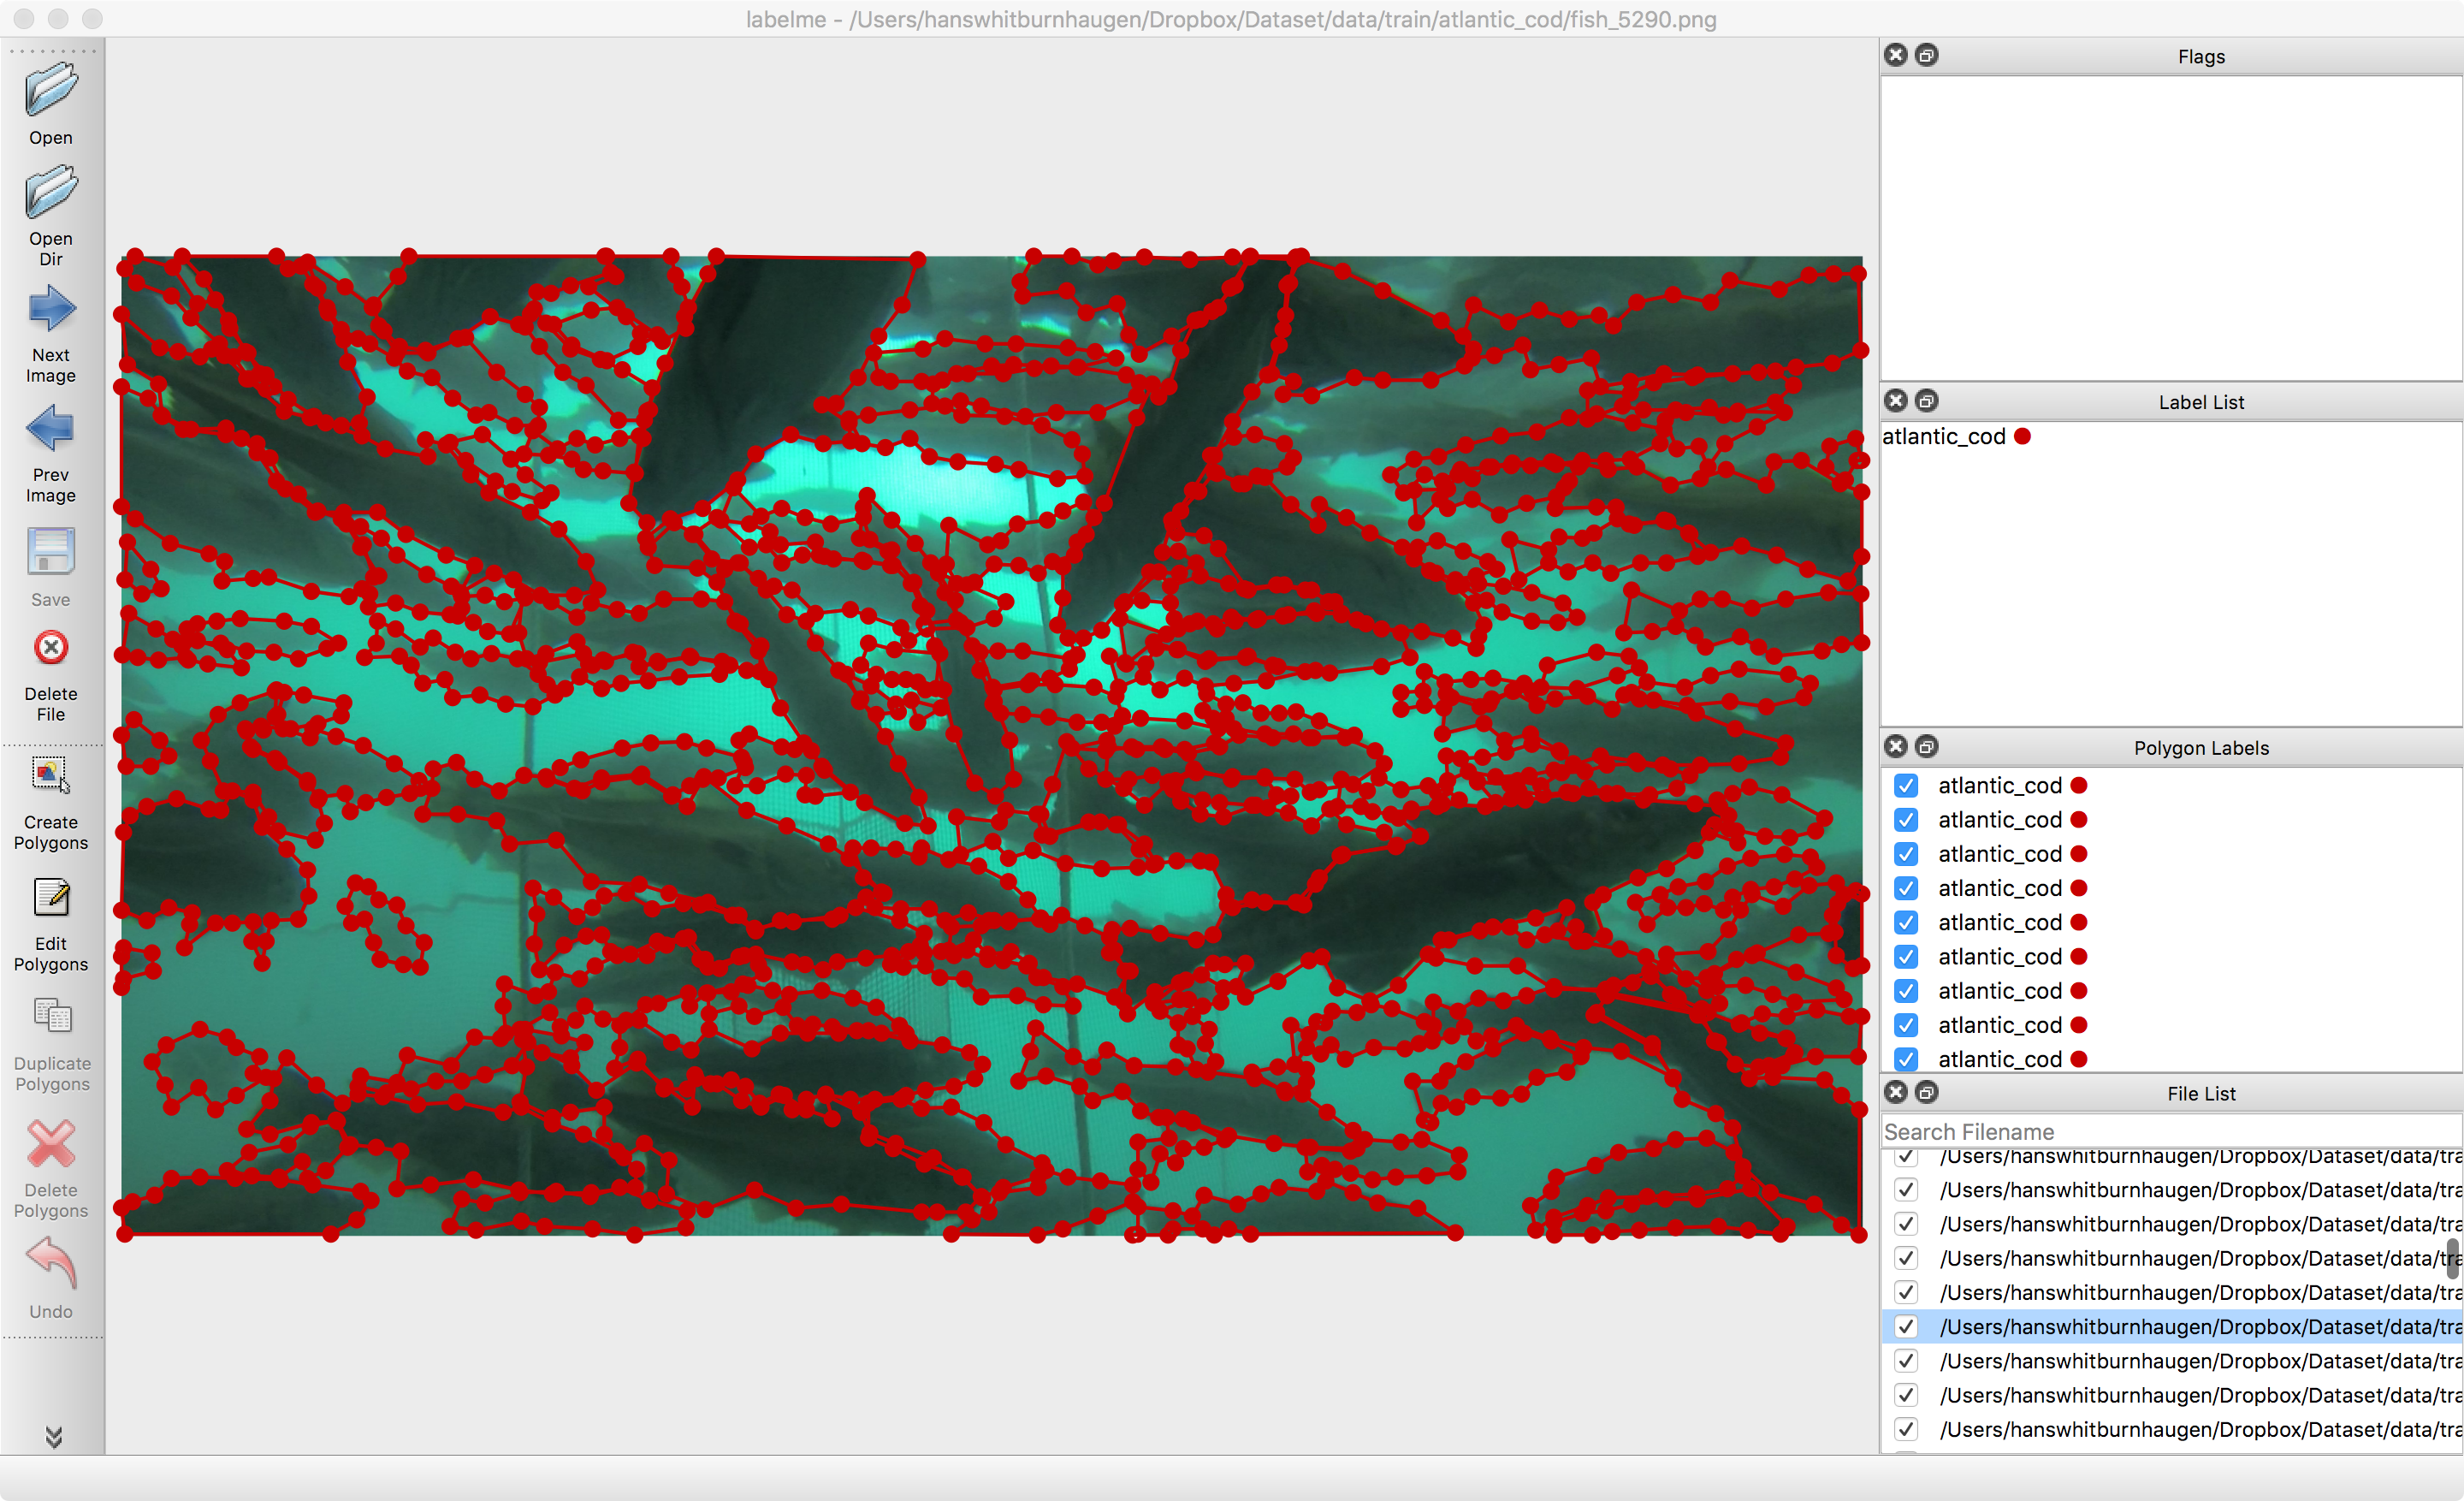
\includegraphics[scale=0.25]{figures/labelme}
\caption{\small \sl Figuren viser dataprogrammet labelme. \cite{Wada 2016} \label{fig:labelme}} 
\end{center} 
\end{figure} 

% Resultat 1/5 
%Å analysere gjør du ved å redegjøre, forklare og vurdere funnene dine. Analysedelen av oppgaven blir ofte kalt resultater, slik som i IMRoD-modellen.

%I kvantitative studier vil du kanskje i tillegg til å presentere funnene skriflig, bruke figurer og tabeller for å gi leseren en oversikt og innsikt i hva du har gjort.
%I empirisk baserte studier vil analysene handle om å beskrive og tolke. Mange vil ofte drøfte enkeltfunnene i dette kapitlet og ta for seg mer overordnede funn i drøftingskapitlet.
%Et lurt tips for å finne ut hvordan du kan skrive ditt analysekapittel, er å se hvordan det er gjort i andre oppgaver på tilsvarende nivå fra samme felt.

\section{Resultater}
\label{part:results}

Det ble trent opp to modeller, en RetinaNet-modell og en YOLOv4-modell. Se figur \ref{fig:inference} og \ref{fig:yolo_inference}. Dataen av torsk bestod av tre kanaler, og hadde størrelsen 1920 $\times$ 1080. Bildene av sei bestod av kun en kanal, og hadde størrelsen 640 $\times$ 480. Se figur \ref{fig:data}.

%A classification accuracy of 94.3 \% was achieved when classifying only the 16 fish species which we focussed on for this trial. All other evaluations include the other species class which contains a number of fish species which are non-relevant to the research goals, but can be encountered while underwater sampling. The re- sults obtained by the different model configurations are summa- rized in Table 2. The model based on ResNet (He et al., 2016) by cross-pooling activations from layer 4b15 and 4b20, with local region size of 3 and training of a linear SVM on top of the cross-pooled features, was able to achieve the highest classifica- tion accuracy of 89.0 \% if the other species class is included. A change to a local region size of 1 produces a slightly inferior result of 86.9 \% classification accuracy for all classes. In compari- son, the AlexNet and VGGNet model configurations produced significantly degraded results.

%Application of the linear SVM di- rectly to features from the Pool5 layer of the ResNet-152 model resulted in a classification accuracy of 71.49 \%, highlighting the improved performance produced by cross-layer pooling. We re- duced the dimensionality of the 3 local features in ResNet- 152b model from 9216 (3 3 1024) to 512 before cross-layer pooling using PCA. Dimensionality reduction can be useful in or- der to reduce the size of features from cross-layer pooling, allow- ing use of larger region sizes as well as more feature maps. Adapting a larger region size even with the use of PCA improved accuracy of the system due to availability of local context. 

%Further analysis of the accuracy of the four CNN models can be con- ducted using the precision and recall of the classifier. Recall and precision are a more informative way to judge the performance of a classifier, especially if the classes are skewed.


%The precision of a classifier is a measure of correctly classified images out of all the images predicted to belong to a specific class. Mathematically,

%In general, the precision and recall graphs confirm the classifi- cation accuracy levels shown in Table 2, with very few exceptions. In some cases, the ResNet-152 model with a 1 1 local region produces the best result, but these exceptions reflect the small dif- ference in the classification accuracy between the two sizes of lo- cal region. Precision is generally higher than recall, indicating that false negatives are more common than false positives. The precision graph shows high values for a number of individual species, indicating that the number of false positives is very low. The lesser precision in ...

\subsection{RetinaNet}

\begin{figure}[h!]
\begin{center} 
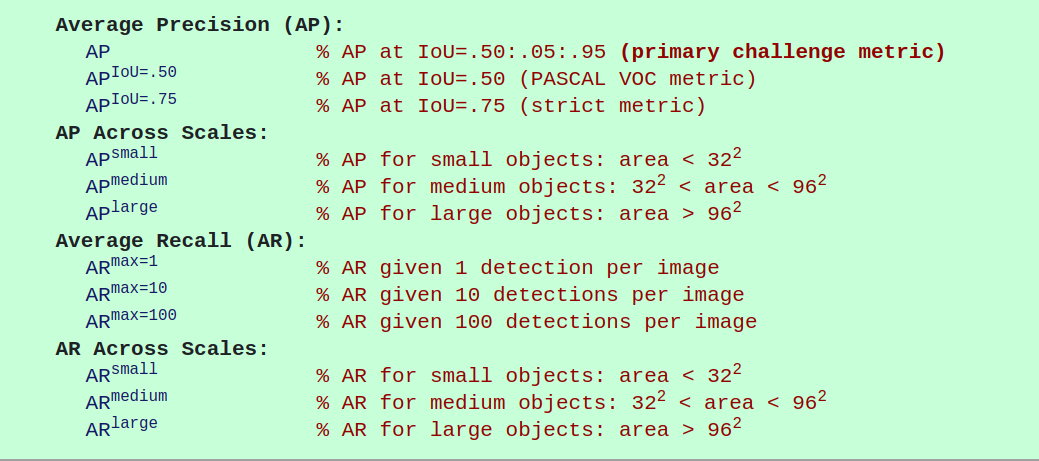
\includegraphics[scale=0.35]{figures/coco}
\caption{\small \sl Evalueringskortet til COCO. En modell som har blitt trent med vekter fra COCO kan evalueres etter dette kortet. \label{fig:coco}}
\end{center}
\end{figure}

AP står for «Average Precision», og AR står for «Average Recall». De er mål på hvor nøyaktig en deep learning-modell er. Se tabellene på side \pageref{tab:ap_retinanet}.

\begin{table}[]
\bigskip
\centering
\label{tab:ap_retinanet} 
\caption{AP (primary challenge metric) og Average Recall}
\begin{tabular}[t]{lccc}
\toprule
 Average Precision  (AP) @ [ IoU=0.50:0.95 & area=   all & maxDets=100 ] &= 0.285 \\
 Average Precision  (AP) @ [ IoU=0.50      & area=   all & maxDets=100 ] &= 0.663 \\
 Average Precision  (AP) @ [ IoU=0.75      & area=   all & maxDets=100 ] &= 0.200 \\
 Average Precision  (AP) @ [ IoU=0.50:0.95 & area= small & maxDets=100 ] &= 0.067 \\
 Average Precision  (AP) @ [ IoU=0.50:0.95 & area=medium & maxDets=100 ] &= 0.217 \\
 Average Precision  (AP) @ [ IoU=0.50:0.95 & area= large & maxDets=100 ] &= 0.402 \\
\midrule
 Average Recall     (AR) @ [ IoU=0.50:0.95 & area=   all & maxDets=  1 ] &= 0.038 \\
 Average Recall     (AR) @ [ IoU=0.50:0.95 & area=   all & maxDets= 10 ] &= 0.248 \\
 Average Recall     (AR) @ [ IoU=0.50:0.95 & area=   all & maxDets=100 ] &= 0.433 \\
 Average Recall     (AR) @ [ IoU=0.50:0.95 & area= small & maxDets=100 ] &= 0.139 \\
 Average Recall     (AR) @ [ IoU=0.50:0.95 & area=medium & maxDets=100 ] &= 0.352 \\
 Average Recall     (AR) @ [ IoU=0.50:0.95 & area= large & maxDets=100 ] &= 0.556 \\
 \bottomrule	
 \end{tabular}
\end{table}

\begin{table}[]
\bigskip
\centering
\caption{Evaluation results for bbox} 
\label{tab:bbox_retinanet} 
\begin{tabular}[t]{lccccc}
\toprule
   AP   &  AP50  &  AP75  &  APs  &  APm   &  APl    \\
 \midrule
 28.494 & 66.262 & 20.016 & 6.654 & 21.663 & 40.239 \\
 \bottomrule	
 \end{tabular}
\end{table}

\begin{table}[]
\bigskip
\centering
\label{tab:per-category_bbox_retinanet} 
\caption{Per-category bbox AP} 
\begin{tabular}[t]{lccc}
\toprule
 category     & AP     & category   & AP      \\
 \midrule
 atlantic\_cod & 23.077 & saithe     & 33.910 \\
 \bottomrule	
\end{tabular}
\end{table}

\subsubsection{COCO deteksjonsevaluering} 

Resultatene i tabell \ref{tab:ap_retinanet} kan sammenlignes med evalueringskortet i figur \ref{fig:coco}. Resultatene bør være bedre enn COCO-evalueringskortet. AP (primary challenge metric) bør være mer enn 0,5. RetinaNet-modellen har en AP lik 0,285. Se tabell \ref{tab:ap_retinanet}. AP for torsk var 23,1 \%, og 33,9 \% for sei. Se tabell \ref{tab:per-category_bbox_retinanet}.

%\begin{figure}[h!]
%\begin{center} 
%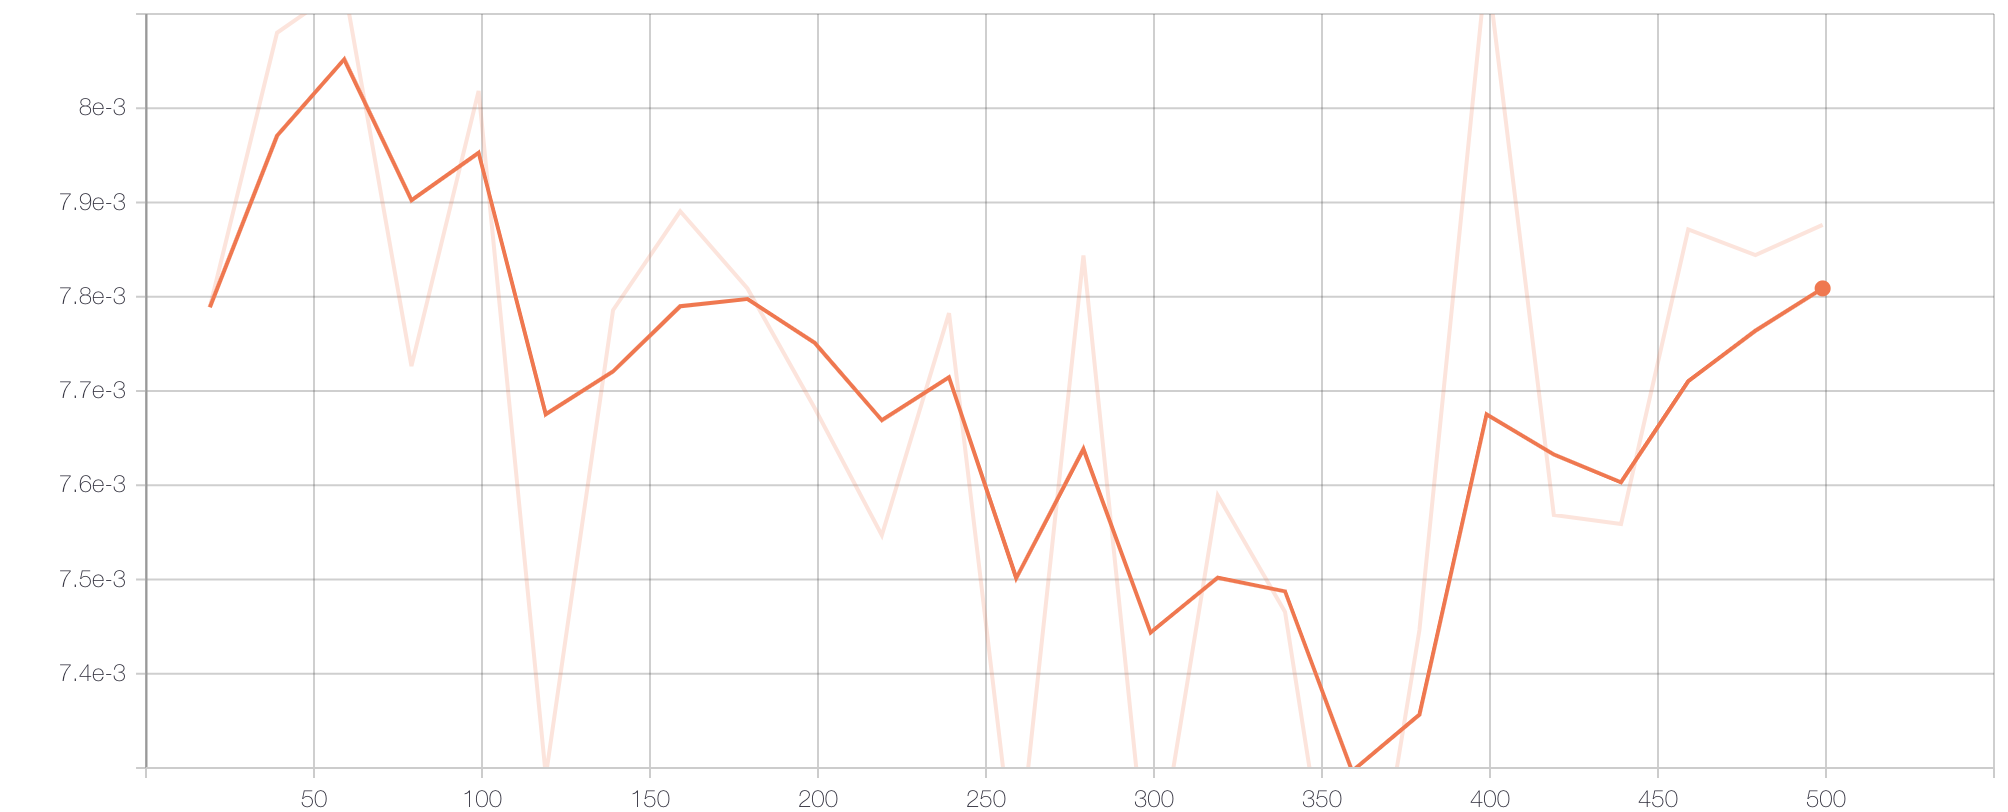
\includegraphics[scale=0.35]{figures/data_time_retinanet_1}
%\caption{\small \sl data time RetinaNet. \label{fig:data_time_retinanet}}
%\end{center}
%\end{figure}

%\begin{figure}[h!]
%\begin{center} 
%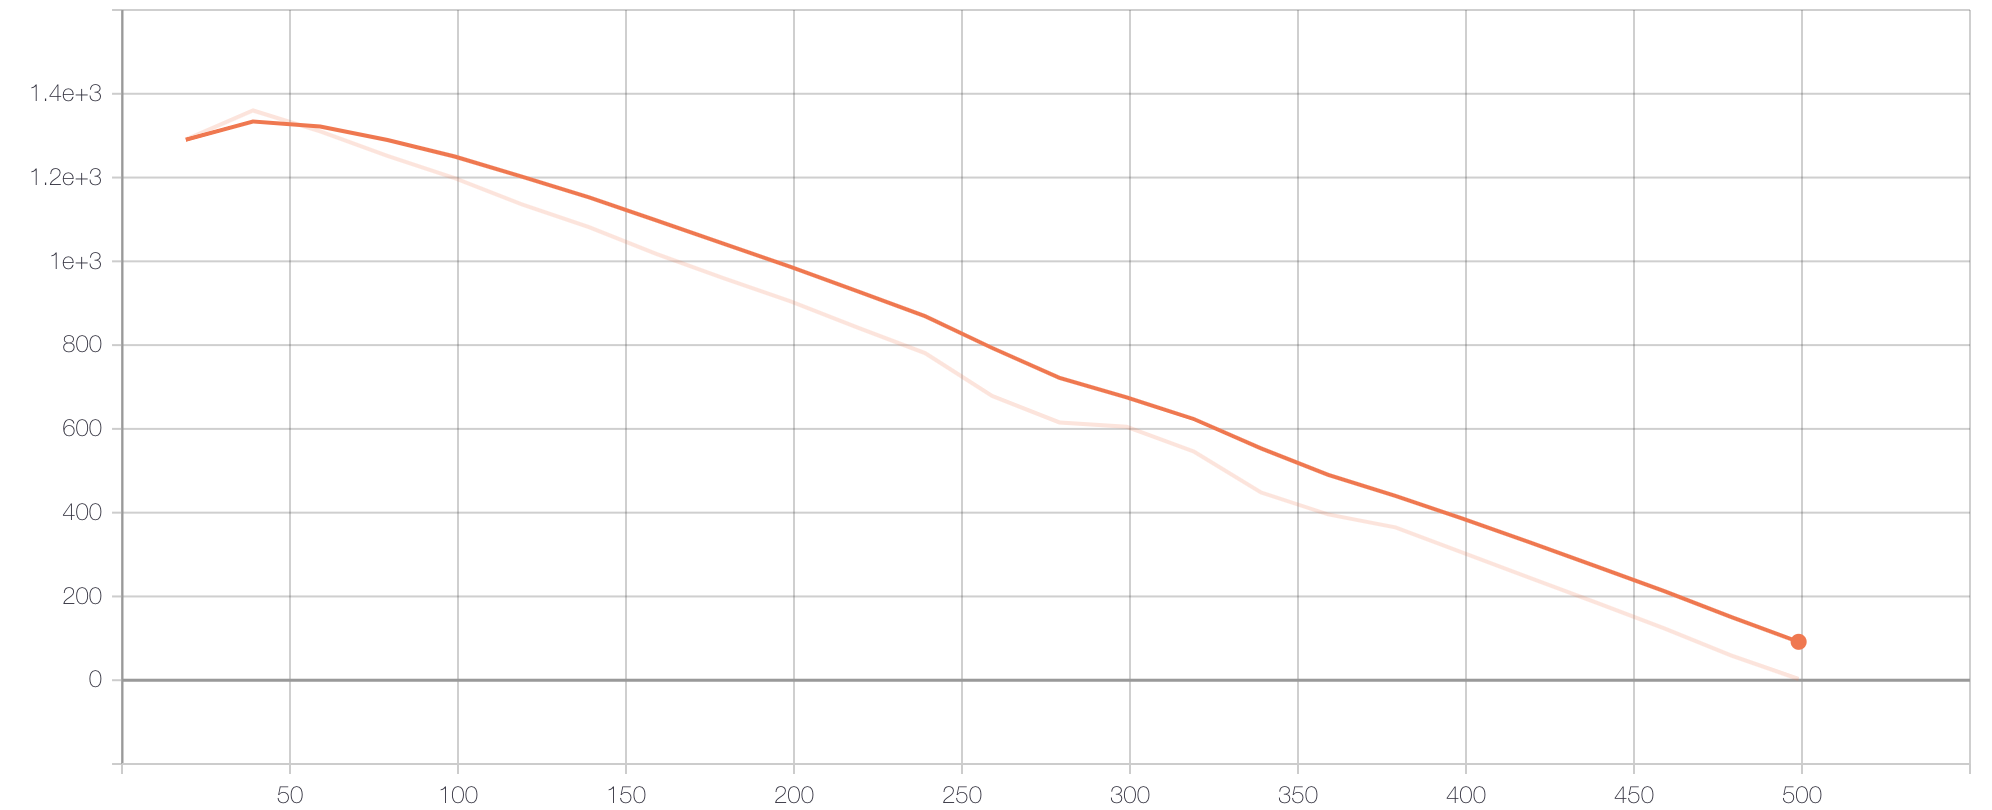
\includegraphics[scale=0.35]{figures/eta_seconds_retinanet_2}
%\caption{\small \sl eta seconds RetinaNet. \label{fig:eta_seconds_retinanet}}
%\end{center}
%\end{figure}

\subsubsection{TensorBoard resultater}

Alle grafene under er fra TensorBoard, et verktøy fra Google som er utviklet til å hjelpe dataforskere med å trene opp deep learning-modeller og dele resultatene til forsøkene deres. TensorBoard visualiserer maskinlæringseksperimenter og er egentlig laget for Google sin deep learning-rammeverk som heter Tensorflow, men PyTorch støtter også TensorBoard \cite{Oshri 2019}. Resultatene lastes opp med kommandoen \texttt{tensorboard dev upload --logdir logs --name 'TMAT3004' --description 'Bachelorprosjekt NTNU 2020'}.

I alle grafene fra TensorBoard, figur \ref{fig:loss_box_reg_retinanet}, \ref{fig:loss_cls_retinanet}, \ref{fig:lr_retinanet} og \ref{fig:total_loss_retinanet}, så er x-aksen tid i sekunder fra begynnelsen av forsøket, og y-aksen verdien til den spesifikke målingen. 

Modellene bør iterativt forbedres, og resultatene sammenlignes for hvert forsøk. Det er best å endre kun en parameter om gangen og se om modellen blir bedre. Dette er tidkrevende. TensorBoard gjør det lettere å sammenligne nye resultater med eldre resultater, grafene under viser to forsøk, hver figur har to grafer. Det nyeste forsøket er den mørkeste grafen.

Den første grafen nedenfor er «loss bounding box». Dette er et mål på hvor tett modellen satt bounding box-ene rundt objektene som fantes i bildene den gjorde inferens på.

\begin{figure}[H]
\begin{center} 
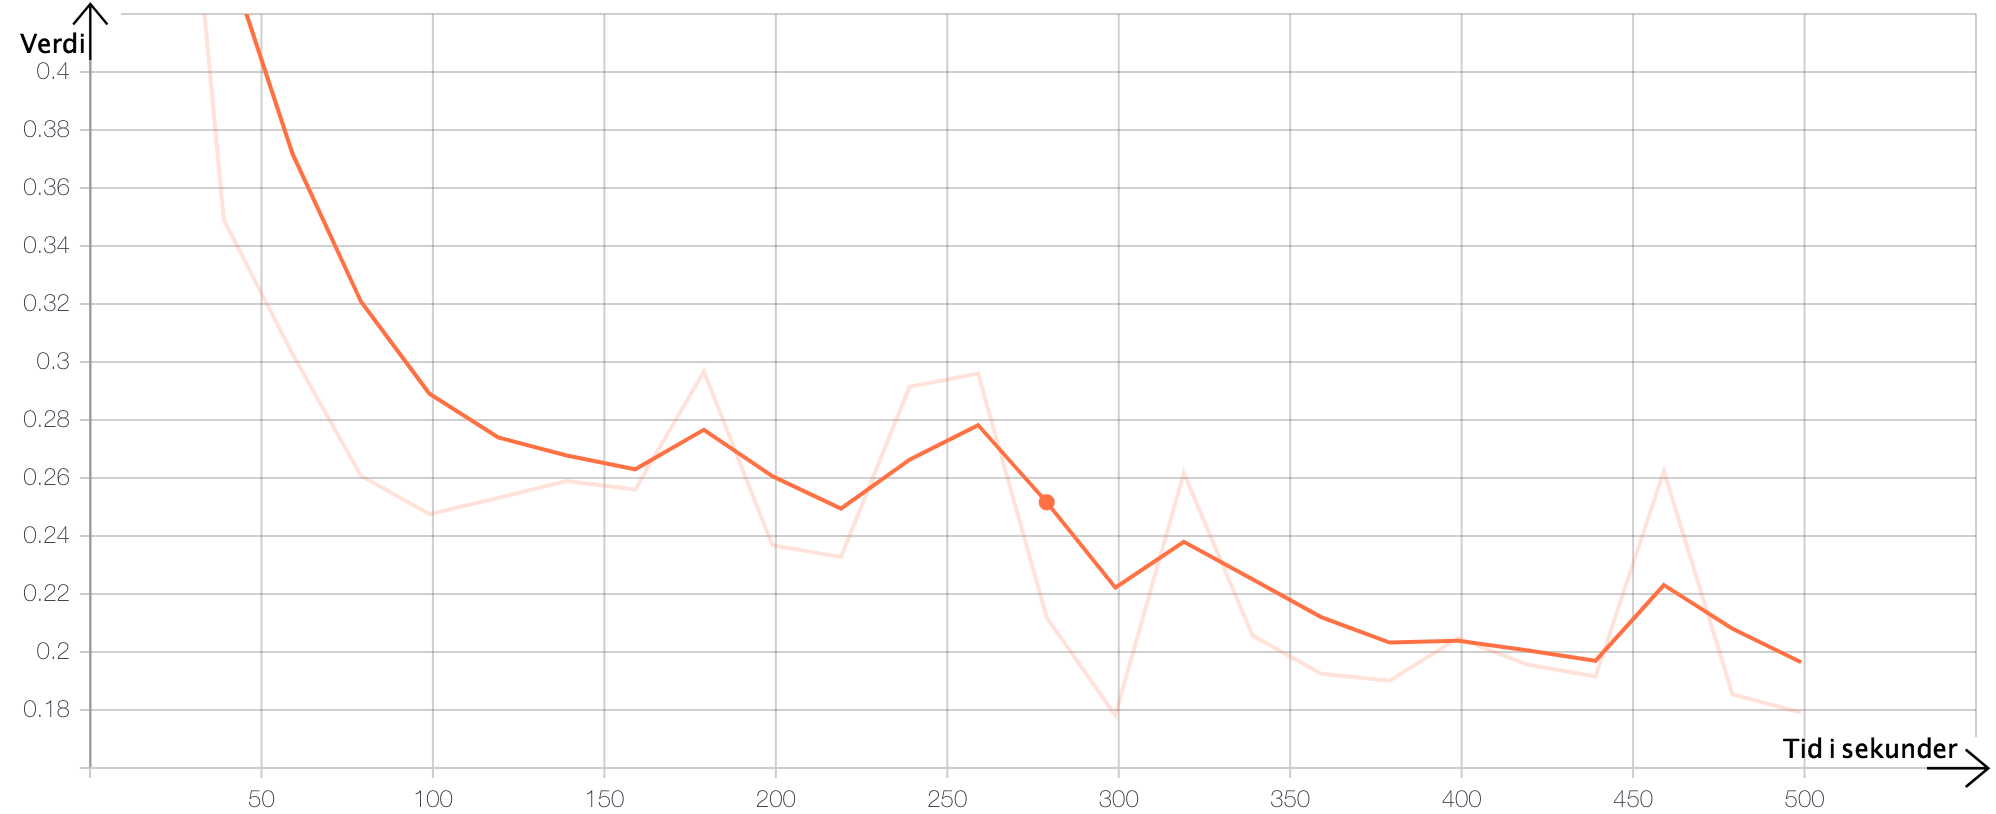
\includegraphics[scale=0.35]{figures/loss_box_reg_retinanet_3}
\caption{\small \sl «Loss bounding box» for RetinaNet. \label{fig:loss_box_reg_retinanet}}
\end{center}
\end{figure}

Neste graf viser «loss cls», eller «entropy loss». Entropy loss er et mål på hvor korrekt klassifiseringen av hver «bounding box» var. Hver «bounding box» kan inneholde en klasse, altså et objekt, eller være bakgrunn, og dermed være en boks som ikke inneholder en klasse.

\begin{figure}[H]
\begin{center} 
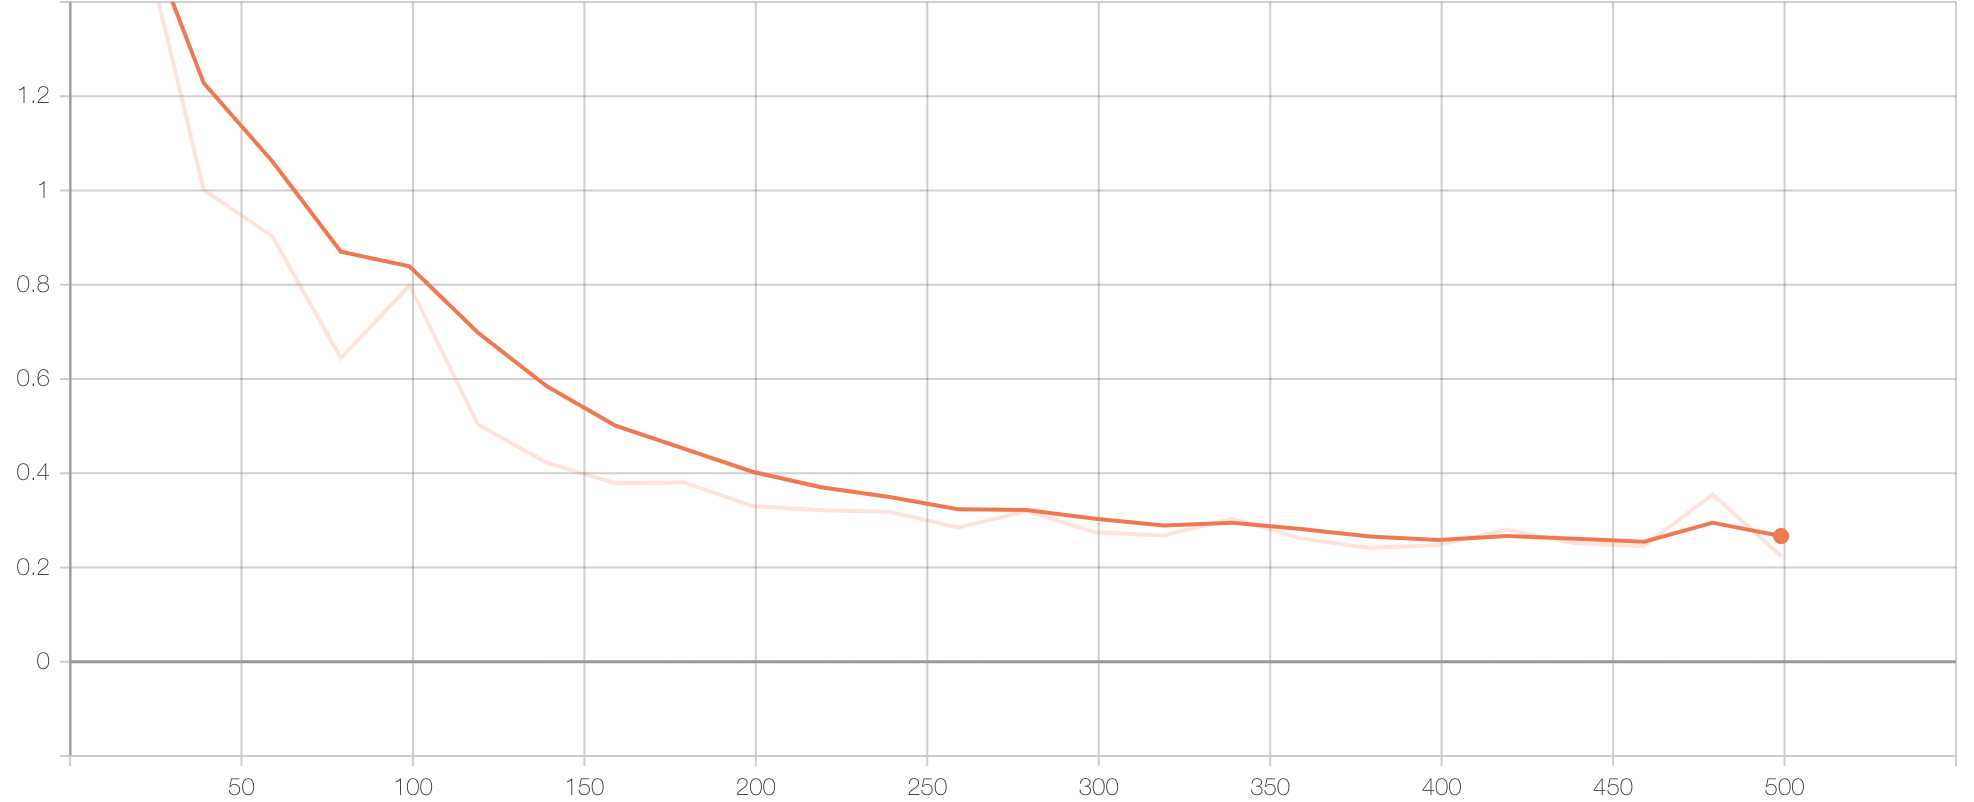
\includegraphics[scale=0.35]{figures/loss_cls_retinanet_4}
\caption{\small \sl «Loss cls», også kjent som «entropy loss», for RetinaNet-modellen. \label{fig:loss_cls_retinanet}}
\end{center}
\end{figure}

Neste graf viser utviklingen av learning rate. Learning rate går stadig nedover ettersom modellen trenes, dette gjøres med en learning rate scheduler. Dette gjøres i et forsøk på å få ned total loss.

\begin{figure}[H]
\begin{center} 
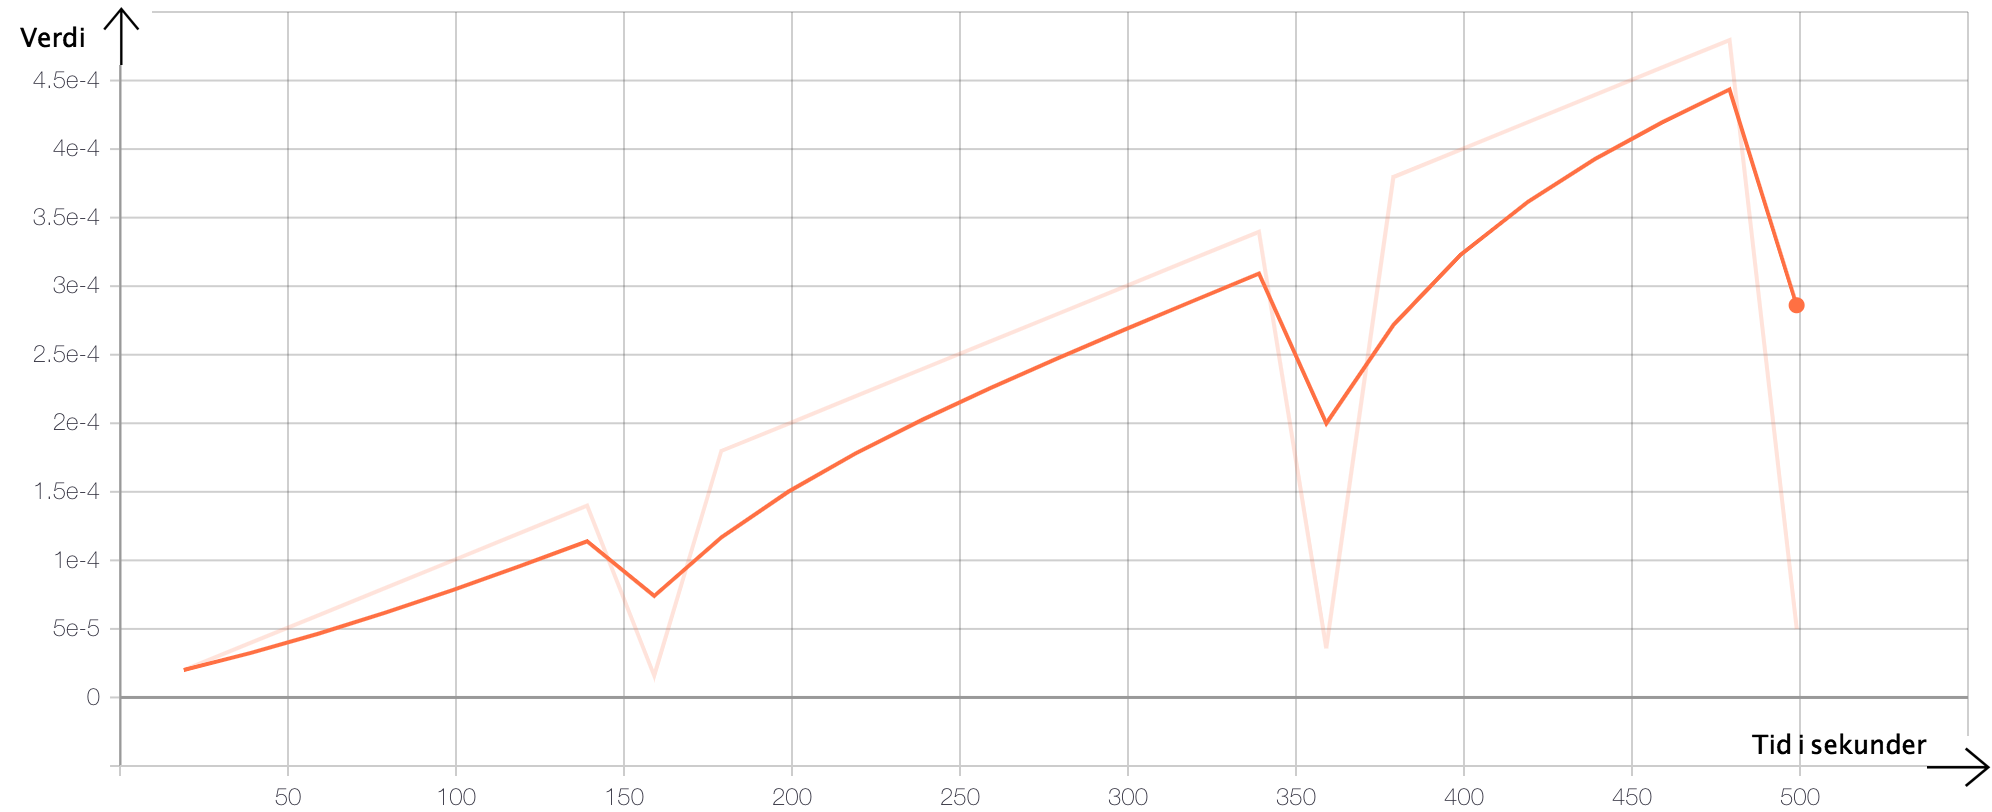
\includegraphics[scale=0.35]{figures/lr_retinanet_5}
\caption{\small \sl Utviklingen av learning rate for RetinaNet-modellen. \label{fig:lr_retinanet}}
\end{center}
\end{figure}

%\begin{figure}[h!]
%\begin{center} 
%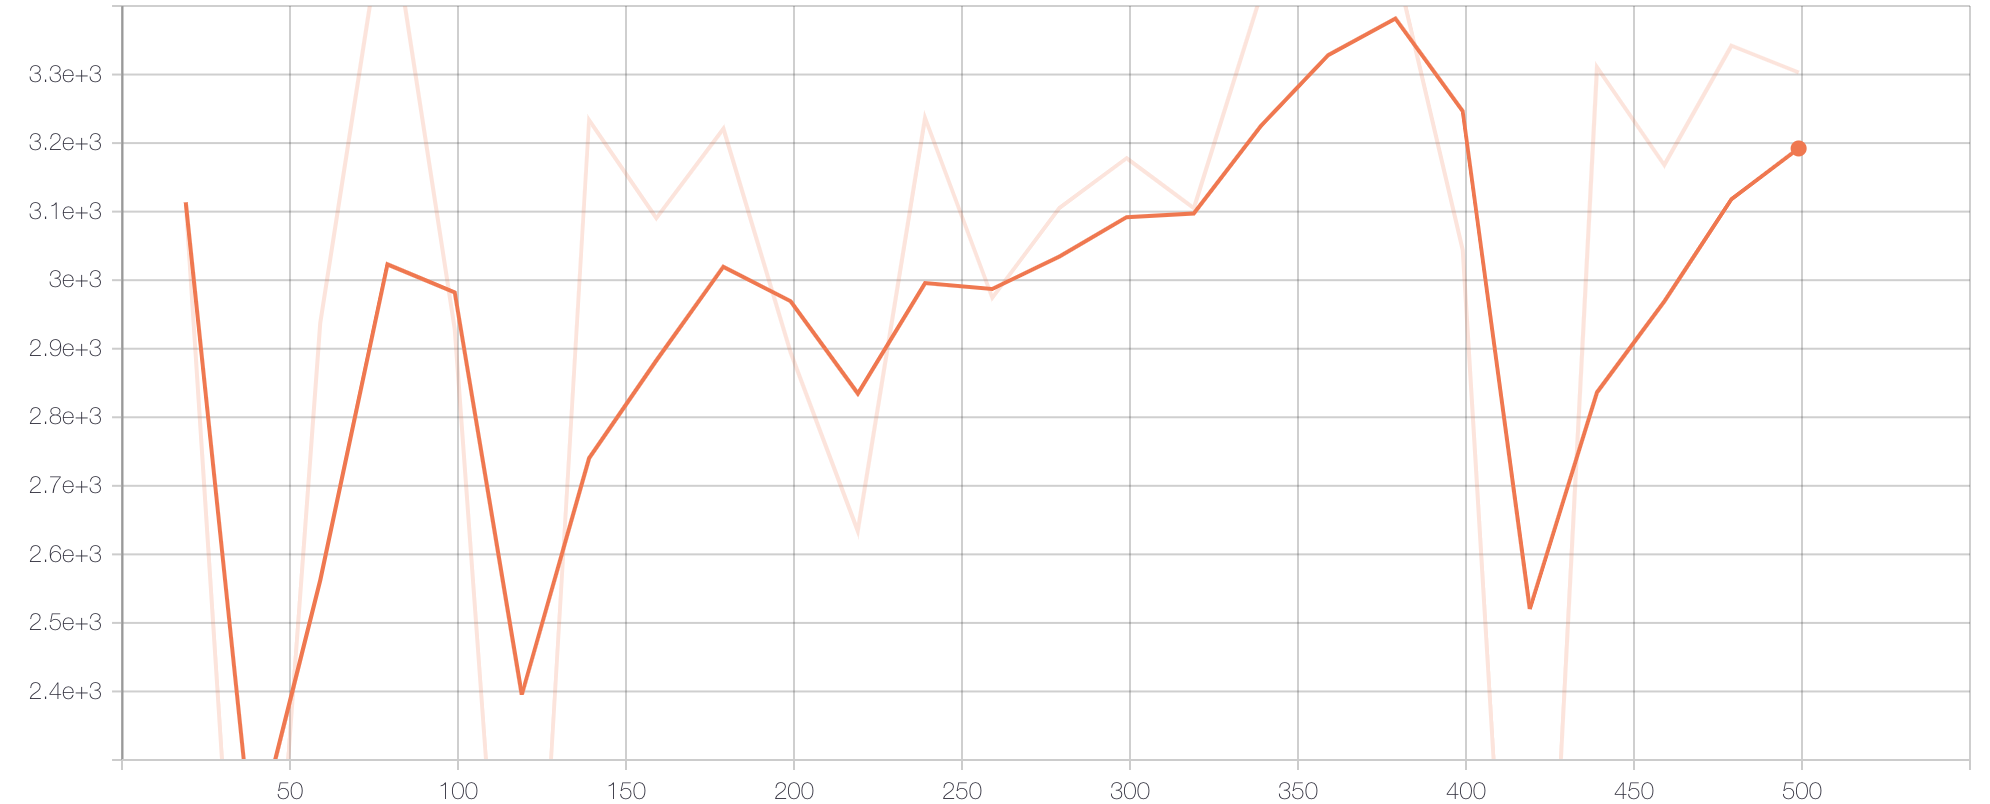
\includegraphics[scale=0.35]{figures/num_foreground_6}
%\caption{\small \sl num foreground RetinaNet. \label{fig:num_foreground}}
%\end{center}
%\end{figure}

%\begin{figure}[h!]
%\begin{center} 
%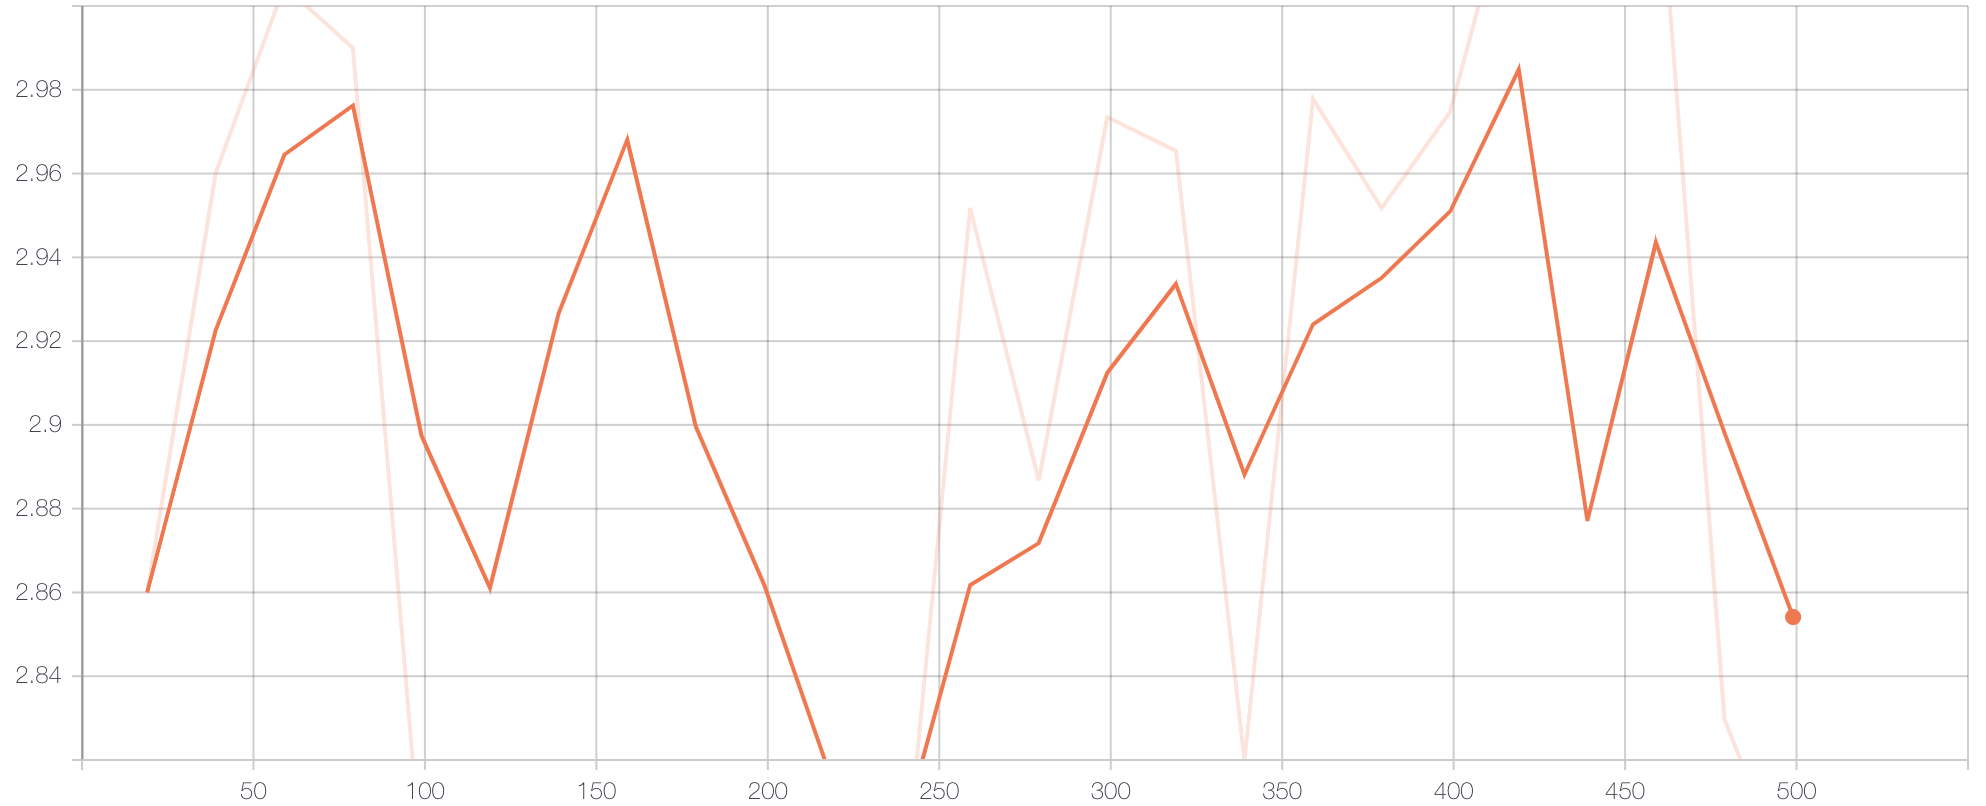
\includegraphics[scale=0.35]{figures/time_retinanet_7}
%\caption{\small \sl time RetinaNet. \label{fig:time_retinanet}}
%\end{center}
%\end{figure}

Total loss er den viktigste målingen som gjøres på deep learning-modeller. Målet med treningen av deep learning-modeller er å få total loss til å bli så lav som mulig. Den neste grafen viser utviklingen av total loss. Når modellen er ferdig trent, så vil vanligvis total loss konvergere, den blir flat. Om total loss ser ut til å fortsette å avta, så bør modellen trenes over flere iterasjoner. Learning rate har en stor innvirking på når total loss konvergerer.

\begin{figure}[H]
\begin{center} 
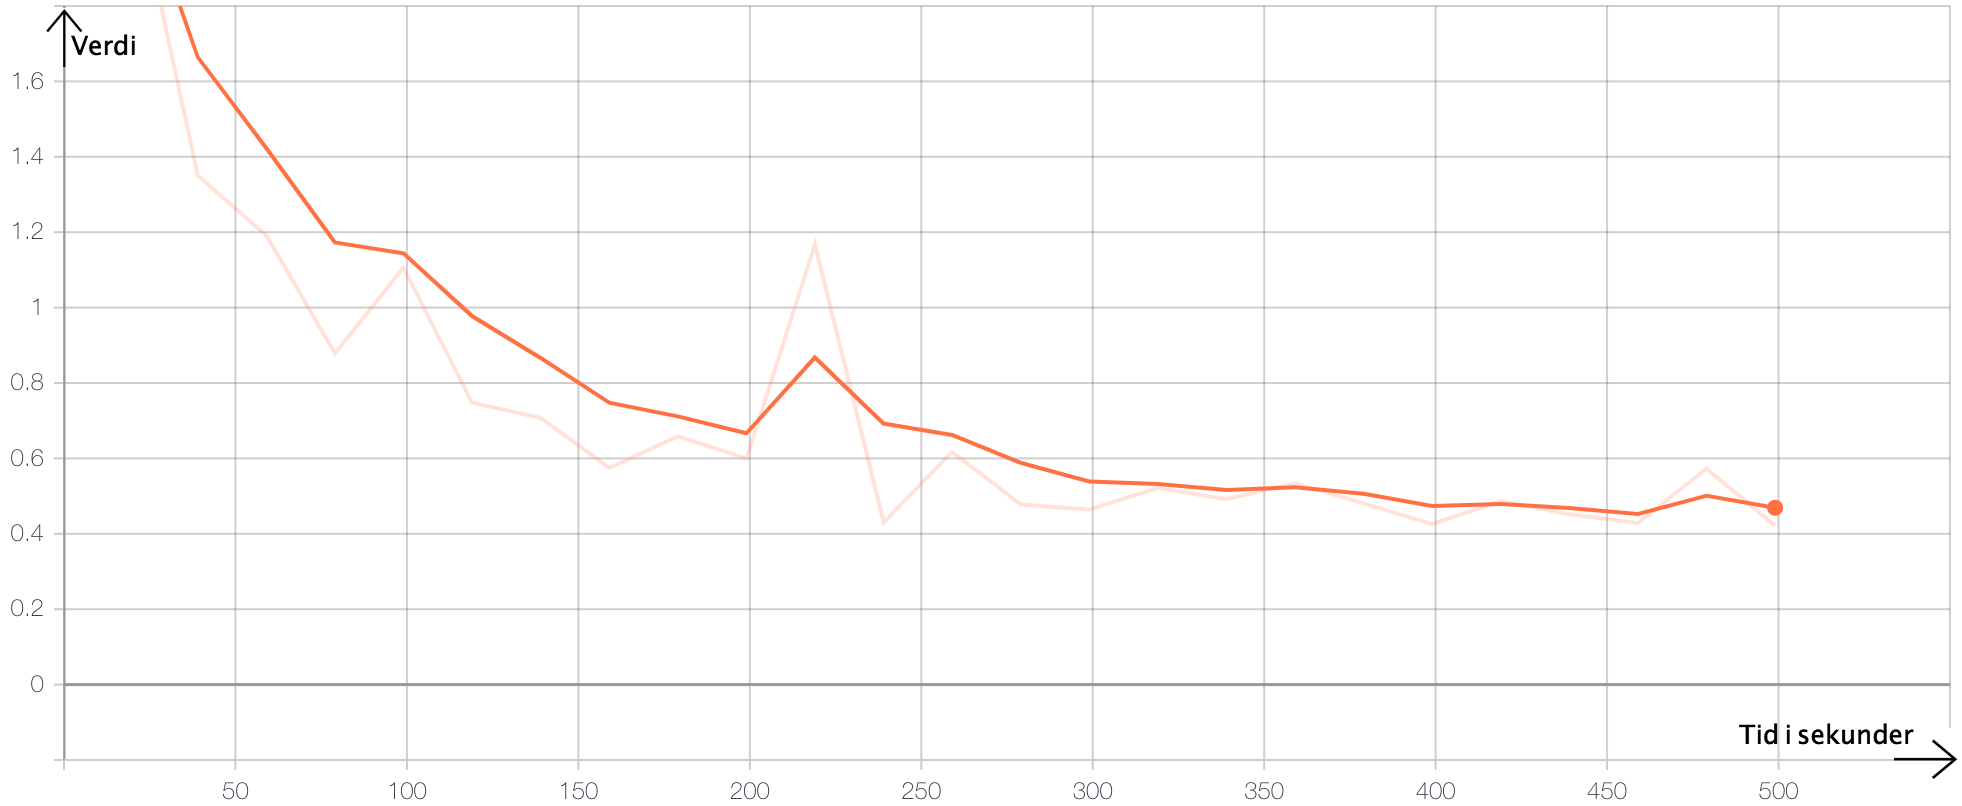
\includegraphics[scale=0.35]{figures/total_loss_retinanet_8}
\caption{\small \sl Total loss for RetinaNet-eksperimentet. \label{fig:total_loss_retinanet}}
\end{center}
\end{figure}

RetinaNet-resultatene for dette eksperimentet er også tilgjengelige på nettet.\footnote{\url{https://tensorboard.dev/experiment/2PxmdvA5QdavQC0YLABdgw}}

\subsection{YOLO}

Mean Average Precision (mAP) er gjennomsnittet av maksimumpresisjonene ved alle recall-verdiene. Denne målingen brukes til å måle hvor bra en objektdeteksjonsmodell har blitt. Når YOLOv4-modellen ble testet på datasettet så hadde modellen en mAP (mean Average Precisoin) på 73 \%. Se figur \ref{fig:chart_yolo}. Total loss gikk ned til litt over 5,5. %When tested on individual source of dataset, the model achieved best results on Wells Dam dataset with 0.5575 mAP, se figur \ref{fig:chart_yolo}. Wells Dam dataset’s better performance than the other two datasets were as expected, considering its high resolution and three full color channels. However, the mAP metric on Wells Dam dataset is lower than our expectation. Fig. 2 F reveals that most of the false detection in Wells Dam dataset are at the side of fish ladder window, where only partial of the fish bodies are visible and difficult for even human annotators to correctly label. These hard cases are sometimes more numerous than fish passing through the white plate, which greatly reduced the overall mAP score on the Wells Dam dataset. \cite{Xu og Matzner 2018}

%mAP (mean average precision) - mean value of average precisions for each class, where average precision is average value of 11 points on PR-curve for each possible threshold (each probability of detection) for the same class (Precision-Recall in terms of PascalVOC, where Precision=TP/(TP+FP) and Recall=TP/(TP+FN) ), %page-11: http://homepages.inf.ed.ac.uk/ckiw/postscript/ijcv_voc09.pdf

\begin{figure}[h!]
\begin{center} 
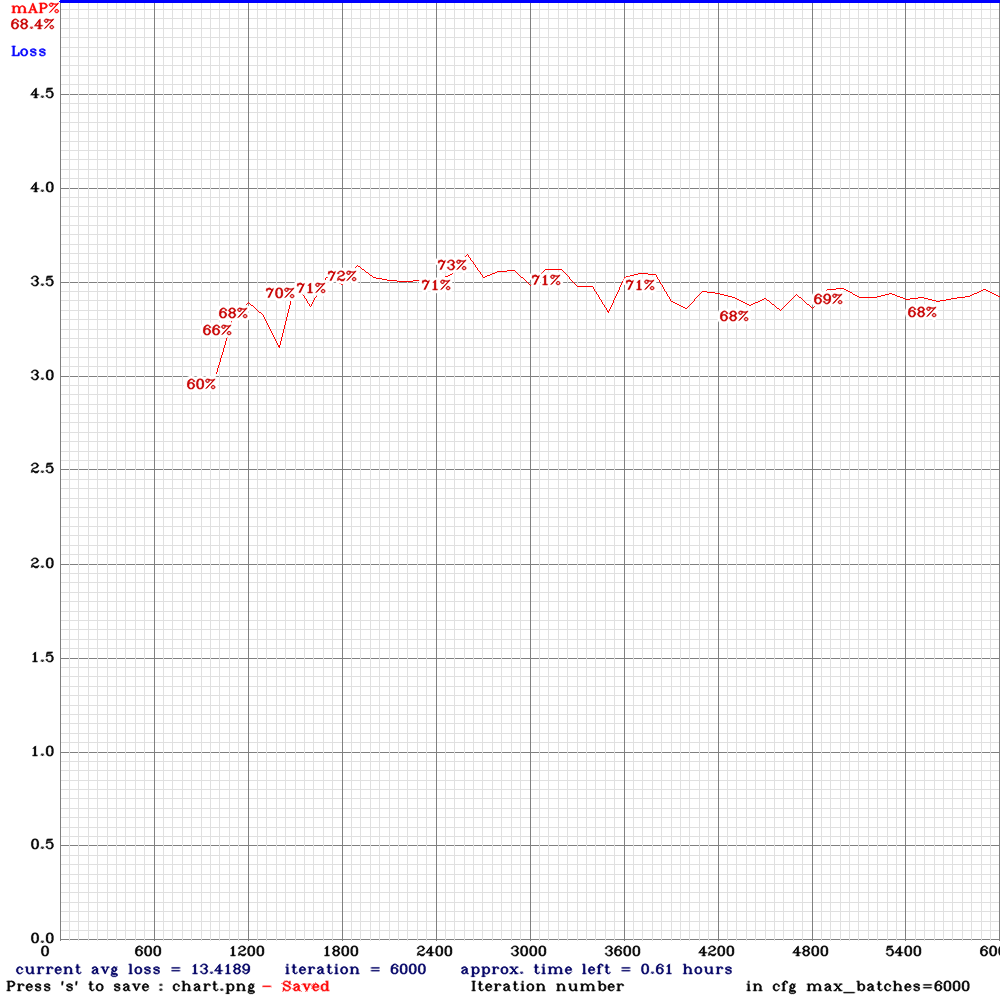
\includegraphics[scale=0.35]{figures/chart_yolo-obj.png}
\caption{\small \sl graf YOLO. \label{fig:chart_yolo}}
\end{center}
\end{figure}
% Vurdering 1/5
%Du skal her drøfte resultatene dine og sette dem inn i en sammenheng. Å drøfte vil si å:

%sette ulike synspunkter, momenter, argumenter, faktorer og årsaker opp mot hverandre
%vurdere og sette dem opp mot hverandre. Finnes det flere ulike tolkninger av resultatene?
%Du må i kapitlet svare på:

%hvordan svarer resultatene dine på forskningsspørsmålene dine?
%hva betyr resultatene?
%Et lurt tips er å gjenta forskningsspørsmålene, slik at leseren blir minnet på hva de er.

%Du skal òg se tilbake på studien og vurdere hvor gyldig og pålitelig den har vært.

%Hva kunne blitt gjort annerledes?
%Hva er sterke og svake sider?
%Her kan du for eksempel kritisere metodene som du har brukt, og forklare hva du kunne gjort annerledes.

\section{Diskusjon}
\label{part:discussion}
Datasettet burde bestå av data uten bias. Modellene som er trent kan effektivt se forskjell på torsk og sei som finnes i bildene, men ettersom bildene ble tatt på så forskjellige måter, der sei dataen var i gråtoner og torsk var i farger, så vil modellen muligens se etter fisk av gråtoner, ikke sei, når den gjør inferens. Datasettet bestod av 208 bilder av torsk, med til sammen 4582 instanser av torsk i bildene. Det var 604 bilder av sei med 5525 instanser av fisken i bildene. Det er litt flere instanser av sei enn av torsk. Det kan også øke bias i modellen i noe grad.

Det som er lettere for mennesker å forstå er også lettere for maskiner å forstå. Data is king innenfor maskinsyn, å ha gode bilder er et must for å få gode resultater. Det betyr ikke at et bilde av gråtoner, eller av lav oppløsning er dårlige. Det er faktisk mange fordeler med gråtoner og lav oppløsning. De kan prosesseres raskt, og av og til så blir de viktigste egenskapene mer synlige.

Når en modell har blitt trent ferdig bør den forbedres. Den mest effektive måten å forbedre en deep learning-modell er å endre learning rate i konfigurasjonen, og så trene modellen på nytt. Det kan også hjelpe å bruke en ny modell, vanligvis så er en modell med flere konvolveringslag bedre. Dype nevrale nettverk blir stadig dypere ettersom forskere utvikler nye modeller \cite{Szegedy m.fl. s. 1}. Det er også mulig å trene modellen over flere epoker eller iterasjoner. 

RetinaNet-modellen hadde overraskende lav Average Precision og Average Recall og kan sannsynligvis forbedres ved å trenes på nytt, for eksempel med et større antall iterasjoner eller ved å justere learning-rate. Det er alltid lurt å trene modeller flere ganger med forskjellige parametere.

YOLOv4-modellen hadde ganske gode resultater. Total loss burde egentlig være mellom 3,0 og 0,05, men endte opp på litt over 5,5. Modellen kan muligens forbedres ved å ved å justere learning rate. 

Å eksperimentere med dataaugmentering kan også føre til bedre resultater for begge modellene. Bilder kan roteres tilfeldig med og mot klokken, lysstyrken i bildene kan bli tilfeldig endret, nye bilder kan skapes med zoom og bildene kan bli snudd horisontalt og vertikalt. Støy kan legges til bildene. Disse eksperimentene kan utføres ved å konfigurere maskinlæringsrammeverkene. 

Fish4Knowledge-, LifeCLEF- og SeaCLEF-datasettene kan legges til modellen, da vil den kjenne igjen flere fiskearter.

OpenCV-programmet og YOLOv4-modellen kan testes videre, og trenes opp på data uten bias. Modellene bør testes på en videostrøm som inneholder både torsk og sei, og testes på data fra under oppdrettsanlegg for å se om den virker til den påtenkte arbeidsoppgaven den er laget for. Etter videre testing og eventuell trening på ny data så kan modellene og OpenCV-programmet bli brukt til å hjelpe oppdrettsnæringen til å ha bedre kontroll på fôringen ved å gi næringen en oversikt over mengden torsk og sei som trekker til oppdrettsanleggene.

%The most important outcome of this research is the classification accuracy achieved. With the other species class included, the accu- racy of the classification is 89.0 \%, which is competitive with or exceeds other recently reported results on fish species identifica- tion tasks (Hsiao et al., 2014; Huang et al., 2015; Salman et al., 2016). If the other species class is excluded, the classification accu- racy within the 16 species classes is 94.3 \%, which is competitive with the identification rates of human experts for similar tasks (Culverhouse et al., 2003).
%%Om avslutningen din skal være en konklusjon eller en oppsummering, avhenger av problemstillingen din. En konklusjon skal svare på problemstillingen, mens en oppsummering gjentar det viktigste fra oppgaven. Det er ikke uvanlig å velge en kombinasjon av de to, hvor du både oppsummerer oppgaven kort, men også svarer på problemstillingen.

%Det er lurt å la avslutningen speile innledningen, ved å si hva du har gjort. Avslutningen bør også sette oppgaven din i et større perspektiv, og peke på hvilke muligheter du ser ut fra ditt prosjekt. Hvilke bidrag har din undersøke gitt til faget? Er det noe som burde blitt studert ytterligere? Slik tar du utgangspunkt i ditt eget prosjekt og peker på mulighet for oppfølging.

\section{Konklusjon}

\label{part:end}

Maskinsyn kan anvendes til å hjelpe oppdrettsnæringen med å få kontroll på fôring av oppdrettfisk ved å gi industrien en tidsoversikt over mengden torsk og sei som trekker til anleggene.

Ved å tilpasse fôringen av oppdrettsfisken så vil fôrsprengt fisk bli et mindre problem. Kunnskapen som kan samles med automatisk videoanalyse kan hjelpe de marine næringene med å leve godt sammen langs kysten.

Maskinlæringsmodellene kan utvikles videre. En forbedret modell vil kunne gi oppdrettsnæringen en enda bedre tidsoversikt over torsk og sei under oppdrettsanleggene.

Et forbedret datasett, med flere fiskearter og mindre bias vil også forbedre resultatene. Automatisk analyse av undervannsvideoer kan gi forskere regelmessig informasjon om de marine økosystemene. Det er viktig å ha denne informasjonen når en gjør avgjørelser som kan påvirke miljøet og økonomien til de marine næringene.


\begin{thebibliography}{9}

% 137 ABCDEFGHIJKLMNOPQRSTUVXYZ

\bibitem{Angell og Ekanger 2017} 
Angell E., og Ekanger A. 
\textit{Fekk fisk med magen full av oppdrettsfôr}. 
NRK, \url{https://www.nrk.no/vestland/fekk-fisk-med-magen-full-av-oppdrettsfor-1.13677856}, 2017. (hentet 24. April 2020)

\bibitem{Batanina 2020} 
Batanina L.
\textit{Feature-request: State-of-art Yolo v4 Detector}. 
Github \url{https://github.com/opencv/opencv/issues/17148}, 2020. (hentet 6. Mai 2020)

\bibitem{Bochkovskiy 2020} 
Bochkovskiy A.
\textit{YOLOv4 (v3/v2)}. 
Github \url{https://github.com/AlexeyAB/darknet}, 2020. (hentet 6. Mai 2020)

\bibitem{Bochkovskiy m.fl. 2020} 
Bochkovskiy A, Wang C.Y., og Liao H.Y. M.
\textit{YOLOv4: Optimal Speed and Accuracy of Object Detection}. 
arXiv.org \url{https://arxiv.org/abs/2004.10934}, 2020. (hentet 8. Mai 2020)

\bibitem{IanBuck} 
Buck I.
\textit{Stream Computing on Graphics Hardware}. 
Stanford University \url{http://graphics.stanford.edu/~ianbuck/thesis.pdf}, 2006. (hentet 6. Mai 2020)

\bibitem{Baevre-Jensen 2019} 
Bævre-Jensen M.
\textit{Kostnadene for norsk lakseoppdrett fortsetter å øke også i 2019}. 
Fiskeri- og havbruksnæringens forskningsfinansiering (FHF) \url{https://www.fhf.no/nyheter/nyhetsarkiv/kostnadene-for-norsk-lakseoppdrett-fortsetter-aa-oeke-ogsaa-i-2019}, 2019. (hentet 6. Mai 2020)

\bibitem{primate} 
Cadieu C. F., Hong H., Yamins D. L. K., Pinto N., Ardila D., Solomon E. A., Majaj N. J., og DiCarlo J. J. 
\textit{Deep Neural Networks Rival the Representation of Primate IT Cortex for Core Visual Object Recognition}. 
PLOS Computational Biology, 2014.

\bibitem{Canziani m.fl 2017} 
Canziani A., Culurciello E., og Paszke A. 
\textit{An Analysis of Deep Neural Network Models for Practical Applications}. 
Weldon School of Biomedical Engineering Purdue University, Faculty of Mathematics, Informatics and Mechanics University of Warsaw, 2017.

\bibitem{Christensen 2019} 
Christensen T. B. 
\textit{Fôrer villfisk med lusegift og medisiner}. 
Naturvernforbundet, \url{https://naturvernforbundet.no/naturogmiljo/forer-villfisk-med-lusegift-og-medisiner-article39320-1024.html}, 2019. (hentet 24. April 2020)

\bibitem{deepfish} 
Cui S., Zhou Y., Wang Y., og Zhai L. 
\textit{Fish Detection Using Deep Learning}. 
Applied Computational Intelligence and Soft Computing, 2020.

\bibitem{distributed} 
Dean J., Corrado G. S., Monga R., Chen K., Devin M., Le Q. V., Mao M. Z., Ranzato M., Senior A., Tucker P., Yang K., og Ng A. Y. 
\textit{Large Scale Distributed Deep Networks}. 
Google Inc., Mountain View, CA, 2012.

\bibitem{math} 
Dumoulin V., og Visin F. 
\textit{A guide to convolution arithmetic for deep learning}. 
MILA, Université de Montréal, AIRLab, Politecnico di Milano, 2018.

\bibitem{Falstad 2016} 
Falstad S. V.
\textit{Suksess med vaksinemaskin}. 
Trønder-avisa \url{https://www.t-a.no/nyheter/2016/02/01/Suksess-med-vaksinemaskin-12104745.ece}, 2016. (hentet 6. Mai 2020)

\bibitem{Fenstad 2019} 
Fenstad A.
\textit{Nå kan maskinen skille mellom makrell og sild}. 
tu.no \url{https://www.tu.no/artikler/na-kan-maskinen-skille-mellom-makrell-og-sild/464208?utm_source=newsletter-tudaily&utm_medium=email&utm_campaign=newsletter-2019-05-06}, 2019. (hentet 6. Mai 2020)

\bibitem{Girshick 2015} 
Girshick R. 
\textit{Fast R-CNN}. 
Microsoft Research, 2015.

\bibitem{semantic_segmentation} 
Girshick R., Donahue J., Darrell T., og Malik J. 
\textit{Rich feature hierarchies for accurate object detection and semantic segmentation}. 
UC Berkeley, 2014.

\bibitem{Goodfellow m.fl. 2016} 
Goodfellow I., Bengio Y., og Courville A. 
\textit{Deep Learning}. 
MIT Press \url{www.deeplearningbook.org}, 2016. (hentet 26. April 2020)

\bibitem{resnet} 
He K., Zhang X., Ren S., og Sun J. 
\textit{Deep Residual Learning for Image Recognition}. 
Microsoft Research, 2015.

\bibitem{stochastic_depth} 
Huang G., Sun Y., Liu Z., Sedra D., og Weinberger K. Q. 
\textit{Deep Networks with Stochastic Depth}. 
Cornell University, Tsinghua University, 2016.

\bibitem{hubel} 
Hubel D. H., og Wiesel T. N. 
\textit{Receptive Fields of Single Neurones in the Cat's Striate Cortex}. 
 Wilmer Institute, The Johns Hopkins Hospital and University, Baltimore, Maryland, U.S.A., 1959.
 
\bibitem{Hustad og Svalheim 2020} 
Hustad A., og Svalheim R.
\textit{Hvem bryr seg om pelletssei?}. 
Nofima \url{https://www.fhf.no/nyheter/nyhetsarkiv/kostnadene-for-norsk-lakseoppdrett-fortsetter-aa-oeke-ogsaa-i-2019}, 2019. (hentet 6. Mai 2020)

\bibitem{batchnorm} 
Ioffe S., og Szegedy C. 
\textit{Batch Normalization: Accelerating Deep Network Training by Reducing Internal Covariate Shift}. 
Google Inc, 2015.

\bibitem{Jakobsen 2017} 
Jakobsen A. N.
\textit{Fikk torsk full av oppdrettsfôr: – Motbydelig fisk}. 
NRK, \url{https://www.nrk.no/tromsogfinnmark/fikk-torsk-full-av-oppdrettsfor_-_-motbydelig-fisk-1.13662637}, 2017. (hentet 24. April 2020)

\bibitem{seaclef} 
Jäger J., Rodner E., Denzler J., Wolff V., og Fricke-Neuderth K. 
\textit{SeaCLEF 2016: Object proposal classification for fish detection in underwater videos}. 
Department of Electrical Engineering and Information Technology, Fulda University of Applied Sciences, Germany, Computer Vision Group, Friedrich Schiller University Jena, Germany, 2016.

\bibitem{captioning} 
Johnson J., Karpathy A., og Fei-Fei L. 
\textit{DenseCap: Fully Convolutional Localization Networks for Dense Captioning}. 
Department of Computer Science, Stanford University, 2015.

\bibitem{andrej} 
Karpathy A. 
\textit{Convolutional Neural Networks}. 
Stanford University \url{https://www.youtube.com/watch?v=bNb2fEVKeEo}, 2014. (hentet 13. mai 2020)

\bibitem{ImageNet} 
Krizhevsky A., Sutskever  I., og Hinton G. E.. 
\textit{ImageNet Classification with Deep Convolutional Neural Networks}. 
University of Toronto, 2012.

\bibitem{docreg} 
LeCun Y., Bottou L., Bengio Y., og Haner P. 
\textit{Gradient-Based Learning Applied to Document Recognition}. 
IEEE, 1998.

\bibitem{coco} 
Lin T.Y., Maire M., Belongie S., Bourdev L., Girshick R., Hays J., Perona P., Ramanan D., Zitnick C. L., og Dollár P. 
\textit{Microsoft COCO: Common Objects in Context}. 
Microsoft, 2015.

\bibitem{retinanet} 
Lin T.Y., Goyal P., Girshick R., He K., Dollár P.
\textit{Focal Loss for Dense Object Detection}
Facebook AI Research, 2018.

\bibitem{Mallick m.fl. 2020} 
Mallick S., Gupta V., Murzova A., Petrovicheva A., Serebryakov G., Semkin P., Chandra P., Belousov S., Khanova T., og Koriukina V.
\textit{Deep Learning with PyTorch}. 
OpenCV.org \url{https://courses.opencv.org}, 2020. (hentet 14. Mai 2020)

\bibitem{Nielsen 2019} 
Nielsen M. 
\textit{Using neural nets to recognize handwritten digits}. 
\url{http://neuralnetworksanddeeplearning.com/chap1.html}, 2019. (hentet 28. April 2020)

\bibitem{nrk 2018} 
NRK. 
\textit{Laks med medisinrester har rømt fra Marine Harvest-anlegg}. 
NRK, \url{https://www.nrk.no/trondelag/laks-har-romt-fra-marine-harvest-anlegg-i-naeroy-1.13902322}, 2019. (hentet 25. April 2020)

\bibitem{Olsen 2019} 
Olsen J. E. 
\textit{Ny oppmerksomhet rundt “pellets-fisken”}. 
fiskeribladet, \url{https://fiskeribladet.no/nyheter/?artikkel=69867}, 2019. (hentet 24. April 2020)

\bibitem{Olsen m.fl. 2018} 
Olsen O.C., Johansen J. I., og Grov B. 
\textit{Villfisk mettes av oppdrettsmat: – Jeg blir rett og slett forbanna}. 
NRK, \url{https://www.nrk.no/nordland/villfisk-mettes-av-oppdrettsmat_-_-jeg-blir-rett-og-slett-forbanna-1.14003547}, 2018. (hentet 24. April 2020)

\bibitem{OpenCV Team 2020} 
OpenCV Team. 
\textit{About OpenCV}. 
OpenCV \url{https://opencv.org/about/}, 2020. (hentet 5. Mai 2020)

\bibitem{Redmon 2016} 
Redmon J. 
\textit{Darknet: Open Source Neural Networks in C}. 
\url{http://pjreddie.com/darknet/}, 2013-2016.

\bibitem{Redmon 2018} 
Redmon J. 
\textit{YOLOv3: An Incremental Improvement}. 
arXiv, 2018.

\bibitem{Ren m.fl. 2016} 
Ren S., He K., Girshick R., og Sun J.
\textit{Faster R-CNN: Towards Real-Time Object Detection with Region Proposal Networks}. 
University of Science and Technology of China, Microsoft Research, 2016.

\bibitem{Robertsen 2020} 
Robertsen R. 
\textit{Sameksistens av marine næringer i kystsonen}. 
Nofima, \url{https://nofima.no/prosjekt/sameksistens}, 2020.

\bibitem{marinescience} 
Salman A, Siddiqui S. A. , Shafait F., Mian A., Shortis M. R., Khurshid K., Ulges A., og Schwanecke U. 
\textit{Automatic fish detection in underwater videos by a deep neural network-based hybrid motion learning system}. 
ICES Journal of Marine Science, 2019.

\bibitem{entropy} 
Shannon C. E. 
\textit{A Mathematical Theory of Communication}. 
Bell Labs, 1948.

\bibitem{Szegedy m.fl. 2014} 
Szegedy C., Liu W., Jia Y., Sermanet P., Reed S., Anguelov D., Erhan D., Vanhoucke V., og Rabinovich A. 
\textit{Going deeper with convolutions}. 
Google Inc., University of Michigan, University of North Carolina, Chapel Hill, arXiv, 2014.

\bibitem{Debt} 
Sculley D., Holt G., Golovin D., Davydov E., Phillips T., Ebner D., Chaudhary V., Young M., Crespo J.F., og Dennison D. 
\textit{Hidden Technical Debt in Machine Learning Systems}. 
Google Inc., 2015.

\bibitem{autofish} 
Siddiqui S. A., Shafait F., Mian A. S., og Shortis M. R. 
\textit{Automatic fish species classification in underwater videos: Exploiting pretrained deep neural network models to compensate for limited labelled data}. 
ICES Journal of Marine Science, 2017.

\bibitem{vgg} 
Simonyan K., og Zisserman A. 
\textit{Very Deep Convolutional Networks for Large-Scale Image Recognition}. 
Visual Geometry Group, Department of Engineering Science, University of Oxford, 2015.

\bibitem{texton_forests} 
Shotton J., Johnson M., og Cipolla R. 
\textit{Semantic Texton Forests for Image Categorization and Segmentation}. 
Toshiba Corporate R\&D Center Kawasaki, Japan, Department of Engineering University of Cambridge, UK, 2008.

\bibitem{Spruill 2011} 
Spruill V.
\textit{Environmental Impacts of Open-Ocean Aquaculture}. 
Ocean Conservancy \url{https://issuu.com/oceanconservancy/docs/oc_rfts_v11_single}, 2011. (hentet 6. Mai 2020)

\bibitem{Saether 2017} 
Sæther B.S. 
\textit{Effekter av oppdrett på vill marin fisk}. 
Nofima, \url{https://nofima.no/nyhet/2017/09/effekter-av-oppdrett-pa-vill-marin-fisk/}, 2017. (hentet 24. April 2020)

\bibitem{The Apache Software Foundation 2004} 
The Apache Software Foundation 
\textit{Apache License, Version 2.0}. 
The Apache Software Foundation \url{https://www.apache.org/licenses/LICENSE-2.0}, 2004. (hentet 5. Mai 2020)

\bibitem{Trana m.fl. 2019} 
Trana K., Klausen D. H., og Bolstad J. 
\textit{Denne torsken er full av fôr fra oppdrettsnæringa}. 
NRK, \url{https://www.nrk.no/trondelag/fiskere-har-solgt-torsk-som-er-full-av-lakselusmiddel-_-vet-ikke-om-det-er-farlig-1.14742706}, 2019. (hentet 24. April 2020)

\bibitem{Wu2020} 
Wu Y., Kirillov A., Massa F., Lo W.Y., og Girshick R.
\textit{Detectron2}. 
Github \url{https://github.com/facebookresearch/detectron2}, 2020. (hentet 6. Mai 2020)

\bibitem{KentaroWada2020} 
Wada K.
\textit{labelme: Image Polygonal Annotation with Python}. 
Github \url{https://github.com/wkentaro/labelme}, 2016. (hentet 6. Mai 2020)

\bibitem{underwater} 
Xu W., og Matzner S. 
\textit{Underwater Fish Detection using Deep Learning for Water Power Applications}. 
Pacific Northwest National Laboratory, 2018.

\bibitem{yang} 
Yang M. Y., og Förstner W. 
\textit{A Hierarchical Conditional Random Field Model for Labeling and Classifying Images of Man-made Scenes}. 
Department of Photogrammetry, Institute of Geodesy and Geoinformation, University of Bonn Nussallee 15, 53115 Bonn, Germany, 2011.

%https://gilberttanner.com/blog/detectron2-train-a-instance-segmentation-model

\end{thebibliography}

\clearpage
\appendix
\pagenumbering{arabic}
\setcounter{page}{1}

\pagestyle{fancy}
%\fancyhf{}
\rhead{Vedlegg A side \thepage}
%\lhead{Guides and tutorials}

\section{Kildekode}
\label{appendix:code}

\begin{lstlisting}[language=Python, caption=Her lastes bibliotekene inn i train.py for detectron2,label={lst:load}]
import torch
import detectron2
#import onnx
#from detectron2 import export
from detectron2.utils.logger import setup_logger
setup_logger()

# import some common libraries
import numpy as np
import cv2
import random
import os
import matplotlib.pyplot as plt

# model_zoo has a lots of pre-trained model
from detectron2 import model_zoo


# DefaultTrainer is a class for training object detector
from detectron2.engine import DefaultTrainer
# DefaultPredictor is class for inference
from detectron2.engine import DefaultPredictor

# detectron2 has its configuration format
from detectron2.config import get_cfg
# detectron2 has implemented Visualizer of object detection
from detectron2.utils.visualizer import Visualizer

# from DatasetCatalog, detectron2 gets dataset and from MetadatCatalog it
# gets metadata of the dataset
from detectron2.data import DatasetCatalog, MetadataCatalog

# BoxMode support bounding boxes in different format
from detectron2.structures import BoxMode

# COCOEvaluator based on COCO evaluation metric, inference_on_dataset is used for
# evaluation for a given metric
from detectron2.evaluation import COCOEvaluator, inference_on_dataset

# build_detection_test_loader, used to create test loader for evaluation
from detectron2.data import build_detection_test_loader

\end{lstlisting}

%\begin{lstlisting}[language=Python, caption=Treningen og testingen, samt operativssystemet konfigureres]
\begin{lstlisting}[language=Python, caption=Konfigurasjon i train.py,label={lst:config}]
data_root = 'data'
train_txt = 'fish_train.txt'
test_txt  = 'fish_test.txt'

train_data_name = 'fish_train'
test_data_name  = 'fish_test'

thing_classes = ['atlantic_cod', 'saithe']

output_dir = 'outputs'

def count_lines(fname):
    with open(fname) as f:
        for i, l in enumerate(f):
            pass
    return i + 1

train_img_count = count_lines(os.path.join(data_root, train_txt))

# Register train and test data
# dataset can be registered only once with one name

# register train data
DatasetCatalog.register(name=train_data_name,
                        func=lambda: get_fish_dicts(data_root, train_txt))
train_metadata = MetadataCatalog.get(train_data_name).set(thing_classes=thing_classes)

# register test data
DatasetCatalog.register(name=test_data_name,
                        func=lambda: get_fish_dicts(data_root, test_txt))
test_metadata = MetadataCatalog.get(test_data_name).set(thing_classes=thing_classes)

# default configuration
cfg = get_cfg()

# update configuration with RetinaNet configuration
cfg.merge_from_file(model_zoo.get_config_file("COCO-Detection/retinanet_R_50_FPN_3x.yaml"))
cfg.MODEL.ROI_HEADS.SCORE_THRESH_TEST = 0.5

# We have registered the train and test data set with name fish_train and fish_test.
# Let's replace the detectron2 default train dataset with our train dataset.
cfg.DATASETS.TRAIN = (train_data_name,)

# No metric implemented for the test dataset, we will have to update
# cfg.DATASET.TEST with empty tuple
cfg.DATASETS.TEST = ()

# data loader configuration
cfg.DATALOADER.NUM_WORKERS = 4

# Update model URL in detectron2 config file
cfg.MODEL.WEIGHTS = model_zoo.get_checkpoint_url("COCO-Detection/retinanet_R_50_FPN_3x.yaml")
model_final_f10217.pkl"
\end{lstlisting}

\begin{lstlisting}[language=Python, caption=Inferens RetinaNet i inference.py,label={lst:inferens_retinanet}]
def video_read_write(video_path):
    """
    Read video frames one-by-one, flip it, and write in the other video.
    video_path (str): path/to/video
    """
    video = cv2.VideoCapture(video_path)
    
    # Check if camera opened successfully
    if not video.isOpened(): 
        print("Error opening video file")
        return
    
    # create video writer
    width = int(video.get(cv2.CAP_PROP_FRAME_WIDTH))
    height = int(video.get(cv2.CAP_PROP_FRAME_HEIGHT))
    frames_per_second = video.get(cv2.CAP_PROP_FPS)
    num_frames = int(video.get(cv2.CAP_PROP_FRAME_COUNT))
    
    isStreamOpen = False
    while video.isOpened():
        ret, frame = video.read()
        
        if ret:
            outputs = predictor(frame)

            #print(outputs)
            v = Visualizer(frame[:, :, ::-1],
                           metadata=test_metadata, 
                           scale=0.8
            )

            instances = outputs["instances"].to("cpu")

            v = v.draw_instance_predictions(instances)

            plt.imsave('outputs/frame_intermediate.png', v.get_image())

            if isStreamOpen == False:
                img = cv2.imread('outputs/frame_intermediate.png')
                height, width, layers = img.shape
                size = (width,height)
                out = cv2.VideoWriter('out.avi',cv2.VideoWriter_fourcc(*'DIVX'),
                		      frames_per_second, size)
                isStreamOpen = True

            img = cv2.imread('outputs/frame_intermediate.png')

            cv2.putText(img, 'num instances: ' + str(len(instances)), (5,100),
            		cv2.FONT_HERSHEY_SIMPLEX, 3, (0, 255, 0), 2, cv2.LINE_AA)
            out.write(img)

            print ('num instances: ' + str(len(instances)))
        else:
            break
    
    out.release()
    video.release()
    
    return

cfg.DATASETS.TEST = (test_data_name,)

# create a predictor instance with the configuration (it has our fine-tuned model)
# this predictor does prdiction on a single image
predictor = DefaultPredictor(cfg)

# create directory for evaluation
eval_dir = os.path.join(cfg.OUTPUT_DIR, 'coco_eval')
os.makedirs(eval_dir, exist_ok=True)

# create evaluator instance with coco evaluator
evaluator = COCOEvaluator(dataset_name=test_data_name,
                          cfg=cfg,
                          distributed=False,
                          output_dir=eval_dir)

# create validation data loader
val_loader = build_detection_test_loader(cfg, test_data_name)

# start validation 
inference_on_dataset(trainer.model, val_loader, evaluator)

# Run inference on video
video_read_write('in.mp4')
\end{lstlisting}

\begin{lstlisting}[language=, caption=CMakeLists.txt,label={lst:cmake}]
cmake_minimum_required(VERSION 2.8.12)

PROJECT(app)
SET(CMAKE_CXX_STANDARD 14)

SET(Python2_ROOT_DIR ${PYTHONHOME})

find_package(Python2 COMPONENTS Development NumPy)

SET(OpenCV_DIR C:/opencv-3.4/opencv/build)

if( UNIX )
    include_directories(~/anaconda2/include/python2.7 ~/anaconda2/lib/python2.7/\
    site-packages/numpy/core/include/ ~/anaconda2/include)
else()
    include_directories(${PYTHON_INCLUDE_DIRS} ~/Anaconda2/Lib/site-packages/numpy/core/\
    	include)
endif()

if(MSVC)
SET(CMAKE_CXX_FLAGS_RELEASE "${CMAKE_CXX_FLAGS_RELEASE} /MT")
endif()

find_package( OpenCV REQUIRED )

set(OpenCV_STATIC ON) # Easier to share binaries

include_directories( ${OpenCV_INCLUDE_DIRS} )

# If the package has been found, several variables will
# be set, you can find the full list with descriptions
# in the OpenCVConfig.cmake file.
# Print some message showing some of them
message(STATUS "OpenCV library status:")
message(STATUS "    config: ${OpenCV_DIR}")
message(STATUS "    version: ${OpenCV_VERSION}")
message(STATUS "    libraries: ${OpenCV_LIBS}")
message(STATUS "    include path: ${OpenCV_INCLUDE_DIRS}")

add_executable(OBJECT_DETECTOR main.cpp)
target_include_directories(OBJECT_DETECTOR PRIVATE ${PYTHON2_INCLUDE_DIRS} \
	${PYTHON2_NUMPY_INCLUDE_DIRS})
target_link_libraries(OBJECT_DETECTOR PRIVATE ${OpenCV_LIBS} Python2::Python )

add_executable(DATASET_TOOL datasettool.cpp)
target_include_directories(DATASET_TOOL PRIVATE ${PYTHON2_INCLUDE_DIRS}\
	 ${PYTHON2_NUMPY_INCLUDE_DIRS})
target_link_libraries(DATASET_TOOL PRIVATE ${OpenCV_LIBS} Python2::Python )
\end{lstlisting}

\begin{lstlisting}[language=C++, caption=main.cpp,label={lst:header}]
#include <opencv2/opencv.hpp>
#include <opencv2/dnn.hpp>
//#include <opencv2/tracking.hpp>
#include <fstream>
//#include "matplotlibcpp.h"
#include <chrono>
#include <ctime>

using namespace std;
//using namespace matplotlibcpp;
using namespace cv::dnn;
using namespace cv;

// globals
float objectnessThreshold; // Objectness threshold
float confThreshold; // Confidence threshold
float nmsThreshold;  // Non-maximum suppression threshold
int inpWidth;  // Width of network's input image
int inpHeight; // Height of network's input image
vector<string> classes;

vector<Rect2d> bboxes;
int codQuantity, saitheQuantity;

string objectLabel;

const char *WINDOW_TITLE = "Press ESC to quit";
\end{lstlisting}

\begin{lstlisting}[language=C++, caption=main.cpp,label={lst:getOutputsNames}]
// Get the names of the output layers
auto getOutputsNames(const Net& net)
{
    static vector<String> names;
    if (names.empty())
    {
        // Get the indices of the output layers, i.e. the layers with unconnected outputs
        vector<int> outLayers = net.getUnconnectedOutLayers();

        // Get the names of all the layers in the network
        vector<String> layersNames = net.getLayerNames();

        // Get the names of the output layers in names
        names.resize(outLayers.size());
        for (size_t i = 0; i < outLayers.size(); ++i)
            names[i] = layersNames[outLayers[i] - 1];
    }
    return names;
}
\end{lstlisting}

\begin{lstlisting}[language=C++, caption=main.cpp,label={lst:drawPred}]
// Draw the predicted bounding box
void drawPred(int classId, float conf, int left, int top, int right, int bottom, Mat& frame)
{
    // Draw a rectangle displaying the bounding box
    rectangle(frame, Point(left, top), Point(right, bottom), Scalar(255, 178, 50), 3);

    // Get the label for the class name and its confidence
    string label = format("%.1f", conf * 100);
    if (!classes.empty())
    {
        CV_Assert(classId < (int)classes.size());
        label = classes[classId] + " " + label + "\%";
    }

    // Display the label at the top of the bounding box
    int baseLine;
    Size labelSize = getTextSize(label, FONT_HERSHEY_SIMPLEX, 0.5, 1, &baseLine);
    top = max(top, labelSize.height);
    rectangle(frame,
    		   Point(left, top - round(1.5*labelSize.height)),
		   Point(left + round(1.5*labelSize.width),
		   top + baseLine),
		   Scalar(255, 255, 255),
		   FILLED);
    putText(frame, label, Point(left, top), FONT_HERSHEY_SIMPLEX, 0.75, Scalar(0,0,0),1);

    objectLabel = label;
}
\end{lstlisting}

\begin{lstlisting}[language=C++, caption=main.cpp,label={lst:postprocess}]
// Remove the bounding boxes with low confidence using non-maxima suppression
void postprocess(Mat& frame, const vector<Mat>& outs)
{
    vector<int> classIds;
    vector<float> confidences;
    vector<Rect> boxes;

    codQuantity = 0;
    saitheQuantity = 0;

    for (size_t i = 0; i < outs.size(); ++i)
    {
        // Scan through all the bounding boxes output from the network and keep only the
        // ones with high confidence scores. Assign the box's class label as the class
        // with the highest score for the box.
        float* data = (float*)outs[i].data;
        for (int j = 0; j < outs[i].rows; ++j, data += outs[i].cols)
        {
            Mat scores = outs[i].row(j).colRange(5, outs[i].cols);
            Point classIdPoint;
            double confidence;
            // Get the value and location of the maximum score
            minMaxLoc(scores, 0, &confidence, 0, &classIdPoint);

            if (confidence > confThreshold)
            {
                if (classes[classIdPoint.x] == "atlantic cod") {
                    codQuantity++;
                }
                else if (classes[classIdPoint.x] == "saithe")
                {
                    saitheQuantity++;
                }

                int centerX = (int)(data[0] * frame.cols);
                int centerY = (int)(data[1] * frame.rows);
                int width = (int)(data[2] * frame.cols);
                int height = (int)(data[3] * frame.rows);
                int left = centerX - width / 2;
                int top = centerY - height / 2;

                classIds.push_back(classIdPoint.x);
                confidences.push_back((float)confidence);
                boxes.push_back(Rect(left, top, width, height));
            }
        }
    }

    // Perform non maximum suppression to eliminate redundant overlapping boxes with
    // lower confidences
    vector<int> indices;
    NMSBoxes(boxes, confidences, confThreshold, nmsThreshold, indices);
    for (size_t i = 0; i < indices.size(); ++i)
    {
        int idx = indices[i];
        Rect box = boxes[idx];
        drawPred(classIds[idx], confidences[idx], box.x, box.y,
                 box.x + box.width, box.y + box.height, frame);
    }
}
\end{lstlisting}

\begin{lstlisting}[language=C++, caption=main.cpp,label={lst:main}]
int main(int argumentQuantity, char *arguments[])
{
    // Configuration for log file
    string filename = "log.csv";
    bool newFile = true;

    // Check if log file exists
    ifstream ifile(filename);
    if (ifile)
    {
        newFile = false;
    }

    // Open log file
    ofstream logFile;
    logFile.open(filename, std::ios_base::app);

    // Write what you will find in the log file on the first line
    // if it does not already exist
    if (newFile)
    {
        logFile << "atlantic_cod_quantity,saithe_quantity,datetime" << endl;
    }

    // Open video file
    VideoCapture video;

    // Print usage as a warning
    clog << "Usage: ./OBJECT_DETECTOR <videoPath>" << endl;

    // Use webcam or filepath from command line
    if (argumentQuantity > 1)
    {
        string videoPath = arguments[1];
        video = VideoCapture(videoPath);
    }
    else
    {
        clog << "No video path given. Using camera 0" << endl;
        video = VideoCapture(0);
    }

    if (video.isOpened() == false)
    {
        cerr << "Failed to open video stream" << endl;
        return -1;
    }

    // Frame matrix
    Mat frame;

    // Initialize the parameters
    int inpWidth = 416;  // Width of network's input image
    int inpHeight = 416; // Height of network's input image

    // Give the configuration and weight files for the model
    String modelConfiguration = "data/models/yolov-obj.cfg";
    String modelWeights = "data/models/yolo.weights";

    // Check if model exists in data folder
    ifile = ifstream(modelConfiguration);
    if (!ifile)
    {
        cerr << "YOLOv4 model could not be found." << endl;
        return -1;
    }

    // Load the network
    Net net = readNetFromDarknet(modelConfiguration, modelWeights);

    // Load names of classes
    string classesFile = "data/models/obj.names";
    ifstream ifs(classesFile.c_str());
    string line;
    while (getline(ifs, line)) classes.push_back(line);

    // Configure user interface
    namedWindow(WINDOW_TITLE, WINDOW_AUTOSIZE);
\end{lstlisting}

\begin{lstlisting}[language=C++, caption=main.cpp,label={lst:mainloop}]
    // Main loop
    bool isAlive = true;
    const int ESCAPE_KEYCODE = 27;
    const int DELAY_MILLISECONDS = 1;

    int key;

    while(isAlive)
    {
        key = waitKey(DELAY_MILLISECONDS);

        if (key == ESCAPE_KEYCODE)
        {
            isAlive = false;
            break;
        }

        double timer = (double)getTickCount();

        video >> frame;

        if (frame.empty())
        {
            isAlive = false;
            break;
        }

        // Create a 4D blob from a frame.
        Mat blob;
        blobFromImage(frame, 
        		blob,
        		1/255.0,
        		Size(inpWidth, inpHeight),
        		Scalar(0,0,0),
        		true,
        		false);

        //Sets the input to the network
        net.setInput(blob);

        // Runs the forward pass to get output of the output layers
        vector<Mat> outs;
        net.forward(outs, getOutputsNames(net));

        // Remove the bounding boxes with low confidence
        postprocess(frame, outs);

        // Put efficiency information.
        // The function getPerfProfile returns the overall time for inference(t)
        // and the timings for each of the layers(in layersTimes)
        vector<double> layersTimes;
        double freq = getTickFrequency() / 1000;
        double t = net.getPerfProfile(layersTimes) / freq;
        string label = format("Inference time for a frame : %.2f ms", t);
        putText(frame, label, Point(0, 15), FONT_HERSHEY_SIMPLEX, 0.5, Scalar(0, 0, 255));

        float fps = getTickFrequency() / ((double)getTickCount() - timer);

        putText(frame,
        		    "FPS: " + std::to_string(int(fps)),
		    Point(100,50),
		    FONT_HERSHEY_SIMPLEX, 0.75,
		    Scalar(50,170,50), 2);
        putText(frame,
        		    "Atlantic cod quantity: " + std::to_string(codQuantity),
		    Point(100,100),
		    FONT_HERSHEY_SIMPLEX,
		    0.75,
		    Scalar(50,170,50),
		    2);
        putText(frame,
        		    "Saithe quantity: " + std::to_string(saitheQuantity),
		    Point(100,130),
		    FONT_HERSHEY_SIMPLEX,
		    0.75,
		    Scalar(50,170,50),
		    2);

        //videoWrite.write(frame);
        imshow(WINDOW_TITLE, frame);

        // Get the time
        auto end = std::chrono::system_clock::now();
        std::time_t end_time = std::chrono::system_clock::to_time_t(end);

        // Remove the newline after time which is typically included from the C library call
        char *time = ctime(&end_time);
        if (time[strlen(time)-1] == '\n') time[strlen(time)-1] = '\0';

        // Log cod and saithe quantities to csv file
        if (codQuantity > 0 || saitheQuantity > 0)
        {
            logFile << codQuantity << "," << saitheQuantity << ",\"" << time << "\"" << endl;
            cout << codQuantity << "," << saitheQuantity << ",\"" << time << "\"" << endl;
        }
    }

    logFile.close();

    video.release();
    //videoWrite.release();

    destroyAllWindows();

    return 0;
}
\end{lstlisting}
%\clearpage
\pagenumbering{arabic}
\setcounter{page}{1}

\rhead{Vedlegg B side \thepage}

\section{Azure Data Science Virtual Machine med Ubuntu Linux 18.04}
\label{appendix:azure}

Følgende steg under beskriver hvordan man lager en Data Science Virtual Machine instanse med Ubuntu Linux 18.04. Denne informasjonen er fra 	kurset Deep Learning with PyTorch. \cite{Mallick m.fl. 2020}

Before proceeding, it is worth noting that the instance should be shut down when you are not using them. Since the GPU instances are expensive, it may use up your credits very fast. So, remember to shut down the instance after using it.

1. Login to the Azure portal using \url{portal.azure.com}. You should see a dashboard similar to this:

\begin{figure}[H]
\begin{center} 
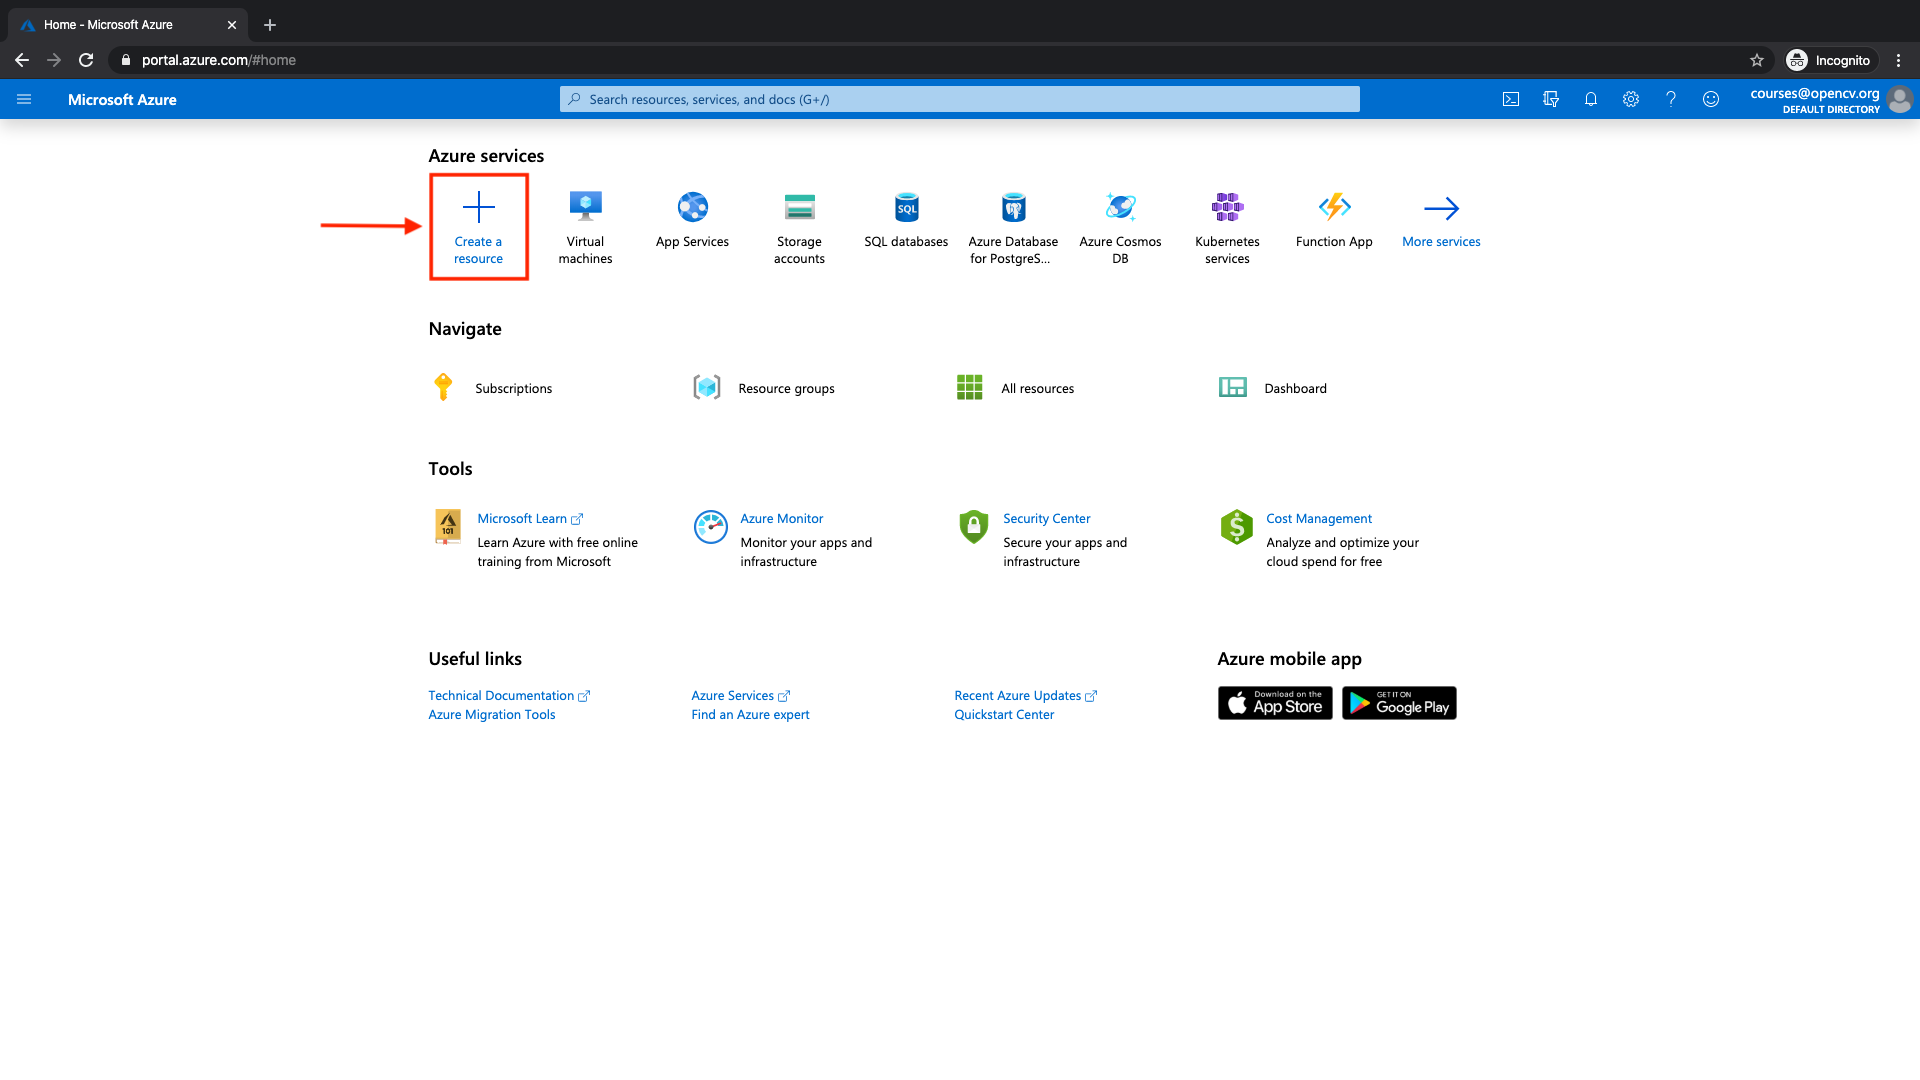
\includegraphics[scale=0.20]{figures/vm1}
%\caption{\small \sl . \cite{Mallick m.fl. 2020} \label{fig:azure}}
\end{center}
\end{figure}

2. Search for Data Science Virtual Machine and choose the one with 18.04 as shown.

\begin{figure}[H]
\begin{center} 
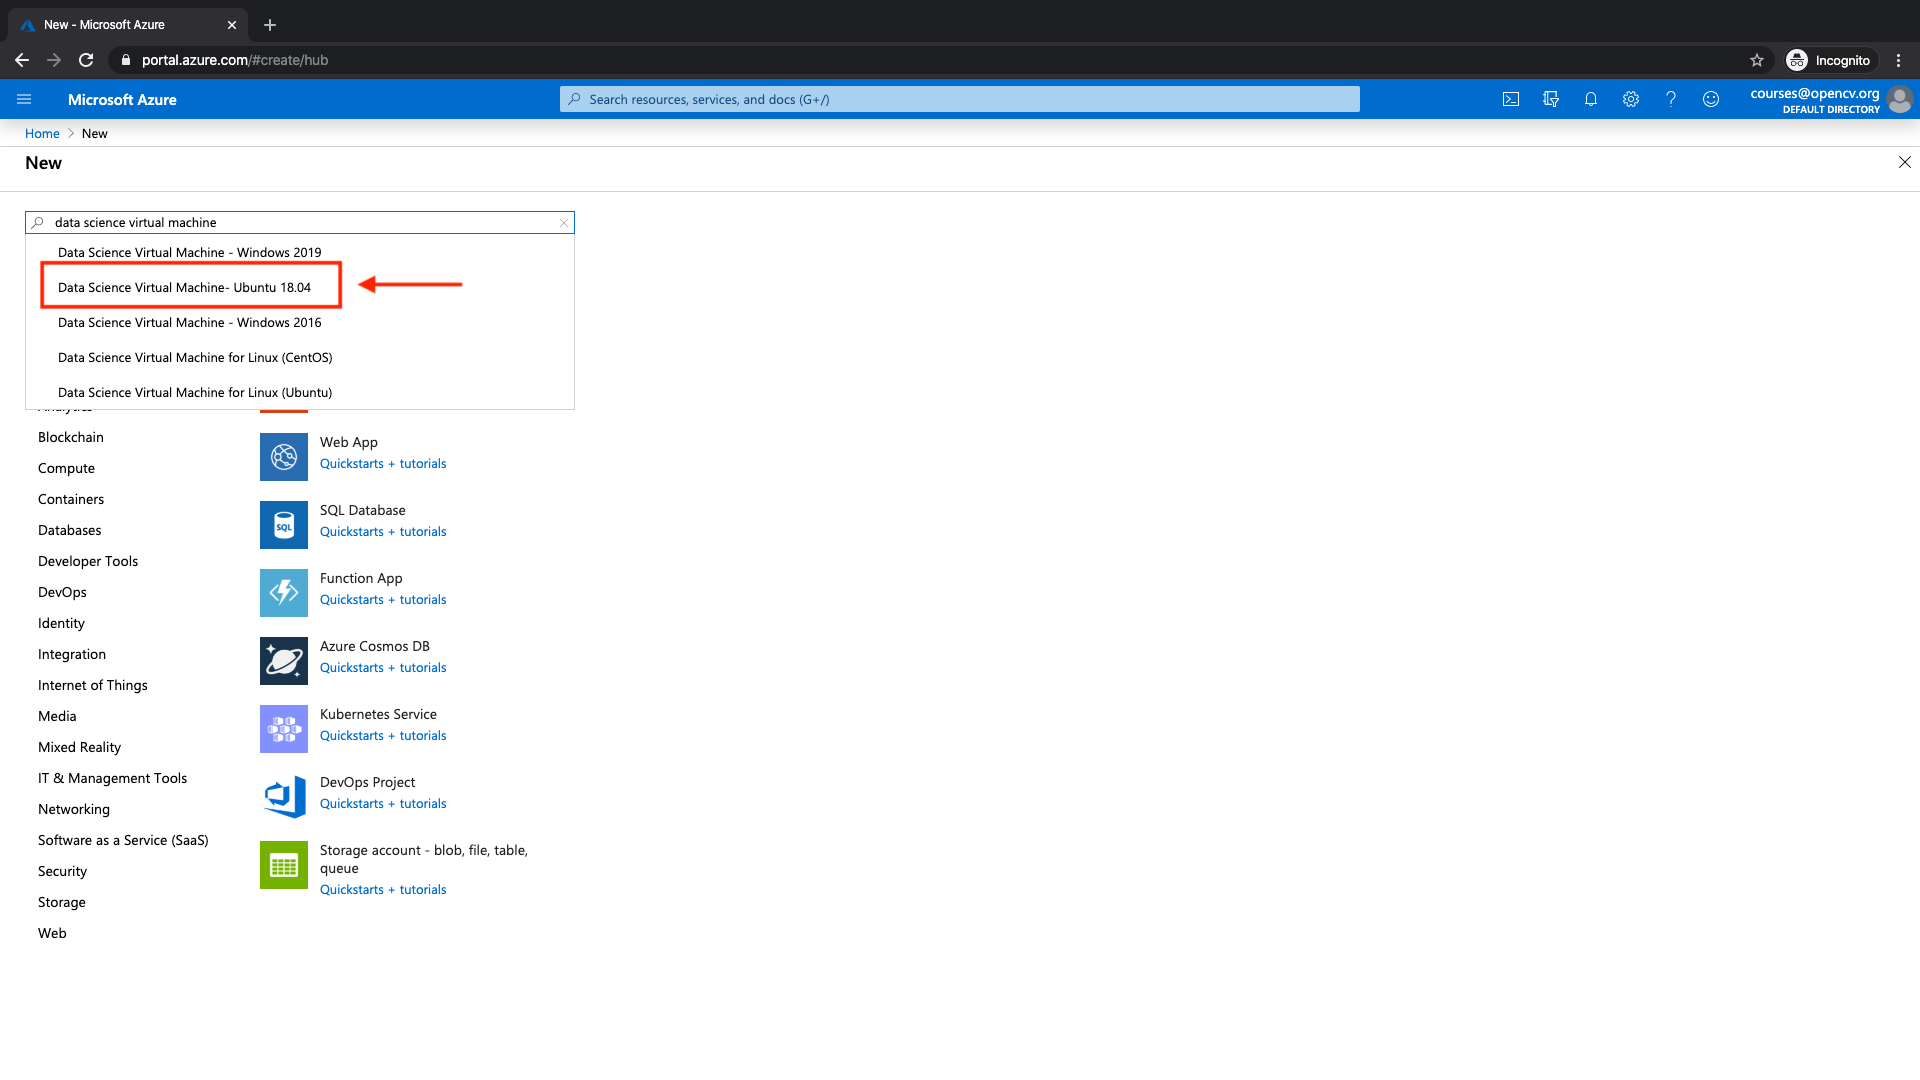
\includegraphics[scale=0.20]{figures/vm2}
%\caption{\small \sl . \cite{Mallick m.fl. 2020} \label{fig:azure}}
\end{center}
\end{figure}

3. Once you select the VM image, you can click on Create.

\begin{figure}[H]
\begin{center} 
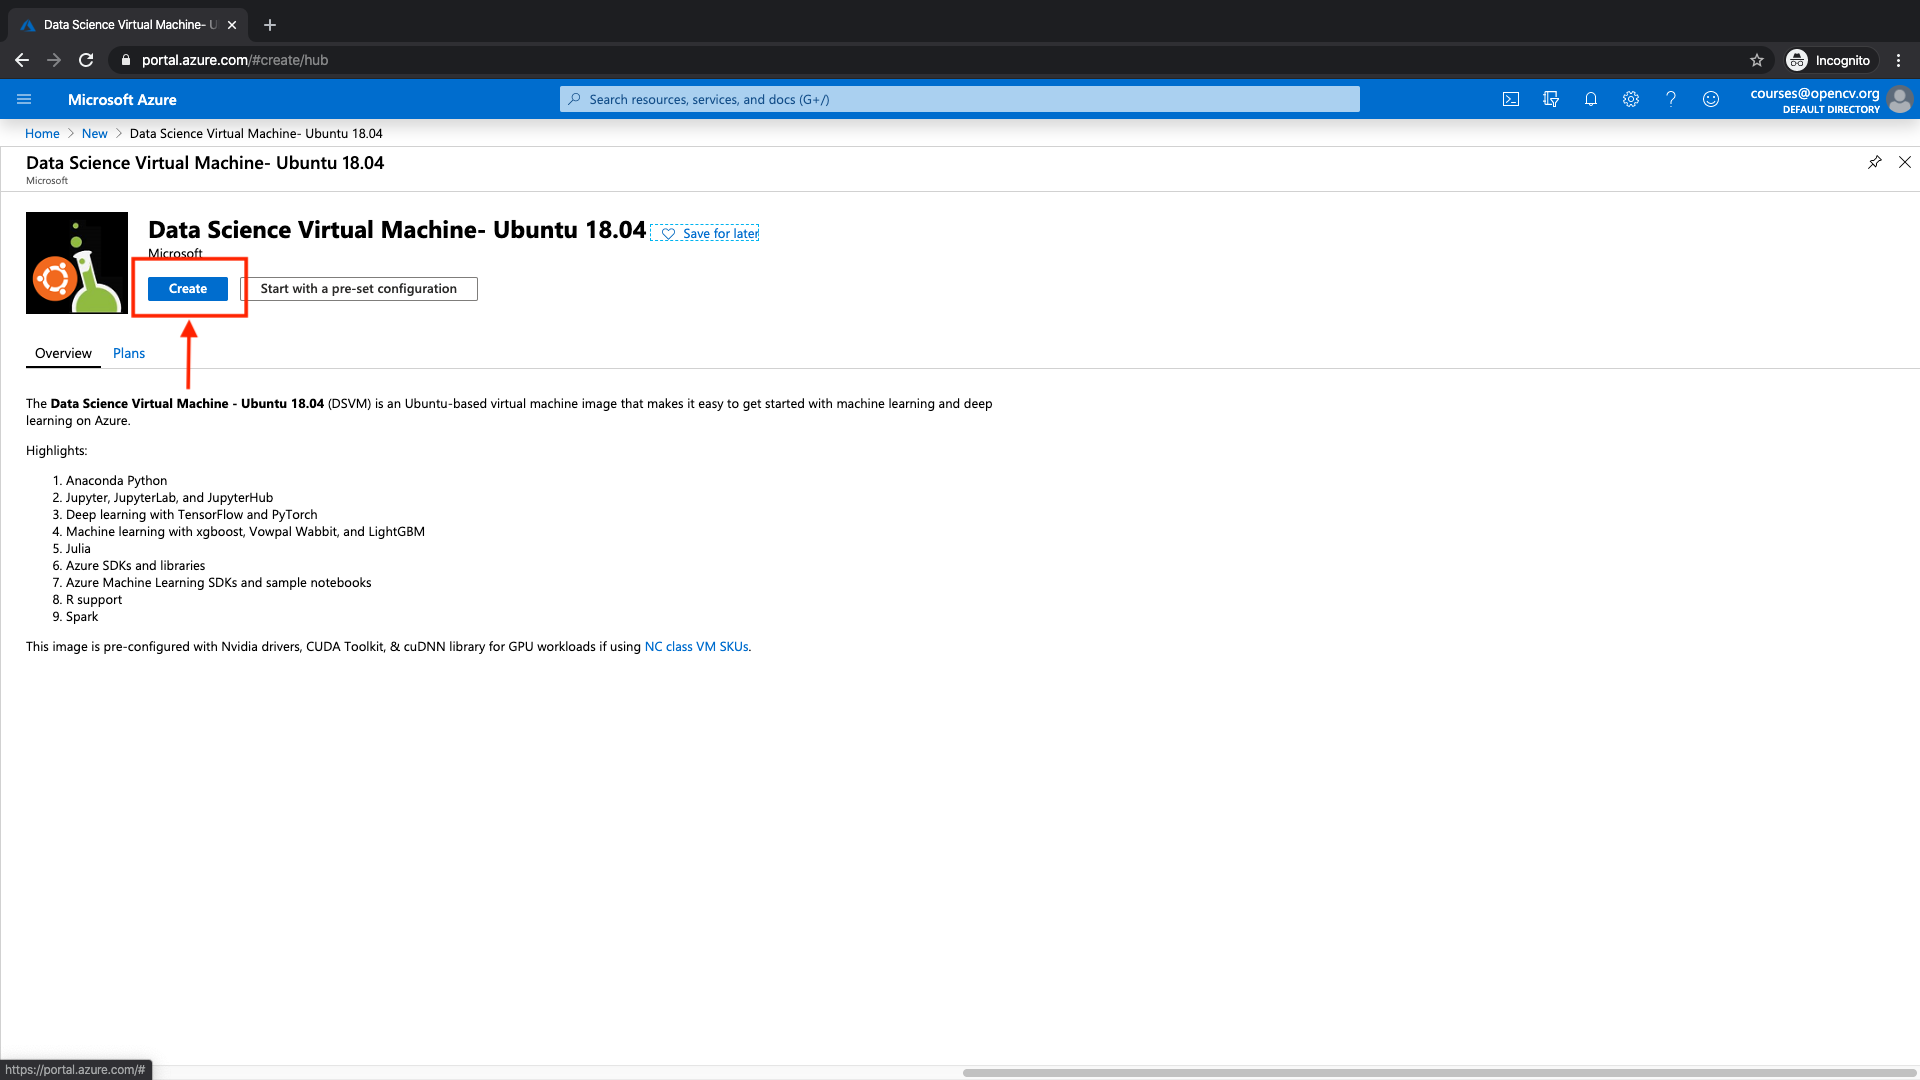
\includegraphics[scale=0.20]{figures/vm3}
%\caption{\small \sl . \cite{Mallick m.fl. 2020} \label{fig:azure}}
\end{center}
\end{figure}

4. Create New Resource Group as shown

\begin{figure}[H]
\begin{center} 
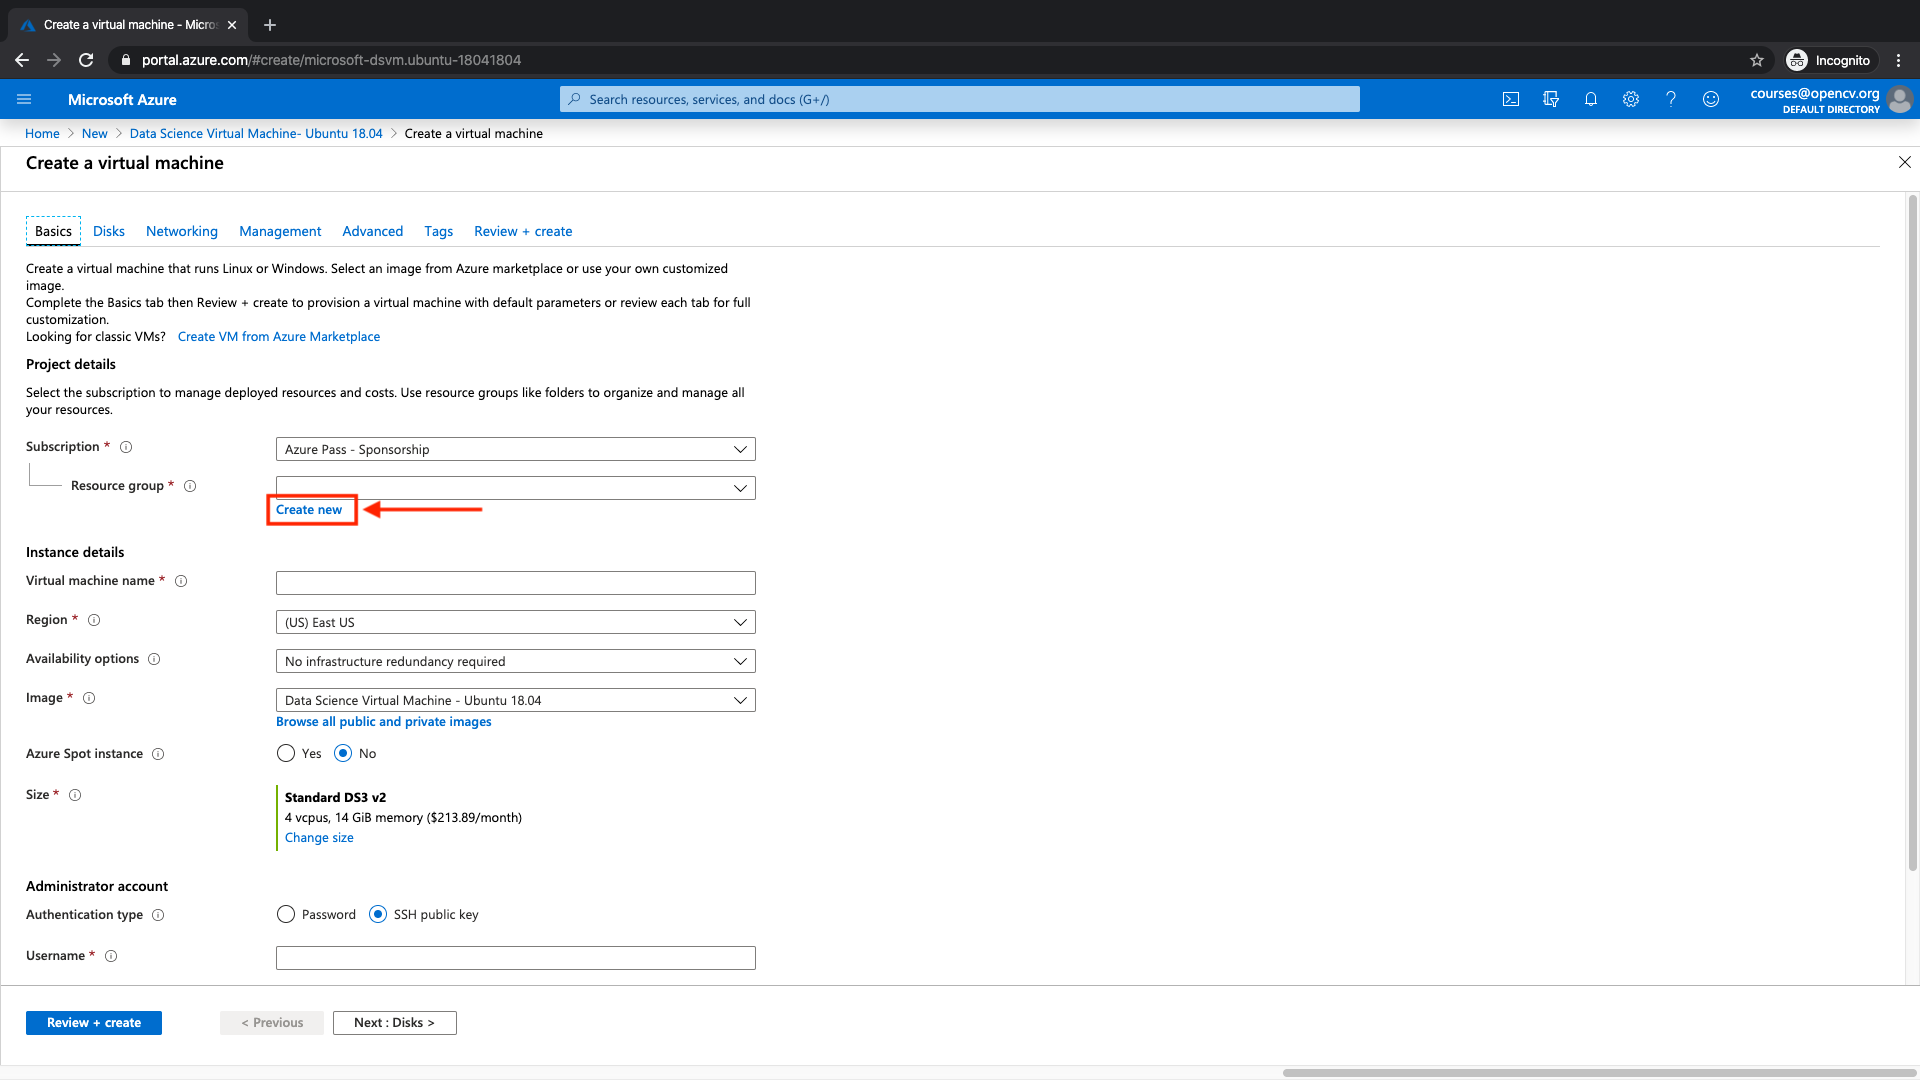
\includegraphics[scale=0.20]{figures/vm4}
%\caption{\small \sl . \cite{Mallick m.fl. 2020} \label{fig:azure}}
\end{center}
\end{figure}

5. You can provide any name of your choice. This can be reused when you create more VMs later.

\begin{figure}[H]
\begin{center} 
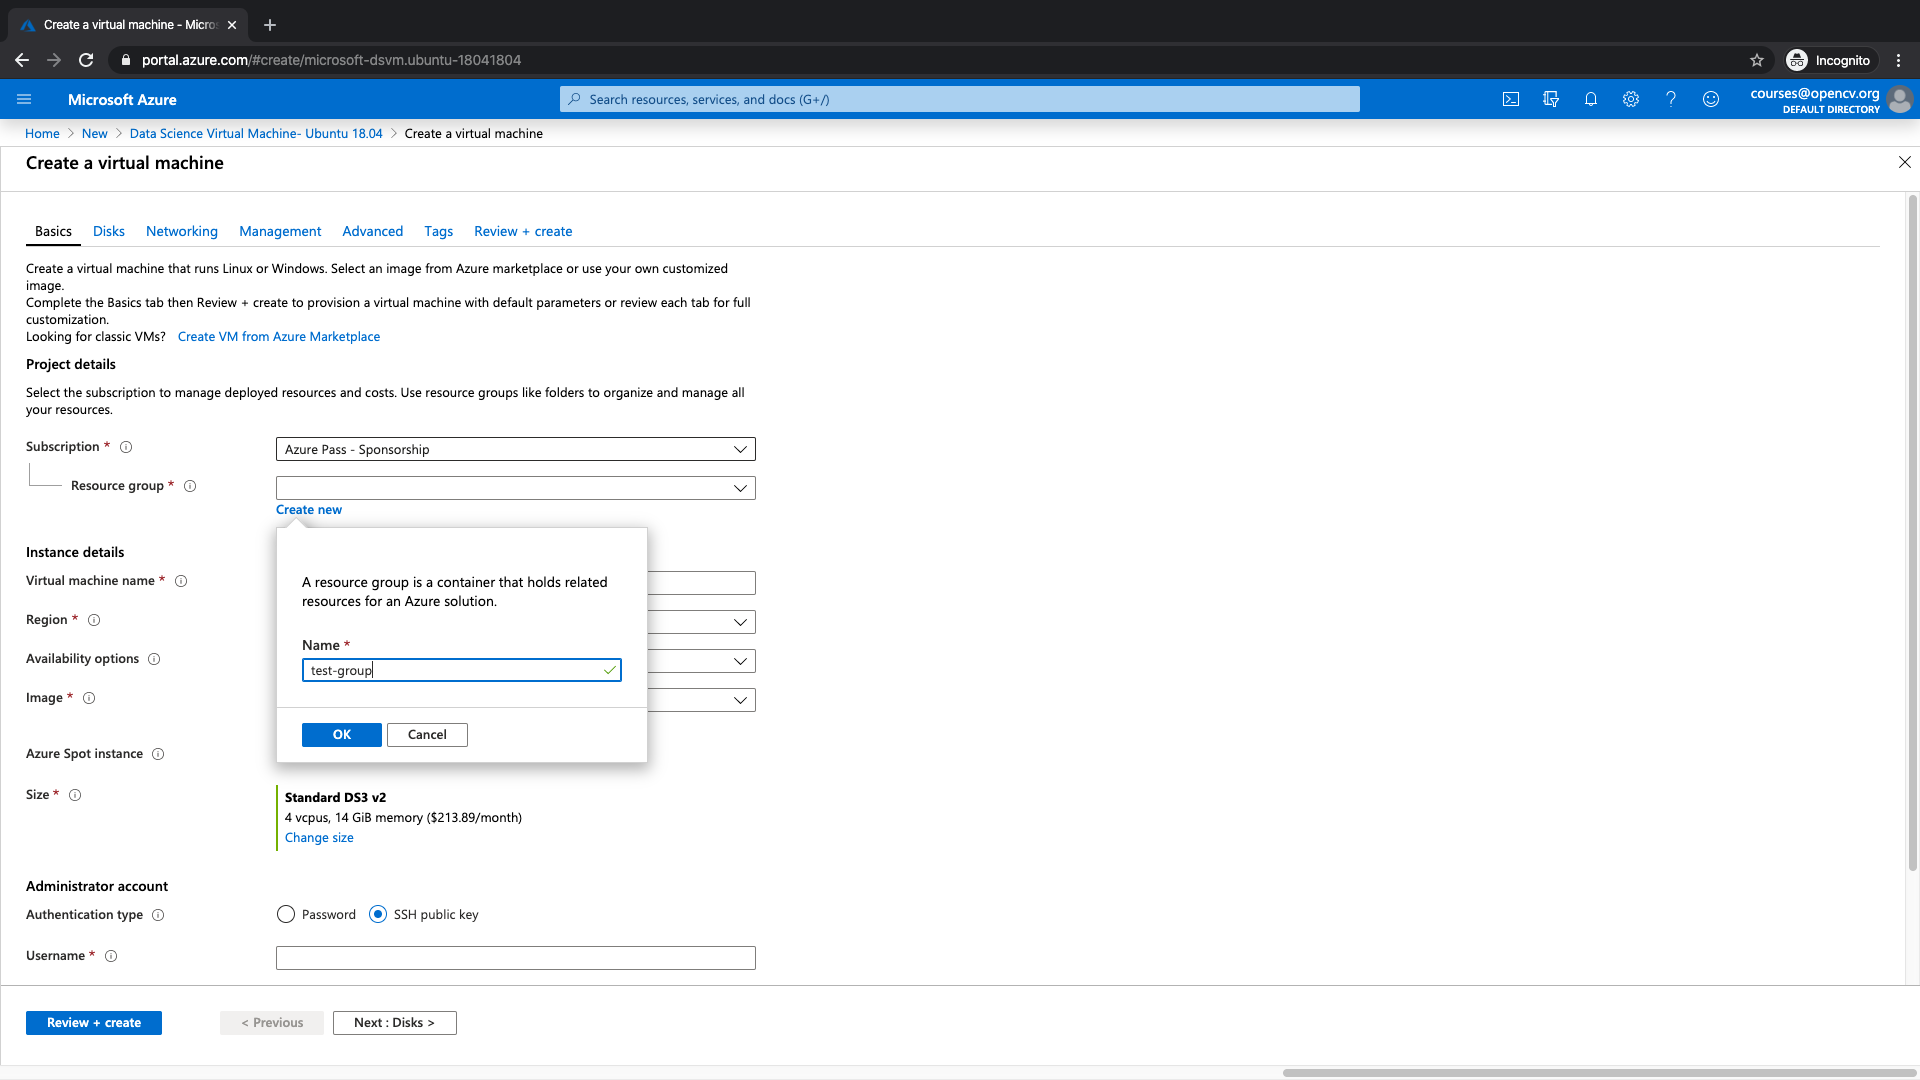
\includegraphics[scale=0.20]{figures/vm5}
%\caption{\small \sl . \cite{Mallick m.fl. 2020} \label{fig:azure}}
\end{center}
\end{figure}

6. Provide a name for your machine

\begin{figure}[H]
\begin{center} 
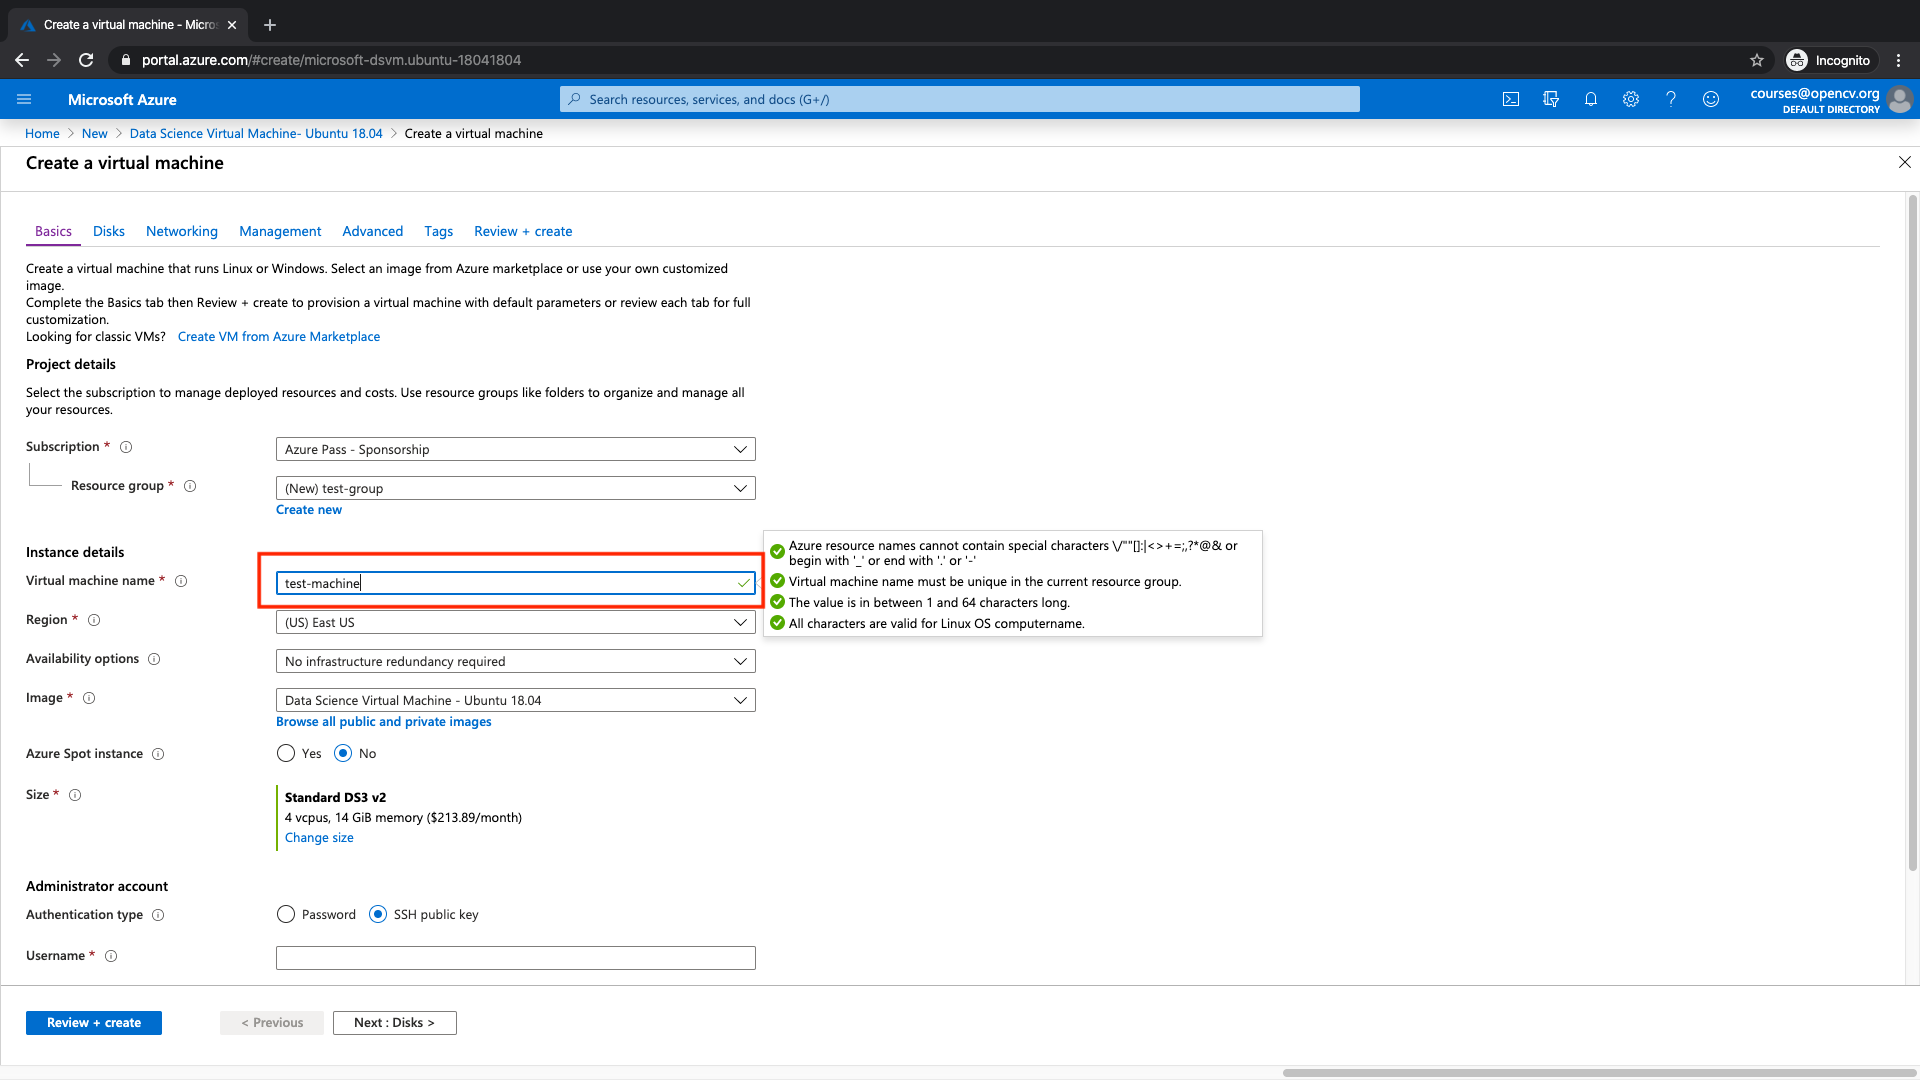
\includegraphics[scale=0.20]{figures/vm6}
%\caption{\small \sl . \cite{Mallick m.fl. 2020} \label{fig:azure}}
\end{center}
\end{figure}

7. Select the Region.
A few important points to note about regions:

1. All types of instances are not available in all regions. Generally, regions in the US and Europe have instances of all types. So, it is advisable to select US/Europe regions even if you are not from these regions.

2. An example where you may want to switch regions is that you may not find the required instance in that particular region at any given time. For example, I was able to select NC6\_Promo instance from US East. But when I checked later, there were no available instances of type NC6\_Promo in US East, so I had to choose US West 2.

3. Pricing varies among different regions. I have generally found US East, US West 2, and US North Central to be cheaper.

Here, we have selected US East region.

\begin{figure}[H]
\begin{center} 
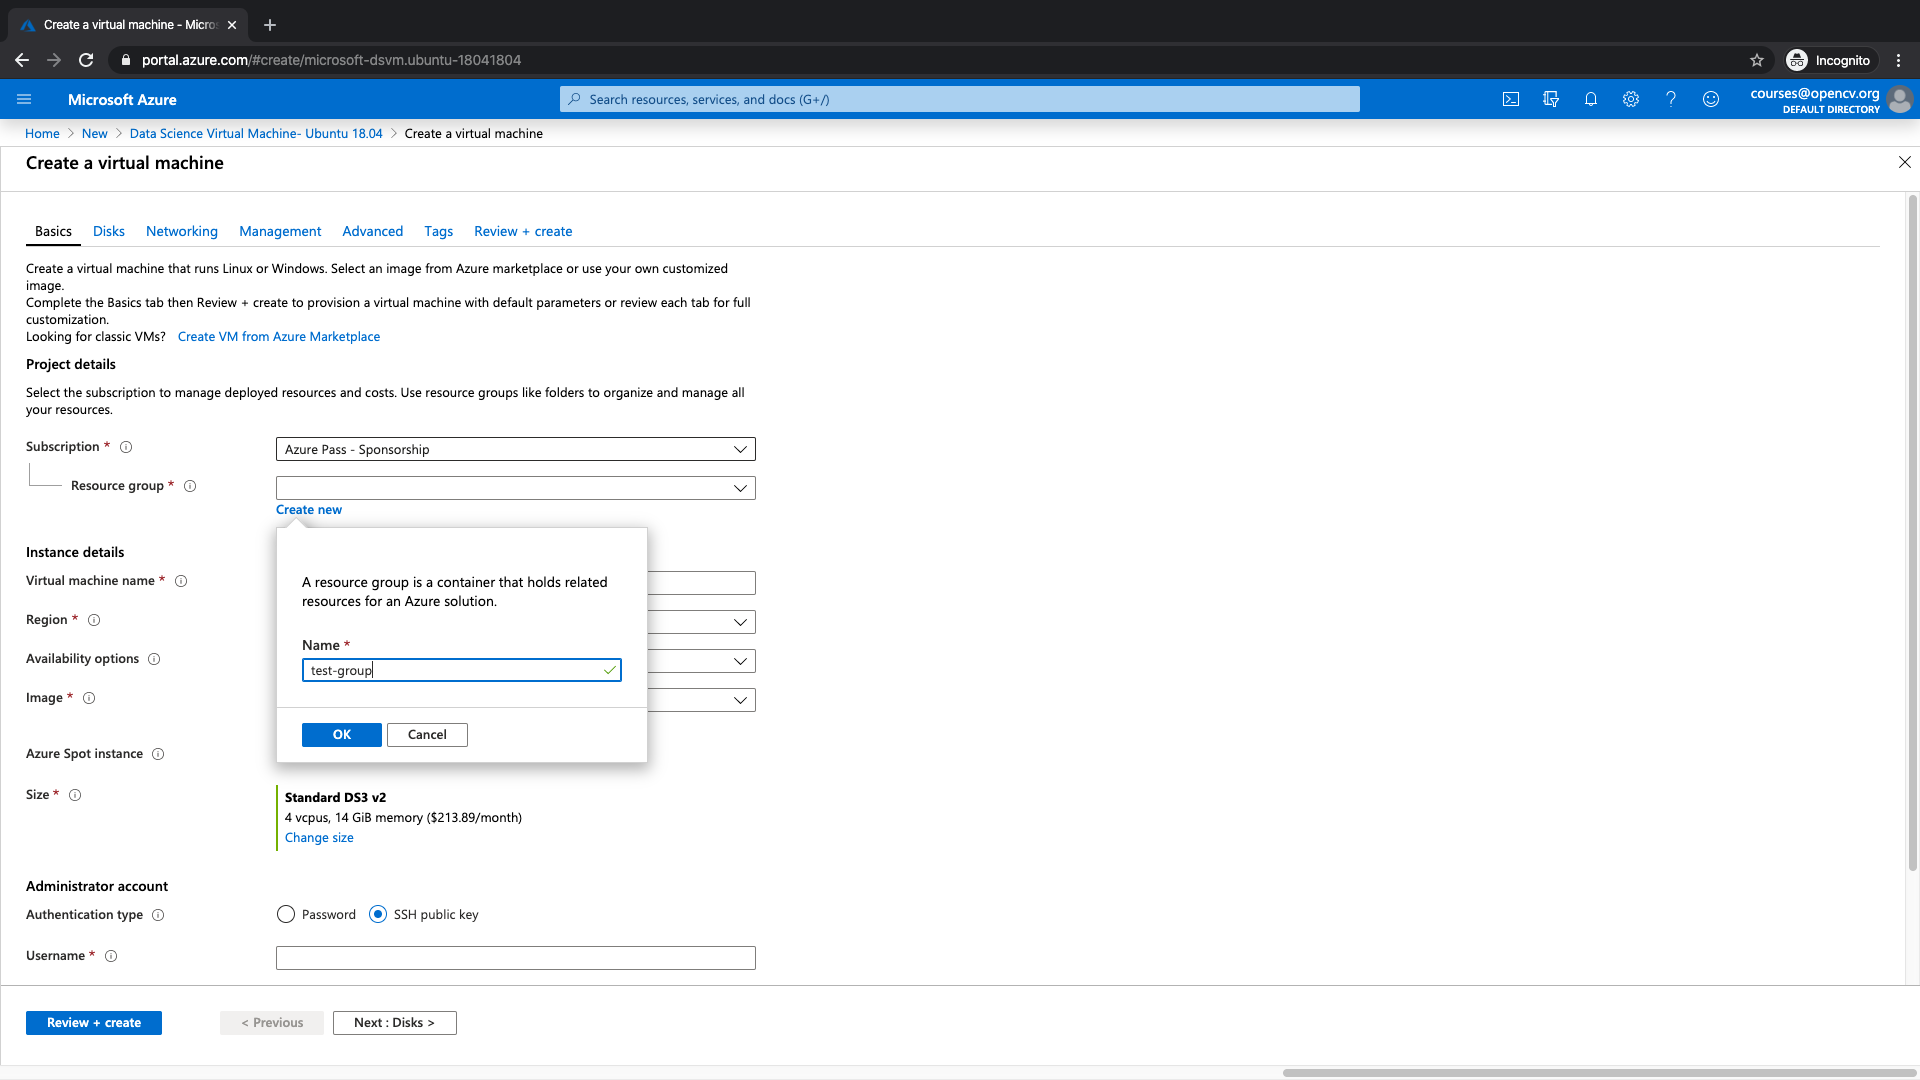
\includegraphics[scale=0.20]{figures/vm5}
%\caption{\small \sl . \cite{Mallick m.fl. 2020} \label{fig:azure}}
\end{center}
\end{figure}

8. Change the type of Instance
We want to use a GPU instance. Low-cost GPU instances are named NCx\_Promo where x can be 6, 12 etc. We will select NC6\_Promo. 

\begin{figure}[H]
\begin{center} 
\includegraphics[scale=0.20]{figures/vm6}
%\caption{\small \sl . \cite{Mallick m.fl. 2020} \label{fig:azure}}
\end{center}
\end{figure}

Note that if you do not find NC6\_Promo in the selected region then you should try changing the region until you find the desired instance type.

Let us change the instance type.

9. Clear default filters

\begin{figure}[H]
\begin{center} 
\includegraphics[scale=0.20]{figures/vm7}
%\caption{\small \sl . \cite{Mallick m.fl. 2020} \label{fig:azure}}
\end{center}
\end{figure}

10. Add Filter for GPU instances
We will apply the filter of GPU family of instances as shown in the 3 screenshots below.

\begin{figure}[H]
\begin{center} 
\includegraphics[scale=0.20]{figures/vm8}
%\caption{\small \sl . \cite{Mallick m.fl. 2020} \label{fig:azure}}
\end{center}
\end{figure}

\begin{figure}[H]
\begin{center} 
\includegraphics[scale=0.20]{figures/vm9}
%\caption{\small \sl . \cite{Mallick m.fl. 2020} \label{fig:azure}}
\end{center}
\end{figure}

\begin{figure}[H]
\begin{center} 
\includegraphics[scale=0.20]{figures/vm10}
%\caption{\small \sl . \cite{Mallick m.fl. 2020} \label{fig:azure}}
\end{center}
\end{figure}

11. Select the NC6\_Promo instance
You can see the information about the instance, for example it is from the GPU family and has 6 vCPUs, 56GB of RAM, storage of 380GB and the price is 289 dollar.

\begin{figure}[H]
\begin{center} 
\includegraphics[scale=0.20]{figures/vm11}
%\caption{\small \sl . \cite{Mallick m.fl. 2020} \label{fig:azure}}
\end{center}
\end{figure}

\begin{figure}[H]
\begin{center} 
\includegraphics[scale=0.20]{figures/vm12}
%\caption{\small \sl . \cite{Mallick m.fl. 2020} \label{fig:azure}}
\end{center}
\end{figure}

12. Check the updated instance
Check if the instance has changed according to your selection.

\begin{figure}[H]
\begin{center} 
\includegraphics[scale=0.20]{figures/vm13}
%\caption{\small \sl . \cite{Mallick m.fl. 2020} \label{fig:azure}}
\end{center}
\end{figure}

13. Set up username and Password
For logging into the system, you can use ssh. But for using jupyter Notebooks directly, you need to set a username and password. These credentials can be used while logging in to the system as well as accessing jupyter notebooks as we will see later.

\begin{figure}[H]
\begin{center} 
\includegraphics[scale=0.20]{figures/vm14}
%\caption{\small \sl . \cite{Mallick m.fl. 2020} \label{fig:azure}}
\end{center}
\end{figure}

14. Select Disks
We do not have to change anything here. If you want to add separate disks, then you have to edit this step accordingly.

\begin{figure}[H]
\begin{center} 
\includegraphics[scale=0.20]{figures/vm15}
%\caption{\small \sl . \cite{Mallick m.fl. 2020} \label{fig:azure}}
\end{center}
\end{figure}

15. Set up Networking
We just keep the defaults.

\begin{figure}[H]
\begin{center} 
\includegraphics[scale=0.20]{figures/vm18}
%\caption{\small \sl . \cite{Mallick m.fl. 2020} \label{fig:azure}}
\end{center}
\end{figure}

16. Configure Management options
You need to specify management options here. Create a new storage account and click next as shown below.

\begin{figure}[H]
\begin{center} 
\includegraphics[scale=0.20]{figures/vm19}
%\caption{\small \sl . \cite{Mallick m.fl. 2020} \label{fig:azure}}
\end{center}
\end{figure}

\begin{figure}[H]
\begin{center} 
\includegraphics[scale=0.20]{figures/vm20}
%\caption{\small \sl . \cite{Mallick m.fl. 2020} \label{fig:azure}}
\end{center}
\end{figure}

17. Advanced options
We will keep the default options.

\begin{figure}[H]
\begin{center} 
\includegraphics[scale=0.20]{figures/vm21}
%\caption{\small \sl . \cite{Mallick m.fl. 2020} \label{fig:azure}}
\end{center}
\end{figure}

18. Add tags
You can add tags to your instances. It is a good practice since you may forget the purpose of each instance when you are dealing with multiple instances. We will add a Name tag so that we know this instance by a name!

\begin{figure}[H]
\begin{center} 
\includegraphics[scale=0.20]{figures/vm22}
%\caption{\small \sl . \cite{Mallick m.fl. 2020} \label{fig:azure}}
\end{center}
\end{figure}

19. Finish Configuration
We are done with the configuration steps and now we can create the instance. Click on Create

\begin{figure}[H]
\begin{center} 
\includegraphics[scale=0.20]{figures/vm23}
%\caption{\small \sl . \cite{Mallick m.fl. 2020} \label{fig:azure}}
\end{center}
\end{figure}

This might take some time. . . ( 5 to 10 minutes )

\begin{figure}[H]
\begin{center} 
\includegraphics[scale=0.20]{figures/vm24}
%\caption{\small \sl . \cite{Mallick m.fl. 2020} \label{fig:azure}}
\end{center}
\end{figure}

20. Check your instance
Once the deployment is done,  you can check out your brand new instance. Click on Go to Resource. ( You can also click on the Home button on top left ).

\begin{figure}[H]
\begin{center} 
\includegraphics[scale=0.20]{figures/vm25}
%\caption{\small \sl . \cite{Mallick m.fl. 2020} \label{fig:azure}}
\end{center}
\end{figure}

\begin{figure}[H]
\begin{center} 
\includegraphics[scale=0.20]{figures/vm26}
%\caption{\small \sl . \cite{Mallick m.fl. 2020} \label{fig:azure}}
\end{center}
\end{figure}

You can see that your instance is created and it has been assigned a public IP address which you can use to login.

%\clearpage
\pagenumbering{arabic}
\setcounter{page}{1}

\pagestyle{fancy}
%\fancyhf{}
\rhead{Vedlegg C side \thepage}
%\lhead{Guides and tutorials}

\section{SSH guide}
\label{appendix:ssh}

\end{document}
